% % % % % % % %  MDT UFSM 2021  % % % % % % % % 
%% Arquivo base para o documento - ver. 1.0 %%
% % % % % % % % % % % % % % % % % % % % % % % % 


% % % OPCOES DE COMPILACAO
% % % PAGINACAO
% % % PAGINACAO SIMPLES (FRENTE): PARA TRABALHOS COM MENOS DE 100 PAGINAS
\documentclass[oneside,openright,12pt]{ufsm_2021} %%%%% OPCAO PADRAO -> PAGINACAO SIMPLES. PARA TRABALHOS COM MAIS DE 100 PAGINAS COMENTE ESTA LINHA E DESCOMENTE A LINHA 
% % % % % % % % % % % % % % % % % % % % % % % % % % % % % % % % % % % % % % %
% PAGINACAO DUPLA (FRENTE E VERSO): PARA TRABALHOS COM MAIS DE 100 PAGINAS
% \documentclass[twoside,openright,12pt]{ufsm_2021}  %%%% PARA TRABALHOS COM MAIS DE 100 PAGINAS DESCOMENTE AQUI
% % % % % % % % % % % % % % % % % % % % % % % % % % % % % % % % % % % % %




% % % %  CODIFICACAO DO TEXTO 
% % % %  POR PADRAO USA-SE UTF8. PARA APLICAR A CODIFICACAO OESTE EUROPEU (ISO 8859-1) DESCOMENTE A LINHA ABAIXO. ELA ATIVA A OPCAO "latin1" DO PACOTE "inputenc"
% \oesteeuropeu
% % % % % % % % % % % 



% % % % % % % % PACOTES PESSOAIS % % % % % % % %  
\usepackage{lipsum}
\usepackage{quoting}
\usepackage{gensymb}


% % % % % % % % DEFINICOES PESSOAIS % % % % % % % %







% % % % % % % % % % % % % % % % % % % % % % % % % % % % % % % % % % % % % % % % % % % 




% % % % % % % % % % % % % % % % % % % % % % % % % % % % % % % % % 
% % % % % % % % % % % % DADOS DO TRABALHO % % % % % % % % % % % % 
% % % % % % % % % % % % % % % % % % % % % % % % % % % % % % % % % 

% % % % % % % % % % INFORMACOES INSTITUCIONAIS % % % % % % % % % % 


% % CENTRO DE ENSINO DA UFSM
\centroensino{Centro de Tecnologia}  %%% NOME POR EXTENSO
\centroensinosigla{CT}  %%% SIGLA

% % CURSO DA UFSM
\nivelensino{Bacharelado}  %%%%%%% NIVEL DE ENSINO 
\curso{Engenharia Aeroespacial}   %%%%% NOME POR EXTENSO
\ppg{EA}   %%%%%% SIGLA
\statuscurso{Curso}  %%%% STATUS= {Programa} ou {Curso}
% \EAD  %%%% para cursos EAD
% % % %  LOCAL DO CAMPUS OU POLO
\cidade{Santa Maria}
\estado{RS}


% % % % % % % % % % INFORMACOES DO AUTOR % % % % % % % % % % 
\author{Augusto Pozzebon, Lucas Lira Sassett, Luiz Henrique Schaffazick, Mathias Diettrich}   %%%%% AUTOR DO TRABALHO
\sexo{M} %%%% SEXO DO AUTOR -> M=masculino   F=feminino (IMPORTANTE PARA AJUSTAR PAGINAS PRE-TEXTUAIS)
\grauensino{Bacharel}    %%%%%%%% GRAU DE ENSINO A SER CONCLUIDO
\grauobtido{Bacharelado}    %%%%% TITULO OBTIDO
%\email{lalala@uhul.com}   %%%% E-MAIL PARA CATALOGRAFICA (COPYRIGHT) - OBRIGATORIO
%\endereco{Rua das abobrinhas, n. 666} %%%% TELEFONE PARA CATALOGRAFICA (COPYRIGHT) (CAMPO OPICIONAL -- CASO NAO POSSUA OU NAO QUEIRA DIVULGAR COMENTE A LINHA)
%\fone{11 2222 3333}   %%%% TELEFONE PARA CATALOGRAFICA (COPYRIGHT) FORMATO {11 2222 3333} (CAMPO OPICIONAL -- CASO NAO POSSUA OU NAO QUEIRA DIVULGAR COMENTE A LINHA)
%\fax{11 2222 3333}   %%%% FAX PARA CATALOGRAFICA (COPYRIGHT) FORMATO {11 2222 3333} (CAMPO OPICIONAL -- CASO NAO POSSUA OU NAO QUEIRA DIVULGAR COMENTE A LINHA)


% % % % % % % % % % INFORMACOES DA BANCA % % % % % % % % % % 
% OBSERVACOES: O CAMPO ORIENTADOR EH OBRIGATORIO E NAO DEVE SER COMENTADO
% % % % % %    OS DEMAIS MEMBROS DA BANCA (COOREIENTADOR E DEMAIS PROFESSORES) QUANDO COMENTADOS NAO APARECEM NA FOLHA DE APROVACAO (O LAYOUT DA FOLHA DE APROVACAO ESTA PREPARADO PARA O ORIENTADOR E ATE MAIS 4 MEMBROS NA BANCA
\orientador{André Luis da Silva}{Dr}{AAAA}{M}{P}  %%%INFORMACOES SOBRE ORIENTADOR: OS CAMPOS SAO:{NOME}{SIGLA DA TITULACAO}{SIGLA DA INSTITUICAO DE ORIGEM}{SEXO} M=masculino   F=feminino {PARTE DA BANCA?} P=presidente  M=Membro  N=Nao faz parte
%\coorientador{Maria da Costa}{Dra}{AAAA}{F}{M} %%%INFORMACOES SOBRE CO-ORIENTADOR: OS CAMPOS SAO:{NOME}{SIGLA DA TITULACAO}{SIGLA DA INSTITUICAO DE ORIGEM}{SEXO} M=masculino   F=feminino {PARTE DA BANCA?} P=presidente  M=Membro  N=Nao faz parte
%\bancaum{Banca Um}{Dr}{AAAA}{F}{M}  %%%INFORMACOES SOBRE PRIMEIRO NOME DA BANCA: OS CAMPOS SAO:{NOME}{SIGLA DA TITULACAO}{SIGLA DA INSTITUICAO DE ORIGEM}{SEXO} M=masculino   F=feminino {PARTE DA BANCA?} P=presidente  M=Membro  N=Nao faz parte
%\bancadois{Banca Dois}{Dr}{BBBB}  %%%INFORMACOES SOBRE SEGUNDO NOME DA BANCA: OS CAMPOS SAO:{NOME}{SIGLA DA TITULACAO}{SIGLA DA INSTITUICAO DE ORIGEM}
% \bancatres{Banca Três}{Dra}{CCCC} %%%INFORMACOES SOBRE TERCEIRO NOME DA BANCA: OS CAMPOS SAO:{NOME}{SIGLA DA TITULACAO}{SIGLA DA INSTITUICAO DE ORIGEM}
% \bancaquatro{Banca Quatro}{Dr}{DDDD} %%%INFORMACOES SOBRE QUARTO NOME DA BANCA: OS CAMPOS SAO:{NOME}{SIGLA DA TITULACAO}{SIGLA DA INSTITUICAO DE ORIGEM}
% \bancacinco{Banca Cinco}{Dra}{EEEE} %%%INFORMACOES SOBRE QUARTO NOME DA BANCA: OS CAMPOS SAO:{NOME}{SIGLA DA TITULACAO}{SIGLA DA INSTITUICAO DE ORIGEM}
% \supervisor{Al Paccino}{Dr}{MAFIA}{M}{N} %%%INFORMACOES SOBRE SUPERVISOR (indicado para estagios): OS CAMPOS SAO:{NOME}{SIGLA DA TITULACAO}{SIGLA DA INSTITUICAO DE ORIGEM}{SEXO} M=masculino   F=feminino {PARTE DA BANCA?} P=Presidente  M=Membro  N=Nao faz parte



% % % % % % % % % % REALIZACAO POR VIDEO CONFERENCIA (MEMORANDO 04/2016 BIBLIOTECA CENTRAL UFSM)
%\videoconferencia % % % % QUANDO O ACADEMICO DEFENDE POR VIDEO CONFERENCIA (PERMITIDO PELO ARTIGO 82 DO REGIMENTO GERAL DA PRPGP/UFSM). PARA DEFESAS NAS QUAIS O ACADEMICO ESTA PRESENTE COMENTE ESTA LINHA
% % % % QUANDO UM DOS MEMBROS DA BANCA PARTICIPA POR VIDEO CONFERENCIA INDICAR O MEMBRO DE ACORDO COM A LISTA ABAIXO. CASO CONTRARIO MANTER A PALAVRA "NAO". SAO PERMITIDOS, PELO REGIMENTO PRGPGP (ARTIGO 83) ATE 2 MEMBROS 
%\videoconferenciabancap{NAO}  %%%% PRIMEIRO MEMBRO
%\videoconferenciabancas{NAO}  %%%%% SEGUNDO MEMBRO
% % O > ORIENTADOR
% % CO > COORIENTADOR% % % % QUANDO UM DOS MEMBROS DA BANCA PARTICIPA POR VIDEO CONFERENCIA INDICAR O MEMBRO DE ACORDO COM A LISTA ABAIXO. CASO CONTRARIO MANTER A PALAVRA "NAO". SAO PERMITIDOS, PELO REGIMENTO PRGPGP ATE 2 MEMBROS.
% % 1 > BANCA UM
% % 2 > BANCA DOIS
% % 3 > BANCA TRÊS
% % 4 > BANCA QUATRO
% % 5 > BANCA CINCO
% % S > SUPERVISOR
% % % % % % % % % % % % % % % % % % % % % % % % % % % % % % % % % % % % 



% % % % % % % % % % INFORMACOES SOBRE O TRABALHO % % % % % % % % % %
% % % %  TITULO E SUBTITULO DO TRABALHO: ELES NÃO DEVEM ULTRAPASSAR, JUNTOS, 3 LINHAS NA COMPILAÇÃO DA CAPA. 
% SE O TRABALHO POSSUI SUBTITULO, ADICIONE ':' DENTRO DAS CHAVES ABAIXO 
\titulo{Trabalho 1:} %% NAO EH NECESSARIO CAPITALIZAR
% % % %  TITULO DO TRABALHO EM INGLES
% SE O TRABALHO POSSUI SUBTÍTULO, ADICIONE ':' DENTRO DAS CHAVES ABAIXO 
%\englishtitle{Título do trabalho em inglês:}  %% NAO EH NECESSARIO CAPITALIZAR


% % % % O SUBTÍTULO É OPCIONAL, SE NÃO FOR USADO AS LINHAS ABAIXO DEVEM SER COMENTADAS

% SE O TRABALHO POSSUI SUBTÍTULO, ADICIONE ':' DENTRO DAS CHAVES ABAIXO 
\subtitulo{Mecânica de Voo Espacial} %% NAO EH NECESSARIO CAPITALIZAR
% % % %  SUB TITULO DO TRABALHO EM INGLES
%\subenglishtitle{Subtítulo do trabalho em inglês}  %% NAO EH NECESSARIO CAPITALIZAR

% % % AREA DE CONCENTRACAO DO TRABALHO (CNPQ)
%\areaconcentracao{Área de concentração do CNPq}
% % % TIPO DE TRABALHO - MANTER APENAS UMA LINHA DESCOMENTADA
%\tese  %% Tese de <nivel de ensino>
% \qualificacao %% Exame de Qualificação de <nivel de ensino>
% \dissertacao %% Dissertacao de <nivel de ensino>
% \monografia %% Monografia
% \monografiag  %% Monografia (nao exibe area de concentracao)
% \tf  %% Trabalho Final de <nivel de ensino>
% \tfg  %% Trabalho Final de Graduacao (nao exibe area de concentracao)
% \tcc  %% Trabalho de Conclusao de Curso
% \tccg  %% Trabalho de Conclusao de Curso (nao exibe area de concentracao)
% \relatorio  %% Relatório de Estágio (nao exibe area de concentracao)
%  \generico   %%% Alternativa para aqueles cursos que nao recebem o titulo de bacharel ou licenciado. Ex: engenharia, arquitetura, etc... Os campos abaixo tambem devem ser preenchidos
     \tipogenerico{Trabalho Avaliativo}
%     \tipogenericoen{Tipo de trabalho em inglês}
%     \concordagenerico{o}
%     \graugenerico{Engenheiro Eletricista}
% % % DATA DA DEFESA 
\data{14}{05}{2023} %% FORMATO {DD}{MM}{AAAA}



% % % % %  ALGUMAS ENTRADAS PRE-TEXTUAIS
% % % % CASO NAO QUEIRA UTILIZA-LAS COMENTE A LINHA DE COMANDO
% % % EPIGRAFE
%\epigrafe{Winter is coming!}{Família Stark} %ESTRUTURA DE CAMPOS -> {Texto}{Autor}
% % % DEDICATORIA
%\dedicatoria{Aos que virão depois de nós}
% % % %  AGRADECIMENTOS
%\agradecimentos{A mim!}

% % % % %  RESUMO E PALAVRAS CHAVE DO RESUMO - OBRIGATORIO PARA MDT-UFSM
\resumo{
Este trabalho explora o complexo campo da mecânica de voo orbital através de uma abordagem pragmática e computacional, utilizando a linguagem de programação Python. O estudo se concentra na compreensão e resolução de uma variedade de tópicos relevantes, incluindo o cálculo da gravidade de um planeta axissimétrico, a propagação da órbita, a determinação da órbita, as manobras orbitais, as órbitas perturbadas e o problema de três corpos restrito. As aplicações práticas desses conceitos na engenharia aeroespacial são discutidas em detalhes, destacando a importância da mecânica de voo orbital para o progresso da exploração espacial. Os resultados obtidos reafirmam a eficácia da abordagem computacional, com as soluções dos exercícios propostos demonstrando sucesso e precisão.
}
\palavrachave{Mecânica de Voo Orbital. Programação Python. Aplicações práticas.}
% "... deverão constar, no mínimo, três palavras-chave, iniciadas em
% letras maiúsculas, cada termo separado dos demais por ponto, e
% finalizadas também por ponto." MDT 2012

% % % % %  ABSTRACT E PALAVRAS CHAVE DO RESUMO - OBRIGATORIO PARA MDT-UFSM
%\abstract{
%Write your abstract here! As recomendações do resumo também se aplicam ao abstract. \lipsum[0-1]
%}
%\keywords{Keyword 1. Keyword 2. Keyword 3. (...)}


% % %  ATIVACAO DE LISTAS E PAGINAS ESPECIAIS
% % %  PARA QUE APARECAO NAO NO TEXTO DESCOMENTE A LINHA ABAIXO -> POR PADRAO TODAS ESTAO ATIVIDADAS

% % LISTA DE FIGURAS 
% \semfiguras   %%(QUANDO ATIVIDA NAO EXIBE A LISTA)
% % LISTA DE GRAFICOS 
 \semgraficos   %%(QUANDO ATIVIDA NAO EXIBE A LISTA)
% % LISTA DE ILUSTRACOES 
 \semilustracoes  %%(QUANDO ATIVIDA NAO EXIBE A LISTA)
% % LISTA DE TABELAS 
% \semtabelas   %%(QUANDO ATIVIDA NAO EXIBE A LISTA)
% % LISTA DE QUADROS 
\semquadros   %%(QUANDO ATIVIDA NAO EXIBE A LISTA)
% % LISTA DE APENDICES 
 \semapendices  %%(QUANDO ATIVIDA NAO EXIBE A LISTA)
% LISTA DE ANEXOS 
 \semanexos   %%(QUANDO ATIVIDA NAO EXIBE A LISTA)


% % % %  LISTA DE ABREVIATURAS - AMBIENTE TABULAR
%%%%%%%% para não utilizar comente as linhas abaixo.
% \abreviaturamax{SIGLAMAX} %%%% coloque aqui a maior sigla (indentacao)
% \listadeabreviaturas{
% 	SIGLA1 & Nome Completo da Sigla 1 \\
% 	SIGLA2 & Nome Completo da Sigla 2 \\
% 	SIGLAMAX &	Nome Completo da Sigla MAX \\
% }


% % % %  LISTA DE SIGLAS - AMBIENTE TABULAR
%%%%%%%% para não utilizar comente as linhas abaixo.
% \siglamax{SIGLAMAX} %%%% coloque aqui a maior sigla (indentacao)
% \listadesiglas{
% SIGLA1 & Nome Completo da Sigla 1 \\
% SIGLA2 & Nome Completo da Sigla 2 \\
% SIGLAMAX &	Nome Completo da Sigla MAX \\
% }


% % % %  LISTA DE SIMBOLOS
%%%%%%%% OBS: O espaco entre colchetes \item[] e um ambiente matematico
%%%%%%%% para não utilizar comente as linhas abaixo.
% \simbolomax{(Re)2} %%%% coloque aqui o maior simbolo (indentacao)
% \listadesimbolos{
% \item[u_*]	Escala de velocidade de fricção	
% \item[w_*]	Escala de velocidade convectiva
% \item[(Re)^2]	Maior simbolo da lista
% }


% % % FICHA CATALOGRAFICA
% \semcatalografica  %%%%  (QUANDO ATIVIDA NAO EXIBE A FICHA CATALOGRAFICA NECESSITA DO ARQUIVO DA FICHA: ficha_catalografica.pdf
% % % A FICHA CATALOGRAFICA FORNECIDA PELA UFSM EH UM PDF DO TAMANHO A4
% % % EH POSSIVEL GERA-LA NO SITE http://cascavel.ufsm.br/ficha_catalografica/
% % % OS COMANDOS ABAIXO DEFINEM AS MARGENS PARA CORTAR A FICHA FORNECIDA E COLOCA-LA COMO UMA FIGURA NO DOCUMENTO LATEX
% \margemesquerda{1.9}   %%%% CORTE DE MARGEM ESQUERDA EM CM
% \margemdireita{1.5}   %%%% CORTE DE MARGEM DIREITA EM CM
% \margemsuperior{2.75}  %%%% CORTE DE MARGEM SUPERIOR EM CM
% \margeminferior{2.9} %%%% CORTE DE MARGEM INFERIOR EM CM
% % %  DICA: IMPRIMA UMA COPIA DA FICHA CATALOGRAFICA E FACA A MEDIDA DAS MARGENS!





% % FOLHA DE ERRATA (versao rudimentar...pode ser aprimorado)
% % para não utilizar comente as linhas abaixo.
% % deve ser preenchida como um ambiente tabular de quatro colunas:
% % pagina & linha & onde se le & leia-a se \\
% \errata{
% 10   &    10    & errado   & certo \\
% \hline
% 12    &    5     & errado com um texto mais longo & certo agora com um texto mais longo\\
% \hline
% 13   &    3    & $x^2$   & $2x$\\
% }
% % % % % % % % % % % % % % % % % % % % % % % % % % % % % % % % % % % % % % % % % % % % % % 


% % % % % % % % % % % % % % % % % % % % % % % % % % % % % % % % % % % % % % 
% % % % % % % % % % % %  OPCOES DE FORMATACAO % % % % % % % % % % % % % % %
% % % % % % % % % % % % % % % % % % % % % % % % % % % % % % % % % % % % % % 
% % % CAPITULO: por padrao alinhado a esquerda. Para ativar alinhamento centralizado descomente o comando abaixo

% \centralizado  %%%% <<< centraliza todos os capitulos

% % % % % % % % % % % % % % % % % % % % % % % % % % % % % % % % % % % % % %
% % % FONTES: descomente uma das opcoes. caso nenhuma seja ativada a clase usara a fonte padrao do latex

%% helvetica
\usepackage[scaled]{helvet}
\renewcommand*\familydefault{\sfdefault}

%% arial
% \renewcommand{\rmdefault}{phv} % Arial
% \renewcommand{\sfdefault}{phv} % Arial

%%times
% \usepackage{mathptmx}

% % % % % % % % % % % % % % % % % % % % % % % % % % % % % % % % % % % % % % 
% % % % % % % % % % % % % % % % % % % % % % % % % % % % % % % % % % % % % % 
% % % % % % % % % % % % % % % % % % % % % % % % % % % % % % % % % % % % % % 
% % % % % % % % % % % % % % % % % % % % % % % % % % % % % % % % % % % % % % 


% % % % % % % % % % % % % % % % % % % % % % % % % % % % % % % % % % % % % % 
% % % % % % % % % % % % % % % % % % % % % % % % % % % % % % % % % % % % % % 
% % % % % % % % % % % %  INICIO DO DOCUMENTO  % % % % % % % % % % % % % % %
% % % % % % % % % % % % % % % % % % % % % % % % % % % % % % % % % % % % % % 
% % % % % % % % % % % % % % % % % % % % % % % % % % % % % % % % % % % % % %


\begin{document}



% % % % % % % % % % % % % % % % % % % % % % % % % % % % % % % % % % % % % % 
\pretextual  %%%% GERA AS PAGINAS PRE-TEXTUAIS   
% % % % % % % % % % % % % % % % % % % % % % % % % % % % % % % % % % % % % % 

% % % % % % % % % % % % % % % % % % % % % % % % % % % % % % % % % % % % % % 
% % % % % CORPO DO TRABALHO - INCLUA OS SEUS TEXTOS AQUI
% % % % % SUGESTAO -> UTILIZE ARQUIVOS EXTERNOS A PARTIR DO COMANDO \input
% % % % % % % % % % % % % % % % % % % % % % % % % % % % % % % % % % % % % % 
% % % % % % % % % % INICIO DAS PAGINAS TEXTUAIS % % % % % % % % % % % % % % 
% % % % % % % % % % % % % % % % % % % % % % % % % % % % % % % % % % % % % % 

\chapter{Introdução}

\par Este trabalho tem como foco a inserção em órbita geossíncrona de um CubeSat 8U. A primeira etapa desse trabalho é estudar e adaptar um foguete existente para atender aos requisitos de variação de velocidade (∆v), conforme determinado pela equação do foguete. Esta adaptação inclui a verificação da distribuição ideal de massa entre os estágios do foguete, propondo alterações se necessário para otimizar o impulso e, assim, alcançar o ∆v necessário.

O foguete será analisado em termos de voo ascendente, abordando aspectos como inserção em órbita, avaliação da factibilidade em termos de impulso de velocidade, ajuste de distribuição de massa para capacitação de inserção orbital, cálculo de parâmetros inerciais, e avaliação da factibilidade em termos de energia específica, órbita de referência e altitude.

Ademais, será abordado o voo ascendente de foguete em termos de voo balístico e trajetória de rotação gravitacional, bem como o modelo de trajetória plana de voo ascendente. Ajustes de parâmetros para obtenção da órbita desejada, considerando excentricidade e inclinação, serão discutidos.

Além disso, é apresentado o modelo do veículo de inserção orbital e o conceito de rastro planetário, também conhecido como "ground track". Ao final deste trabalho, o objetivo é ter um modelo de foguete capaz de simular a inserção orbital do CubeSat 8U em órbita geossíncrona, desde o lançamento até a aquisição da órbita alvo.
\chapter{Metodologia}

\section{Cálculo da gravidade de planeta axissimétrico}
\subsection{Força gravitacional para massas pontuais}

Para o caso de massas pontuais $m1$ e $m2$, existe uma força gravitacional \textbf{f} que é exercida por ambas as massas e atua sob ambas as massas com mesmo módulo e direção, porém com sentido contrário para cada uma. A equação \ref{eq:grav uni} é a formulação da força \textbf{f} pela lei da gravitação universal de Newton, sendo $G = 6,67259(\pm 0,0003) \times 10^{-11}$ a constante gravitacional e $r$ a distância entre as massas. É possível também descrever a força gravitacional em termos da aceleração da gravidade $g$ da massa $m_{2}$.

\begin{equation}
\textbf{f} = -G\frac{m_{2}m_{1}}{r^{2}} 
\label{eq:grav uni}
\end{equation}

Assim, o módulo da força \textbf{f} é inversamente proporcional ao quadrado da distância $r$, porém esse é o resultado elementar, apenas para massas pontuais, pois no caso de corpos com distribuições não simétricas de massa ocorrem variações na magnitude ou direção da gravidade, influenciando a precisão dos cálculos. 

\subsection{Força gravitacional para corpos contínuos}
Então, para tratar de corpos contínuos com distribuição genérica de massa, é aplicada a equação anterior quando considerada a força exercida sobre uma massa pontual, porém é necessário que o corpo contínuo possa ser aproximado por uma discretização de $N$ massas pontuais, sendo que quanto maior o $N$, mais precisa é a aproximação. Portanto, a força resultante que o corpo contínuo $M$ exerce sobre a massa pontual é a soma vetorial das forças provocadas por todas as massas discretas $m_{i}, i = 1, 2, \dots N$, como mostrado na equação \ref{eq: fresM}. 

\begin{equation}
\textbf{f} = \sum\limits_{i=1}^{\mbox{N}}\textbf{f}_{i} = m \sum\limits_{i=1}^{\mbox{N}}\textbf{g}_{i}
\label{eq: fresM}
\end{equation}

É possível, sem perda de generalidade, transformar esse problema para o campo escalar, isso pois o campo gravitacional é conservativo, levando à definição do potencial gravitacional, mostrado na equação \ref{eq:ptg}, representando o potencial gravitacional da massa $m_{i}$ sobre a massa $m$.

\begin{equation}
\Phi_{i} = \frac{Gm_{i}}{r_{mi}}
\label{eq:ptg}
\end{equation}

A partir do gradiente do potencial gravitacional é possível definir a aceleração da gravidade provocada pelo corpo $m_{i}$. Portanto, a aceleração da gravidade \textbf{g} resultante sobre o corpo de massa $m$ é dada pela equação \ref{eq: 6}.

\begin{equation}
\textbf{g} = \sum\limits_{i=1}^{\mbox{N}}\textbf{g}_{i} = \sum\limits_{i=1}^{\mbox{N}}\frac{\partial \Phi_{i}}{\partial \textbf{r}_{mi}}
\label{eq: 6}
\end{equation}

É interessante trabalhar com somas discretas (\ref{eq: 6}) para poucos termos ou sistemas realmente discretos, porém, nesse caso, a discretização é de um corpo contínuo, então pode-se tomar o limite de $N \rightarrow \infty$, ou seja, as massas pontuais $m_{i}$ em elementos infinitesimais de massa $dm$, assim, a soma discreta \ref{eq: 6} converge para uma integral de volume sobre toda a matéria do corpo $M$.

Para desenvolver matematicamente, é necessário aprofundar a modelagem do problema, o que pode ser feito estabelecendo uma geometria de referência, mostrada na figura \ref{fig:geometriaref}. É tido um sistema de referência $X, Y, Z$, com origem no centro de massa (cm) do corpo contínuo. É mostrado um elemento de massa infinitesimal $dm$ que possui um vetor posição $\rho$, que substitui o vetor posição $\textbf{r}_{i}$ do elemento discreto $m_{i}$, sendo que a posição da massa pontual $m$ com respeito ao novo referencial é o vetor $\textbf{r}$. Assim, a posição da massa discreta com respeito ao elemento $dm$ é $\textbf{s} = \textbf{r} - \rho$.

\begin{figure}[h]
        \centering
        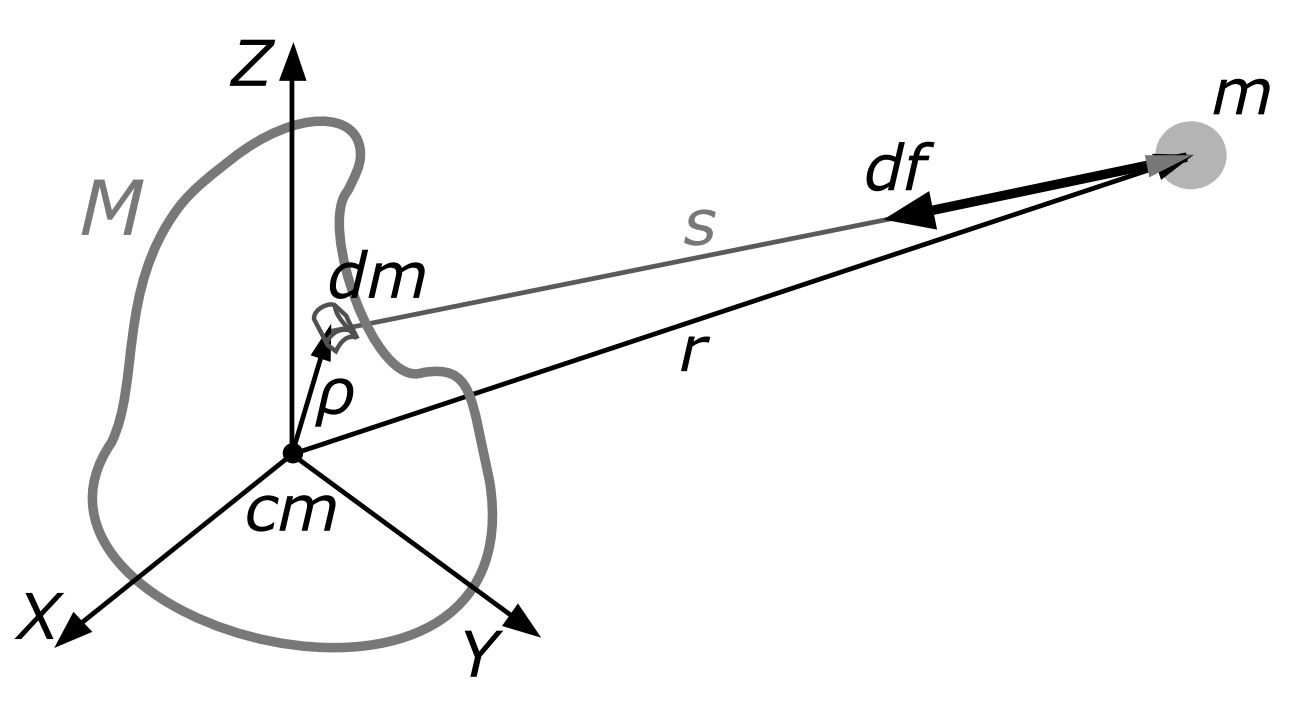
\includegraphics[width=2in]{figuras/geometriaref.png}
        \caption{Sistema de referência com origem no centro de massa do corpo $M$}
        Fonte: \cite{livro:aris1989}
        \label{fig:geometriaref}
\end{figure} 

Assim, o potencial gravitacional do elemento $dm$ sobre a massa $m$ é dado pela equação \ref{eq:8}, onde $s = \left|\left| \textbf{s} \right|\right|$ é a magnitude do vetor $\textbf{s}$. A aceleração da gravidade $\textbf{g}_{i}$ provocada pela massa $m_{i}$ é convertida na aceleração $d\textbf{g}$ do elemento $dm$, e quando substituído nas equações, retorna a equação \ref{eq:desgraça}.

\begin{equation}
    d\Phi =  \frac{Gdm}{s}
\label{eq:8}
\end{equation}

\begin{equation}
    \textbf{g} =  \int_{M} G\frac{\partial_{\frac{1}{s}}}{\partial \textbf{s}} dm = G \int_{M}\frac{\partial_{\frac{1}{s}}}{\partial \textbf{s}} dm
\label{eq:desgraça}
\end{equation}

Essa integral é tomada sobre toda a massa $M$, enquanto o vetor \textbf{s} varia em função da posição $\rho$ do elemento $dm$. É importante notar que a facilidade trazida anteriormente pelo potencial escalar $\Phi$ é eliminada pois a integral é de um campo vetorial devido ao gradiente ser calculado com respeito a $\textbf{s}$. Porém, quando consideramos a origem do referencial no $cm$ do corpo $M$, é possível utilizar a seguinte simplificação: se o $cm$ do corpo $M$ estiver suficientemente longe da massa $m$, a força gravitacional resultante atuará na direção do centro de massa, portanto, é possível trocar o gradiente com respeito ao vetor $\textbf{s}$ pelo gradiente com repeito ao vetor $\textbf{r}$, resultando na equação \ref{eq:sss}, que permite a simplificação da derivada, resultando na equação \ref{eq:adsd}.

\begin{equation}
    \textbf{g} = G \int_{M} \frac{\partial_{\frac{1}{s}}}{\partial \textbf{r}} dm
\label{eq:sss}
\end{equation}

\begin{equation}
    \textbf{g} = G \frac{\partial}{\partial \textbf{r}} \int_{M} \frac{1}{s}dm = \frac{\partial}{\partial \textbf{r}}G \int_{M} \frac{1}{s}dm
\label{eq:adsd}
\end{equation}

Assim, com a definição de potencial, o potencial gravitacional sobre a massa $m$ resultante do efeito do corpo $M$ é dada pela equação \ref{eq:122222}.

\begin{equation}
    \Phi = G \int_{M} \frac{1}{s}dm, \ onde \ \textbf{g} = \frac{\partial\Phi}{\partial \textbf{r}}
\label{eq:122222}
\end{equation}

\subsection{Força gravitacional para corpos axissimétricos}

A abordagem apresentada anteriormente é genérica. No caso de um corpo axissimétrico, é necessário assumir um modelo de corpo axissimétrico e também um sistema de coordenadas esféricas, como mostrado na figura \ref{fig:axis}, na qual, associado à massa pontual $m$, é definido um sistema de referência local, onde $\textbf{i}_{r}$ é um vetor diretor na direção radial, $\textbf{i}_{\phi}$ é um vetor diretor normal a $\textbf{i}_{r}$ (contido no plano $Z - \textbf{i}_{r}$ e apontando para baixo), e $\textbf{i}_{\theta}$ sendo paralelo ao plano equatorial e apontando no sentido horário do arco associado ao ângulo $\theta$, completando assim a tríade ortonomal dextrógira. Ainda na figura \ref{fig:axis}, existe um eixo $Z$ alinhado com o eixo de simetria do corpo $M$, sendo que os eixos $X$ e $Y$ estão contidos no seu plano equatorial (plano normal ao eixo de simetria, com máxima área de seção transversal do corpo). As coordenadas esféricas são escolhidas devido ao problema ter simetria axial, sendo que as coordenadas da massa $dm$ são distância radial $\rho$, colatitude $\beta$ e longitude $\lambda$, com as coordenadas análogas da massa $m$ sendo $r, \phi$ e $\theta$.

\begin{figure}[h]
        \centering
        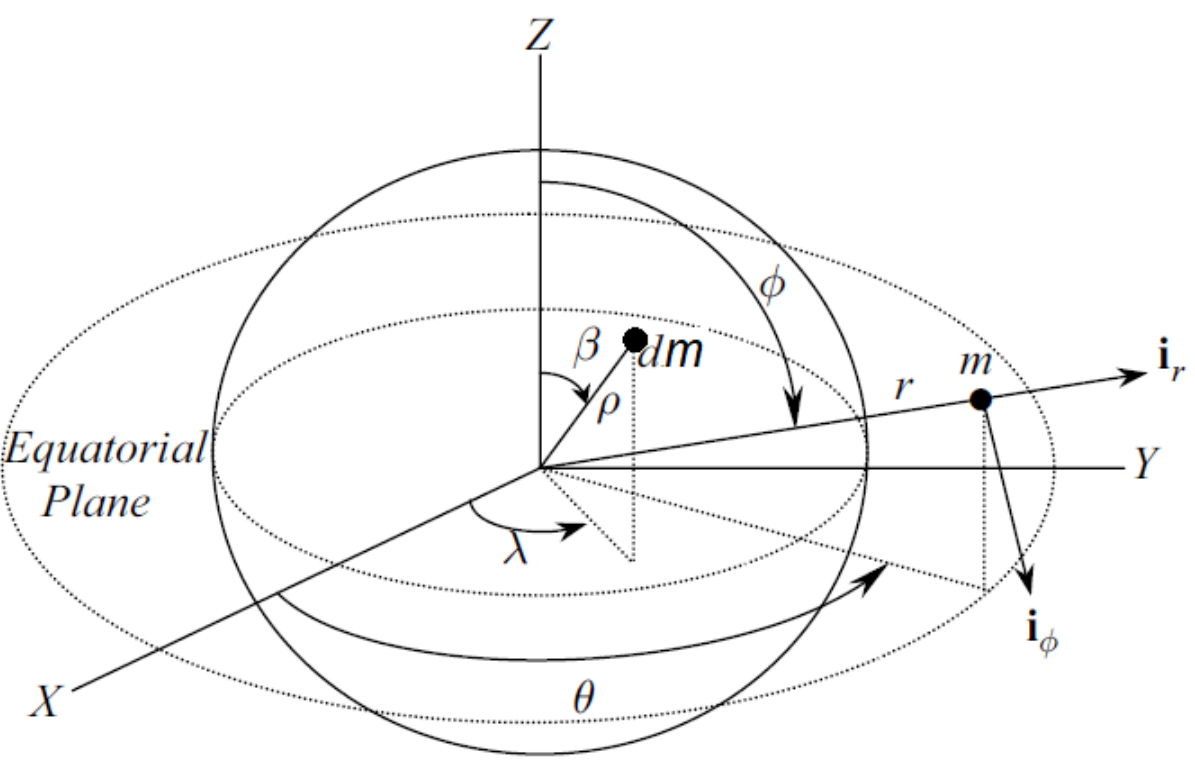
\includegraphics[width=3in]{figuras/axis.png}
        \caption{Modelo de corpo axissimétrico e sistema de coordenadas esféricas}
        \footnotesize Fonte: \cite{livro:andre}
        \label{fig:axis}
\end{figure} 

%%%%%%%%% Fim da aula 1

Para calcular o potencial gravitacional resultante, a distância $s$ é escrita com respeito ao sistema de coordenadas adotado, utilizando a lei dos cossenos. Substituindo nas equações anteriores, é obtida a equação \ref{eq:14}, a qual pode ser calculada tomando a expansão em série de polinômios de \textit{Legendre} (equação \ref{eq:15}), que é convergente para $\rho \leq r$, e possui forma compacta (pela relação recursiva) como mostrado na equação \ref{eq:16}.

\begin{equation}
    \Phi = \int_{M} \frac{G}  {\sqrt{\rho^{2} + r^{2} - 2\rho r cos(\gamma)}}   dm
\label{eq:14}
\end{equation}

\begin{equation}
    \frac{1}{\sqrt{\rho^{2} + r^{2} - 2\rho r cos(\gamma)}} = \frac{1}{r} \left\{   1 + \frac{\rho}{r} cos \gamma + \frac{1}{2} \left( \frac{\rho}{r} \right)^{2} (3cos^{2}\gamma - 1) +   \frac{1}{2} \left( \frac{\rho}{r} \right)^{3} (5cos^{3}\gamma - 3cos \gamma) + \dots                       \right\}
    \label{eq:15}
\end{equation}

\begin{equation}
    P_{n} (\nu) = \frac{(2n - 1)\nu P_{n-1} - (n-1) P_{n-2}(\nu) }       {n}
    \label{eq:16}
\end{equation}

Usando a notação de polinômios de Legendre, a expansão em série pode ser escrita como mostrado na equação \ref{eq:17}, fazendo com que o potencial gravitacional seja dado pela equação \ref{eq:18}.

\begin{equation}
    \frac{1}{\sqrt{\rho^{2} + r^{2} - 2\rho r cos(\gamma)}} = \frac{1}{r} \left\{  P_{0}cos \gamma) + \frac{\rho}{r}P_{1}(cos\gamma)   \left( \frac{\rho}{r} \right)^{2} P_{2} (cos\gamma) + \dots + 
 \left( \frac{\rho}{r} \right)^{n} P_{n} (cos\gamma) + \dots                      \right\}
    \label{eq:17}
\end{equation}

\begin{equation}
     \Phi =  \frac{G}{r}
     \int_{M}
     \sum\limits_{n=0}^{\mbox{$\infty$}}
     \left( \frac{\rho}{r}\right)^{n}
     P_{n} (cos\gamma) dm =  \frac{G}{r}
     \sum\limits_{n=0}^{\mbox{$\infty$}}
         \int_{M}
     \left( \frac{\rho}{r}\right)^{n}
     P_{n} (cos\gamma) dm
    \label{eq:18} 
\end{equation}

Para os termos $n = 0$ e $n = 1$, é simples resolver, pois para $n = 1$ a integral é nula devido a simetria, enquanto para $n = 0$ a resposta é dada simplesmente pela massa total, levando ao resultado do potencial gravitacional de uma distribuição esférica de massa, mostrada na equação \ref{eq:19}.

\begin{equation}
    \Phi_{0} = \frac{GM}{r}
    \label{eq:19}
\end{equation}

Para calcular os demais termos, o elemento de massa da integral precisa ser escrito em coordenadas polares, o que é feito a partir do elemento de volume neste sistema de coordenada, porém devido a hipótese do corpo axissimétrico, não há dependência de $D(\rho , \beta , \lambda)$ com a longitude $\lambda$, portanto, a função é tomada somente com respeito a $\rho$ e $\beta$, resultando na equação \ref{eq:21}.

\begin{equation}
    dm = D(\rho , \beta ) \rho^{2} sin \beta d\rho d \beta d \lambda
    \label{eq:21}
\end{equation}

É necessário ainda escrever o ângulo $\gamma$ nas coordenadas de $dm$ e $m$, assim, utilizando geometria esférica, $\gamma$ é dado pela equação \ref{eq:22}, porém, para o caso axissimétrico, $\gamma$ não depende da longitude de $dm$ e $m$, independendo assim de $\theta$ e $\lambda$, sendo válido o resultado mostrado na equação \ref{eq:23}.

\begin{equation}
    cos \gamma = cos \beta cos \phi + sin \beta sin\phi cos (\theta - \lambda)
    \label{eq:22}
\end{equation}

\begin{equation}
    P_{n} (cos \gamma) = P_{n} (cos \beta) P_{n}(cos\phi)
    \label{eq:23}
\end{equation}

Então, o potencial gravitacional do corpo axissimétrico é dado pela equação \ref{eq:24}.

\begin{equation}
    \Phi = \frac{GM}{r} + \frac{G}{r} \sum\limits_{n=2}^{\mbox{$\infty$}} \frac{P_{n}cos(\phi) }{r^{n}} 
    \int_{\rho = 0, \beta = 0, \lambda = 0}^{\rho = R_{e}, \beta = \pi, \lambda = 2\pi}
    \rho^{n}P_{n}(cos \beta)D(\rho , \beta ) \rho^{2} sin \beta d\rho d \beta d \lambda
    \label{eq:24}
\end{equation}

Uma solução consolidada para o problema envolve escrever o somatório como mostrado na equação \ref{eq:25}, que possui os coeficiente $A_{n}$ dados pela equação \ref{eq:26}.

\begin{equation}
    \Phi(r,\phi) = \frac{GM}{r} + \frac{~1}{r}\sum\limits_{n=2}^{\mbox{$\infty$}} \frac{A_{n} P_{n}cos(\phi) }{r^{n}} 
    \label{eq:25}
\end{equation}

\begin{equation}
    A_{n} = G \int_{\rho = 0, \beta = 0, \lambda = 0}^{\rho = R_{e}, \beta = \pi, \lambda = 2\pi}    \rho^{n+2}P_{n}(cos \beta)D(\rho , \beta )sin \beta d\rho d \beta d \lambda
    \label{eq:26}
\end{equation}

Na equação \ref{eq:27} é mostrada a expressão final do potencial gravitacional, na qual os coeficientes $A_{n}$ são trocados por $J_{n}$ (equação \ref{eq:28}), chamados de constantes de \textit{Jeffery}, que são parâmetros da expansão em harmônicos esféricos para o caso do corpo axissimétrico, além disso, aparece a variável $R_{e}$, que é o raio equatorial do planeta. É importante notar que cada planeta possui valores intrínsecos das constantes de Jeffery, e em geral, apenas os quatro primeiros termos da soma são necessários ($n = 2, 3, 4, 5 $), que diminuem conforme o grau $n$ aumenta. As contantes representam os desvios do campo gravitacional provocados pela variação da distribuição de massa quando comparado ao caso esférico. 

\begin{equation}
    \Phi(r,\phi) = \frac{GM}{r} \left\{ 1 - \sum\limits_{n=2}^{\mbox{$\infty$}} \left( \frac{R_{e}}{r}         \right)  J_{n} P_{n} (cos \phi) \right\}
    \label{eq:27}
\end{equation}

\begin{equation}
    J_{n} = -\frac{A_{n}}{GMR_{e}^{n}}
\label{eq:28}
\end{equation}

\subsection{Cálculo do campo gravitacional em coordenadas esféricas}

Em coordenadas esféricas, o cálculo do gradiente da função potencial é dado pela equação \ref{eq:29}.

\begin{equation}
    \frac{\partial \Phi}{\partial r} = \frac{\partial \Phi}{\partial r}i_{r} + \frac{1}{r} \frac{\partial \Phi}{\partial \phi}i_{\phi} + \frac{1}{r sin\phi}\frac{\partial \Phi}{\partial \theta}i_{\theta}
    \label{eq:29}
\end{equation}

\subsection{Raio de um planeta não esférico}

No caso do raio polar $R_{p}$ ser inferior ao raio equatorial $R_{e}$, é necessário definir uma representação confiável da superfície média do nível do mar, que serve como referência para determinar variações de altitude na superfície, sendo que pontos de grande variação de altitude podem gerar anomalias gravitacionais locais. O raio local $R$ é o raio que define a superfície de um elipsoide de referência, e é definido em função da latitude centrada no planeta. o raio local pode ser calculado pela equação \ref{eq:30}, onde $\epsilon$ é a elipticidade do planeta, que geralmente é um número de pequeno valor, fazendo com que a equação seja simplificada à equação \ref{eq:31}.

\begin{equation}
    R = R_{e} \left[ 1 - \frac{\epsilon}{2} (1-cos2\delta) + \frac{5\epsilon^{2}}{16}(1-cos4\delta) -\dots \right], \epsilon = 1- \frac{R_{p}}{R_{e}}
    \label{eq:30}
\end{equation}

\begin{equation}
    R \approx R_{e} \left(  1-\frac{\epsilon}{2}(1-cos2\delta) \right)
    \label{eq:31}
\end{equation}

\subsection{Vertical local}

A vertical local, definida como a direção normal à superfície de referência em determinado ponto, é medida a partir do elipsoide padrão tratado, e é utilizada para determinar pequenos desvios encontrados nas direções radial e vertical em planetas não esféricos. O desvio da vertical local $D$ é a diferença angular entre a vertical local real e a de aproximação esférica, sendo que para o caso elipsoidal, o desvio é dado pela expansão em série mostrada na equação \ref{eq:32}, na qual geralmente apenas os dois primeiros termos são considerados. 

\begin{equation}
    D = \epsilon sin 2\delta - \frac{\epsilon^{2}}{4}sin2\delta + 2\epsilon^{2} sin 2\delta sin^{2}\delta + \dots
    \label{eq:32}
\end{equation}
 
\subsection{Anomalias gravitacionais}

As anomalias gravitacionais são resultado da distribuição de massa real do planeta, que diferem do modelo axissimétrico, que fisicamente são superfícies equipotenciais (com contorno de potencial gravitacional constante). Quando maior precisão é necessária, os efeitos setoriais e tesserais (variações longitudinais na distribuição de massa e descrevem formas relacionadas com meridianos e paralelos) são considerados. Além disso, existem efeitos locais, como dito anteriormente. Quando é preciso levar em conta as pequenas variações gravitacionais, são utilizados os harmônicos esféricos, que são escritos a partir de funções de \textit{Legendre} ($P_{n}^{m}$) de ordem $m$ e grau $n$, que podem ser relacionados com os polinômios pela equação \ref{eq:33}, ou seja, os polinômios de Legendre são funções de Legendre de ordem zero. 


\begin{equation}
  P_{n} = P_{n}^{0}  
  \label{eq:33}
\end{equation}

Em um modelo gravitacional geral, os coeficientes dessa expansão são dados por $C_{n}^{m}$, sendo que as constantes de Jeffery são o negativo desses coeficientes de ordem zero do mesmo grau, como mostrado na equação \ref{eq:34}, sendo estes chamados de coeficientes harmônicos zonais. Todos os coeficientes com ordem $m \neq 0$, são associados com a distribuição não axissimétrica de massa, determinando a variação longitudinal da gravidade, sendo que os coeficientes de ordem $m = n$ são chamados de coeficientes harmônios setoriais, e os de ordem $m \neq n$ de coeficientes harmônicos tesserais. 

\begin{equation}
    J_{n} = -C_{n}^{0}
\label{eq:34}
\end{equation}


%%%%%%%%% Fim da aula 2

%%%%%%%%%%% AULA 3 - CODIGO 2

\section{Cálculo de propagação de órbita}
\subsection{Problema de N corpos}

O problema de $N$ corpos trata sobre o movimento de corpos suficientemente afastados, a ponto de serem considerados partículas. Assim, a única força de interação entre eles é a força gravitacional. Para esse problema, são assumidos $N$ corpos de massa $m_{i}$, sendo que somente as forças gravitacionais agem sobre o sistema, e a força gravitacional externa é nula. A variável $r_{i}$ representa a posição da $i-ézima$ partícula em um referencial inercial, enquanto  a posição da partícula $i$ com respeito à partícula $j$ é dado por $r_{ij} = r_{i} - r_{j}$, sendo a distância entre elas o módulo de $r_{ij}$. Aplicando a lei da atração gravitacional, é obtido um conjunto de $N$ equações diferenciais de segunda ordem, mostrados na equação \ref{eq:35}, onde cada equação possui 6 variáveis de estado devido a associação à derivada de segunda ordem de um vetor com 3 componentes. Portanto, existem $6N$ variáveis de estado, com $3N$ de posição de $3N$ de velocidade, e devido ao componente $\frac{1}{r_{ij}^{3}}$, as equações são não lineares.

\begin{equation}
    \frac{d^{2}r_{1}}{dt^{2}} = \sum\limits_{j=2}^{\mbox{N}}\frac{Gm_{j}}{r_{1j}^{3}} (r_{j} - r_{1}), \ 
     \frac{d^{2}r_{2}}{dt^{2}} = \sum\limits_{j=1}^{\mbox{N,$\neq j$}} \frac{Gm_{j}}{r_{2j}^{3}} (r_{j} - r_{2}), \ \dots, \ \frac{d^{2}r_{N}}{dt^{2}} = \sum\limits_{j=1}^{\mbox{N-1}}\frac{Gm_{j}}{r_{Nj}^{3}} (r_{j} - r_{N})
     \label{eq:35}
\end{equation} 

Para $N > 2$, a solução se torna um problema, sendo possível apenas por cálculo numérico. Assim, são aplicados conceitos de conservação de energia para ter um maior significado analítico. 

\subsection{Conservação da energia mecânica}

A energia mecânica é composta pelas energias potencial e cinética, portanto, para definir a energia mecânica, é necessário definir a energia potencial e a energia cinética. A energia potencial pode ser encontrada utilizando o potencial gravitacional mencionado anteriormente e também o conceito de energia potencial (que por definição, é o negativo do trabalho necessário para deslocar a partícula $m_{i}$ desde a situação em que ela está em contato com $m_{j}$, até a distância atual entre elas), que para $N$ corpos é dada pela equação \ref{eq:36}.

\begin{equation}
    V = -\frac{1}{2} \sum\limits_{i=1}^{\mbox{N}} \sum\limits_{j=1}^{\mbox{N, $ j\neq i $}} \frac{Gm_{i} m_{j}}{r_{ij}}
    \label{eq:36}
\end{equation}

A energia cinética é relacionada com o conceito de energia cinética para um sistema de partículas na qual cada partícula possui sua velocidade inercial $v_{i}$, assim, a energia cinética total do sistema é dada pela equação \ref{eq:37}.

\begin{equation}
    T = \sum\limits_{i=1}^{\mbox{N}} \frac{1}{2}m_{i}v_{i}^{2}
\label{eq:37}
\end{equation}

A energia mecânica então é dada por $E = T + V$, como mostrado na equação \ref{eq:38}, sendo que devido a força gravitacional ser conservativa, a energia mecânica é conservada. 

\begin{equation}
    E = \sum\limits_{i=1}^{\mbox{N}} \frac{1}{2}m_{i}v_{i}^{2} -\frac{1}{2} \sum\limits_{i=1}^{\mbox{N}} \sum\limits_{j=1}^{\mbox{N, $ j\neq i $}} \frac{Gm_{i}m_{j}}{r_{ij}} = constante 
    \label{eq:38}
\end{equation} 

\subsection{Conservação da quantidade de movimento angular e linear}

A quantidade de movimento angular do sistema é dada pela soma daquelas de todas as partículas, como mostrado na equação \ref{eq:39}, e possui valor constate devido a propriedade conservativa já que as forças internas que geram momento se cancelam. Assim, a quantidade de movimento angular total $H$ é outra integral de movimento, assim como $E$. Integral do movimento é o nome dado para uma propriedade que resulta em uma expressão algébrica igualada a uma constante. Dessa forma, juntando as integrais do movimento $E$ e $H$, a ordem do sistema de equações diferenciais é reduzida para $6N-4$.

\begin{equation}
    H = \sum\limits_{i=1}^{\mbox{N}} m_{i}r_{i} \times v_{i} = constante
    \label{eq:39}
\end{equation}

Para a quantidade de movimento linear, ocorre de maneira semelhante, sendo dado pela equação \ref{eq:40}. 

\begin{equation}
    P = \sum\limits_{i=1}^{\mbox{N}} m_{i}v_{i} = constante
    \label{eq:40}
\end{equation}

A quantidade de movimento linear total do sistema pode ser escrito em termos do centro de massa $CM$, assim, a velocidade do centro de massa do sistema de $N$ corpos é constante em um referencial inercial. Utilizando a definição da velocidade de centro de massa $v_{0}$, é possível obter outra integral do movimento, dada pela equação \ref{eq:41}, fazendo com que a ordem das equações diferenciais sejam reduzidas em 7 unidades.

\begin{equation}
    v_{0} = \frac{1}{M} \sum\limits_{i=1}^{\mbox{N}} m_{i}v_{i} = constante
    \label{eq:41}
\end{equation}

\subsection{Trajetória do centro de massa }

Utilizando a velocidade do $CM$ com a relação cinemática entre posição e velocidade é possível obter uma equação muito útil para a posição do $CM$, dada pela equação \ref{eq:42}, a qual mostra que uma constante vetorial $c$ é o próprio $CM$ quando $t = 0$, sendo assim outra integral de movimento. 

\begin{equation}
    r_{0} = \frac{1}{M} \sum\limits_{i=1}^{\mbox{N}} m_{i}r_{i} = c+v_{0}t
\label{eq:42}
\end{equation}

Portanto, utilizando as relações das constantes $v_{0}, c, H, E$, o sistema de equações diferenciais passa a ser restringido por 10 equações algébricas, o que reduz sua ordem para 6N-10, portanto, no caso de dois corpos, ainda restam duas equações diferenciais no sistema. 

\subsection{Problema de 2 corpos}

Para dois corpos, se obtém a equação diferencial homogênea \ref{eq:43}, na qual $\mu = G(m_{1} + m_{2})$ e $r = r_{21} = r_{2} - r_{1}$.

\begin{equation}
    \frac{d^{2} r}{dt^{2}} + \frac{\mu r}{r^{3}} = 0
    \label{eq:43}
\end{equation}

Para resolver essa equação, são utilizados os conceitos de integral de movimento. Inicialmente, se procura uma propriedade para a quantidade de movimento angular. Usando o produto vetorial por $r$ em ambos os lados da equação anterior e usando o vetor velocidade junto da identidade $r \times r = 0$, é obtida a equação \ref{eq:44}, que é o vetor quantidade de movimento angular específica, que tem unidade de quantidade de movimento angular por unidade de massa $h = r \times v$, na qual $h$ é a quantidade de movimento angular por unidade de massa do movimento relativo de $m_{2}$ com respeito a $m_{1}$ e possui valor constante, ou seja, a quantidade de movimento angular específica é conservada, fazendo com que a trajetória definida pelos vetores $r$ e $v$ seja plana. 

\begin{equation}
    \frac{dr \times v}{dt} = 0
    \label{eq:44}
\end{equation}

Em coordenadas polares (distância radial $r$ e ângulo polar $\theta$), o vetor quantidade de movimento angular específica é dado pela equação \ref{eq:45}, onde $i_r$ e $i_{\theta}$ são os vetores unitários dessas coordenadas, e $k = i_{r} \times i_{\theta}$ é o vetor unitário normal ao plano do movimento. 
\begin{equation}
    h = ri_{r} \times \left( \frac{dr}{dt}_{r} + r\frac{d\theta}{dt}i_{\theta}  \right) = r^{2}\frac{d\theta}{dt}i_{r} \times i_{\theta}
  \label{eq:45}  
\end{equation}

Assim, a magnitude da quantidade de movimento angular específica é dada pela equação \ref{eq:46}, que está relacionada com a segunda Lei de Kepler, que define a velocidade areolar, dada pela equação \ref{eq:47}, que afirma que a velocidade areolar é constante. Além disso, essa propriedade é válida para qualquer solução do problema de dois corpos, não apenas a trajetória elíptica mencionada nas Leis de Kepler.

\begin{equation}
    h = r^{2}\Dot{\theta} = constante
    \label{eq:46}
\end{equation}

\begin{equation}
    \Dot{A} = \frac{1}{2}r^{2}\Dot{\theta}
    \label{eq:47}
\end{equation}

\subsection{Excentricidade}

A equação \ref{eq:48} mostra o vetor excentricidade, que é obtido a partir de uma integral de movimento dada pela equação \ref{eq:49}.

\begin{equation}
e = \frac{1}{\mu}v \times h - \frac{\textbf{r}}{r}
\label{eq:48}
\end{equation}

\begin{equation}
    v \times h - \mu\frac{\textbf{r}}{r} = constante
    \label{eq:49}
\end{equation}

A excentricidade da trajetória é dada pela equação \ref{eq:50}, a partir das quais se definem duas constantes, o parâmetro $p$ e o semi eixo maior $a$, dados pela equação \ref{eq:51}, e relacionados pela equação \ref{eq:52}. Pela definição de $a$, outra integral do movimento é obtida, mostrada na equação \ref{eq:53}, a qual mostra a energia mecânica específica do movimento relativo ($\epsilon$) em função da energia cinética do movimento relativo por unidade de massa ($v^{2}/2$) e da energia potencial por unidade de massa do movimento relativo ($-\mu /r$).

\begin{equation}
    1-e^{2} = \frac{2h^{2}}{\mu r} - \frac{v^{2} h^{2}}{\mu^{2}} = \frac{h^{2}}{\mu} \left(    \frac{2}{r} - \frac{v^{2}}{\mu} \right)
    \label{eq:50}
\end{equation}

\begin{equation}
    p = \frac{h^{2}}{\mu}, \ \frac{1}{a} = \frac{2}{r} - \frac{v^{2}}{\mu}
    \label{eq:51}
\end{equation}

\begin{equation}
    p = (1-e^{2})a
    \label{eq:52}
\end{equation}

\begin{equation}
    \epsilon = \frac{v^{2}}{2} - \frac{\mu}{r}
    \label{eq:53}
\end{equation}

Algumas conclusões são obtidas analisando as equações. Uma órbita limitada é aquela na qual a energia cinética relativa por unidade de massa é menor que a magnitude da energia potencial específica, ou seja, $\epsilon < 0$ ou $a > 0$. Uma trajetória de escape é aquela na qual a energia relativa específica é maior ou igual à energia potencial específica, ou seja, $\epsilon < 0 $ ou $a<0$. A excentricidade também pode ser escrita em termos de $p$ e $a$, como mostrado na equação \ref{eq:54}.

\begin{equation}
    e = \sqrt{1-\frac{p}{a}}
    \label{eq:54}
\end{equation}

\subsection{Equação de órbita: geometria das soluções de problemas de dois corpos}

Para determinar a geometria das soluções, é necessário definir a projeção do vetor posição sobre a direção inercial definida por $e$, o que pode ser feito a partir do produto escalar entre o vetor $\mu e$ e a posição $r$. Realizando isso, é obtida a equação \ref{eq:55}, que pode ser representada em coordenadas polares, resultando na equação \ref{eq:56}, que define a geometria das trajetórias, sendo chamada de equação de órbita. Qualquer trajetória do problema de dois corpos deve satisfazê-la, sendo caracterizada pela anomalia verdadeira. 

\begin{equation}
e \cdot \textbf{r} + r = \frac{h^{2}}{\mu}
    \label{eq:55}
\end{equation}

\begin{equation}
    r = \frac{p}{1+ecos\theta}
\label{eq:56}
\end{equation}

É importante também definir a decomposição do vetor velocidade, dada pela equação \ref{eq:velocidade}, que possui duas componentes, dados pela equação \ref{eq:Ve2}. É possível ainda obter o ângulo de trajetória $\phi$ a partir da equação \ref{eq:v3}.


\begin{equation}
    \textbf{v} = vcos\phi i_{\theta} + vsin\phi i_{r}
    \label{eq:velocidade}
\end{equation}

\begin{equation}
    cos (\phi) = \frac{\mu (1+ecos\theta)}{hv}, \ sin (\phi) = \frac{\mu e sin\theta}{hv}
    \label{eq:Ve2}
\end{equation}

\begin{equation}
    tan\phi = \frac{esin\theta}{1+ecos\theta}
    \label{eq:v3}
\end{equation}


\subsection{Órbitas elípticas, parabólicas e hiperbólicas}

Para a órbita elíptica, as distâncias de periastro $r_{p}$ e apoastro $r_{a}$ são calculadas quando $\theta = 0$ e $\theta = \pi$, sendo válidas quando $e<1$, obtendo assim as equações mostradas em \ref{eq:57}, que são válidas para $a>0$, obtendo assim uma órbita elíptica. Pode-se verificar também que para $\theta = \frac{\pi}{2}$, p é a distância normal da linha dos apsides até a trajetória medida a partir do foco. Existe também um vetor que aponta desde o foco até a órbita ao longo da linha de apsides, ou seja, do foco até o periastro. Esse vetor é dado pela equação \ref{eq: 58}.

\begin{equation}
    r_{p} = (1-e)a, \ r_{a} = (1+e)a
    \label{eq:57}
\end{equation}

\begin{equation}
    q = \left(  \frac{1}{e} - 1\right)a
    \label{eq: 58}
\end{equation}

Para a órbita parabólica ($e = 1$ devido ao periastro para $\theta = 0$), é obtida a equação \ref{eq:59}, que mostra que a órbita é de escape, com apoastro indefinido.

\begin{equation}
    r_{p} = \frac{p}{2}, \ q = \frac{p}{2}
    \label{eq:59}
\end{equation}

Para a órbita hiperbólica ($e >1$), o periastro novamente é definido para $theta = 0$, resultando na equação \ref{eq:60}.

\begin{equation}
    r_{p} = -a(e-1), \ q = -a \left( 1-\frac{1}{e}\right)
    \label{eq:60}
\end{equation}

\subsection{Coeficientes de Lagrange}

Os coeficientes de Lagrange servem para determinar a posição e velocidade a partir de uma condição inicial de posição e velocidade do referencial perifocal (definido ao longo dos eixos gerados pelos vetores unitários $i_e$ e $i_{p}$, sendo o plano definido por estes o plano orbital, e tendo $i_{h}$ normal à órbita) em qualquer órbita do problema de dois corpos. A velocidade escrita no sistema perifocal é dada pela equação \ref{eq:61}, enquanto a posição é dada pela equação \ref{eq:62}.


\begin{equation}
    \textbf{v} = vsin\phi i_{r} + vcos\phi i_{\theta}
    \label{eq:61}
\end{equation}
\begin{equation}
    \textbf{r} = rcos\theta i_{e} + r sin \theta i_{p}
    \label{eq:62}
\end{equation}

Obtendo uma transformação da posição e velocidade no sistema perifocal a partir de condições iniciais conhecidas e determinando seus valores para uma anomalia verdadeira $\theta$ genérica, são definidos os coeficientes de Lagrange. Após equacionar utilizando matrizes e também as definições descritas anteriormente, é encontrado uma matriz escrita no sistema perifocal, sendo seus elementos os coeficientes de Lagrange. A matriz é mostrada na equação \ref{eq:63}, junto de seus coeficientes (equação \ref{eq:64}).

\begin{equation}
\left\{\begin{array}{l}
\textbf{r} \\
\textbf{v} \end{array}\right\} = 
\left[\begin{array}{ll}
f & g \\
\Dot{f} & \Dot{g}
\end{array}\right] 
\left\{\begin{array}{l}
\textbf{$r_{0}$} \\
\textbf{$v_{0}$} 
\end{array}\right\}
\label{eq:63}
\end{equation}


\begin{equation}
\begin{split}
\begin{array}{l}
f \equiv 1 +\frac{r}{p}[cos(\theta - \theta_{0}) -1]\\ \\
g \equiv \frac{rr_{0}}{h}sin(\theta - \theta_{0})  \\ \\
\Dot{f} \equiv \frac{df}{dt} =  -\frac{h}{p^{2}}[sin(\theta - \theta_{0}) + e(sin\theta -sin \theta_{0})]\\ \\
\Dot{g} \equiv \frac{dg}{dt} = 1+ \frac{r_{0}}{p}[cos(\theta - \theta_{0}) -1]  
\end{array}
\label{eq:64}
\end{split}
\end{equation}

Assim, o objetivo é encontrar a posição e velocidade no referencial perifocal associadas a uma anomalia verdadeira $\theta$ genérica a partir de uma condição inicial $v_{0}$ e $r_{0}$ associada a uma anomalia verdadeira inicial $\theta_{0}$. Os coeficientes dependem das constantes $e, p$ e $h$. Essa matriz também é chamada de matriz de transição de estado.  

\subsection{Equação diferencial para propagação da anomalia verdadeira}

A equação \ref{eq:65} é uma equação diferencial que geralmente é resolvida por métodos numéricos, porém pode ter soluções analíticas que dependem do tipo de órbita. Essa equação serve para relacionar a propagação de órbita com caraterísticas temporais. 

\begin{equation}
 \frac{d\theta}{(1+ecos\theta)^{2}} = \sqrt{\frac{\mu}{p^{3}}dt}
 \label{eq:65}
\end{equation}

\subsection{Propagação de órbita elíptica}

Para uma órbita elíptica, com $e = 0 \leq e <1$ e de acordo com a relação $p = (1-e)^{2}a$, a equação \ref{eq:65} é reescrita como mostrado na equação \ref{eq:66}.

\begin{equation}
    \frac{(1-e^{2})^{\frac{3}{2}}d\theta}{(1+ecos\theta)^{2}} = \sqrt{\frac{\mu}{a^{3}}dt}
    \label{eq:66}
\end{equation}

Para uma órbita circular, a equação seria como mostrada na equação \ref{eq:67}, sendo essa equação correspondente a um movimento circular uniforme com velocidade angular $n$, que é chamada de movimento médio, que é a velocidade angular constante em uma órbita circular de raio $a$ sobrescrita à trajetória elíptica de semi eixo maior $a$. 

\begin{equation}
    \frac{d\theta}{dt} = \sqrt{\frac{\mu}{a^{3}}}, \ n = \sqrt{\frac{\mu}{a^{3}}}
    \label{eq:67}
\end{equation}

A partir disso, é definida a anomalia excêntrica $E$, que é igual à anomalia verdadeira quando $\theta = n\pi$ para $n$ inteiro, assim, para calcular $\theta$ em qualquer instante de tempo, é necessário definir $E$. 

As equações \ref{eq:Ecos} e \ref{eq:Esen} expressam o cosseno  e seno do angulo $E$, a partir dos quais se determina a anomalia excêntrica sem ambiguidade do quadrante. Utilizando essas equações, se obtém a equação diferencial para propagação da anomalia excêntrica, dada pela equação \ref{eq:68}.

\begin{equation}
    cos E = \frac{e+cos\theta}{1+ecos\theta}
    \label{eq:Ecos}
\end{equation}

\begin{equation}
    sin E = \frac{\sqrt{1-e^{2} sin \theta}}{1+ecos\theta}
    \label{eq:Esen}
\end{equation}


\begin{equation}
    (1-ecosE)dE = ndt
    \label{eq:68}
\end{equation}

Para resolver a equação \ref{eq:68}, é necessário integrá-la desde um tempo inicial até um tempo final, sendo este inicial uma das integrais de movimento. Assim, a integral é feita desde o tempo de periastro da órbita até um tempo qualquer, sendo que no instante inicial $\theta = E = 0$, que é a definição de periastro. Dessa forma, é obtida a equação \ref{eq:69}, chamada equação de \textit{Kepler} para órbitas elípticas, sendo o termo a direita da equação chamado de anomalia média $M$.

\begin{equation}
    E - esinE = n(t -\tau)
    \label{eq:69}
\end{equation}

Essa equação parece simples, porém possui resolução analítica complexa que precisa de métodos de variáveis complexas. Da equação de Kepler, é possível obter o período orbital, que é o tempo gasto para completar uma volta completa na órbita, dado pela equação \ref{eq:70}.

\begin{equation}
    T = \frac{2\pi}{n}
    \label{eq:70}
\end{equation}

Com essa equação, é possível concluir que para órbitas baixas o período é curto, enquanto para órbitas altas possuem período maior.

Assim, a partir da equação de Kepler, é possível propagar a anomalia excêntrica em função do tempo usando métodos numéricos. Quando encontrada a anomalia excêntrica, é possível determinar a anomalia verdadeira, porém para não ocorrerem problemas de ambiguidade, é interessante se avaliar de outras formas, como encontrando uma relação envolvendo tangente, dada pela equação \ref{eq:71}.

\begin{equation}
    tan\frac{\theta}{2} = \sqrt{\frac{1+e}{1-e}}tan\frac{E}{2}
    \label{eq:71}
\end{equation}
Por fim, para a propagação da órbita elíptica no referencial perifocal, é necessário calcular os coeficientes de Lagrange associados à anomalia verdadeira $\theta$, podendo assim determinar os vetores posição e velocidade.

%%%%%%%%%%% FIM AULA 5

\subsection{Propagação de órbita hiperbólica}

Para propagação de órbita hiperbólica, com $e >1$, a equação \ref{eq:63} é reescrita como a equação \ref{eq:72}, a qual pode ser resolvida por integração desde o tempo de periastro até um tempo qualquer no lado esquerdo e no lado direito desde $\theta = 0$ até uma anomalia verdadeira genérica $\theta' = \theta$.

\begin{equation}
\sqrt{\frac{\mu}{p^{3}}}dt = \frac{d\theta}{(1+ecos\theta)^{2}}
    \label{eq:72}
\end{equation}

Assim, é obtida a equação \ref{eq:73}, sendo $M_{h}$ definido como anomalia média hiperbólica, a parti da qual se define a anomalia hiperbólica $H$, que é utilizada na equação de Kepler para a hipérbole, dada na equação \ref{eq:74}.

\begin{equation}
M_{h} = (e^{2}-1)^{\frac{3}{2}}\sqrt{\frac{\mu}{p^{3}} (t-\tau)}
    \label{eq:73}
\end{equation}
\begin{equation}
    M_{h} = esinhH-H
    \label{eq:74}
\end{equation}

É visto que essa equação é análoga à equação de Kepler da elipse, porém a anomalia excêntrica é trocada pela hiperbólica, e a função seno é trocada pela função seno hiperbólico. Também não existe solução analítica simples, sendo necessário o uso de métodos numéricos. Primeiro é calculada a anomalia média hiperbólica, depois resolve-se a equação de Kepler encontrando a anomalia hiperbólica $H$, então calcula-se a anomalia verdadeira $\theta$, determina-se os coeficientes de Lagrange e assim são definidos os vetores posição e velocidade, no referencial perifocal, a partir da matriz de transição de estado e condições iniciais. Para encontrar a anomalia verdadeira, é necessário converter a anomalia hiperbólica, o que é feito a partir da equação \ref{eq:75}.

\begin{equation}
    tan\frac{\theta}{2} = \sqrt{\frac{e+1}{e-1}}tanh\frac{H}{2}
    \label{eq:75}
\end{equation}

\subsection{Propagação de órbita parabólica}

Para a propagação de órbita parabólica, a equação \ref{eq:63} com $e = 1$ se torna a equação \ref{eq:76}, que quando integrada da mesma forma que anteriormente, retorna a equação \ref{eq:77}, chamada de equação de \textit{Barker}.

\begin{equation}
    \sqrt{\frac{\mu}{p^{3}}}dt = \frac{d\theta}{(1+cos\theta)^{2}}
   \label{eq:76} 
\end{equation}

\begin{equation}
    \sqrt{\frac{\mu}{p^{3}}}(t-\tau) = \frac{1}{2}tan\frac{\theta}{2}+\frac{1}{6}tan^{3}\frac{\theta}{2}
    \label{eq:77}
\end{equation}

Como não há um conceito equivalente de anomalia excêntrica para a parábola, a forma de encontrar a anomalia verdadeira é dada pela equação \ref{eq:78}, que precisa ser resolvida para a variável $\alpha$, dada pela equação \ref{eq:79}.

\begin{equation}
    tan^{3} \frac{\theta}{2} + 3tan\frac{\theta}{2}-6\sqrt{\frac{\mu}{p^{3}}}(t-\tau) = 0
    \label{eq:78}
\end{equation}

\begin{equation}
    \alpha^{3}+3\alpha-6M_{p} = 0, tan\frac{\theta}{2} = \alpha
    \label{eq:79}
\end{equation}

Sendo $M_{p}$ a anomalia média parabólica, dada pela equação \ref{eq:80}.

\begin{equation}
    M_{p} = \sqrt{\frac{\mu}{p^{3}}}(t-\tau)
    \label{eq:80}
\end{equation}

Assim, a única solução real é dada pela equação \ref{eq:81}. É possível notar que enquanto a órbita elíptica tem energia relativa negativa, na qual os dois primários estão ligados gravitacionalmente, uma órbita hiperbólica possui energia relativa positiva, o que consiste em uma trajetória de escape do campo gravitacional de um planeta. Entre ambos, está a órbita parabólica, com energia relativa nula. A órbita parabólica determina a mínima energia para escapar da ação gravitacional de um planeta, sendo usada para estimar o requisito de combustível mínimo de uma missão interplanetária. 

\begin{equation}
    tan\frac{\theta}{2} = \left( 3M_{p} + \sqrt{1+9M_{p}^{2}}     \right)^{\frac{1}{3}}-\left( 3M_{p} + \sqrt{1+9M_{p}^{2} }    \right)^{\frac{1}{3}}
    \label{eq:81}
\end{equation}

\section{Cálculo de determinação de órbita}

\subsection{Referencial Celeste e elementos orbitais}
A órbita na qual uma massa $m_{2}$ orbita uma massa $m_{1}$ em um problema de dois corpos é plana, sendo caracterizada no plano orbital por um conjunto de três parâmetros, que podem ser escolhidos dentre várias opções. Mesmo apenas três parâmetros sendo suficientes para caracterizar a órbita no plano orbital, a solução do movimento relativo no problema de dois corpos depende de 6 integrais do movimento, ou seja, 6 parâmetros que caracterizam a trajetória para um observador fora do plano orbital. Os vetores posição inicial e velocidade inicial consistem num conjunto de 6 parâmetros, sendo um conjunto de elementos orbitais, porém não é um conjunto muito prático e intuitivo, pois não existe um referencial mais geral, assim, para determinar uma órbita para um observador genérico fora do plano geral, é definido um referencial com respeito ao qual qualquer órbita ao redor do corpo $m_{1}$ possa ser descrita, sendo que tal referencial precisa ser inercial e possuir eixos com direções bem definidas devido ao problema de ambiguidade.

O referencial Celeste terrestre, definido na figura \ref{fig:CELESTE}, possui origem no centro de massa da Terra, e não é exatamente inercial devido à aceleração do centro de massa proveniente do movimento orbital ao redor do Sol, porém pode ser considerado inercial. Esse referencial possui sua principal orientação dada pelo eixo $X$, que aponta na direção do equinócio vernal (representa o primeiro dia da primavera no hemisfério norte, ou outono no hemisfério sul, sendo aproximadamente o dia 21 de março), que ocorre ao meio dia e está orientado ao longo da interseção dos planos "equador celeste" e "eclíptica". O equador celeste é o prolongamento do plano equatorial terrestre, enquanto a eclíptica é o plano da órbita da Terra ao redor do Sol.

\begin{figure}[h]
        \centering
        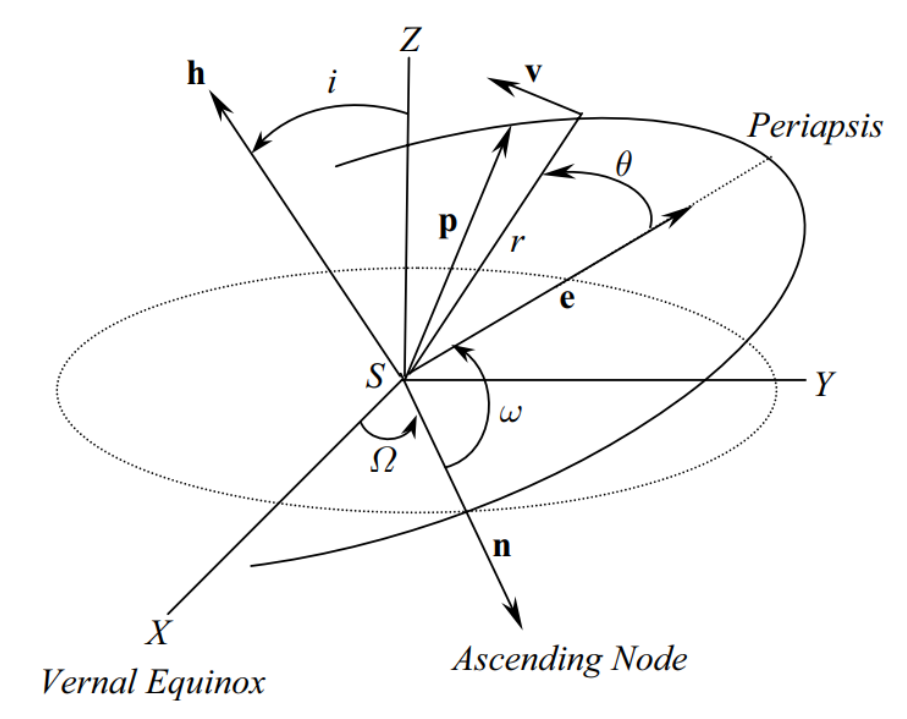
\includegraphics[width=3in]{figuras/celeste.png}
        \caption{Referencial celeste e ângulos de Euler do plano orbital}
        \footnotesize Fonte: \cite{livro:andre}
        \label{fig:CELESTE}
\end{figure} 


O eixo $Z$ depende do tipo de órbita avaliada, no caso de órbitas próximas da Terra, o eixo $Z$ costuma ser definido como apontando no sentido do polo norte celeste, que é o prolongamento do polo norte da Terra. No caso de órbitas de transferência interplanetária, o eixo é definido como apontando para o polo norte da eclíptica. 

O eixo $Y$ completa o sistema cartesiano de mão direita, quando $Z$ está para o polo norte celeste, $Y$ é definido tal que o plano $XY$ seja o equador celeste. Quando $Z$ está para o polo norte da eclíptica, $Y$ é definido tal que o plano $XY$ seja o plano da eclíptica. A definição usada é aquela na qual $Z$ aponta na direção do polo norte da eclíptica. 

Com o referencial definido, é possível referenciar uma órbita qualquer em relação a ele, o que pode ser feito por ângulos de Euler, geralmente na sequência de rotações 313, mostrada na figura \ref{fig:CELESTE}, onde o vetor \textbf{n} é unitário e está alinhado com a linha dos nodos (sendo essa a interseção do plano orbital com o plano $XY$ do referencial celeste), e possui direção apontando para o local onde a órbita cruza o plano celeste vindo do polo sul em direção ao norte. O primeiro ângulo de Euler é o $\Omega$ (longitude do nodo ascendente), sendo a rotação no sentido da mão direita em torno do eixo $Z$, fazendo $X$ girar até encontrar \textbf{n}. O segundo ângulo de Euler é o \textit{i} (inclinação da órbita), sendo a rotação no sentido positivo da mão direita em torno de \textbf{n} tal que o plano $XY$ gire até encontrar o plano da órbita. O terceiro ângulo é o $\omega$ (argumento de periastro), também no sentido positivo da mão direita, sendo a rotação feita em torno do vetor \textbf{h} da órbita com magnitude tal que o vetor \textbf{n} seja rotacionado até encontrar o vetor \textbf{e}. Após as rotações, o sistema de referência resultante é o perifocal, que tem os eixos $x$ e $y$ alinhados aos vetores \textbf{e} e \textbf{p}, respectivamente, e $z$ dirigido ao longo do vetor \textbf{h}. Os ângulos de Euler possuem singularidade na segunda rotação $i$ para valores de zero ou $\pi$ rad. Assim, órbitas equatoriais não podem ser descritas usando os parâmetros $\Omega$, $i$ e $\omega$. Além disso, quando a excentricidade é nula, o periastro é indeterminado, não sendo possível obter $\omega$.

Quando os parâmetros $\Omega$, $i$ e $\omega$ existem, eles constituem 3 elementos orbitais, que juntos de 3 parâmetros no plano orbital foram um conjunto de 6 elementos orbitais que caracterizam completamente uma órbita no espaço tridimensional. 


\subsection{Coordenadas esféricas Celestes e Horizonte Local}

Para problemas com simetria esférica, podem ser utilizadas coordenadas esféricas, como mostrado na figura \ref{fig:ESFCEL}. Para uma órbita genérica do problema de dois corpos com uma massa $m_{2}$ com posição $O$ em dado instante de tempo, a origem $S$ do referencial está no centro da massa $m_{1}$. As coordenadas esféricas são a distância radial $r$ entre $S$ e $O$, o ângulo $\delta$ entre o segmento $SO$ e o plano $XY$ do referencial celeste (chamado de latitude celeste ou declinação, sendo positiva quando medida acima deste plano), e o ângulo $\lambda$ entre a projeção do segmento $SO$ sobre o plano $XY$ e o eixo $X$ (chamado de longitude celeste, sendo positivo na direção leste). Esse referencial serve para definir um horizonte local ao longo da órbita, sendo possível definir os eixos de diversas formas, sendo que na figura \ref{fig:ESFCEL} o eixo $x$ está alinhado com o radial $SO$ com direção positiva afastando-se de $O$. O eixo $z$ é normal a $x$ e aponta para o norte, enquanto o eixo $y$ completa o sistema de referência de mão direita, que aponta para o leste. Os eixos $y$ e $z$ formam o plano horizontal local, enquanto $x$ aponta para cima em relação à superfície do astro, sendo por essa sequencia de eixos $x (up)$, $y (east)$ e $z (north)$, chamado de \textbf{UEN}. A orientação do referencial horizontal local é obtida a partir de duas rotações elementares com respeito ao celeste, sendo a primeira pelo ângulo $\lambda$ em torno do eixo $Z$ do sistema celeste no sentido positivo da mão direita (com o eixo $y$ resultante apontando na direção leste), e a segunda pelo ângulo $\delta$ em torno do eixo $y$ (leste) no sentido negativo da mão direita. 

\begin{figure}[h]
        \centering
        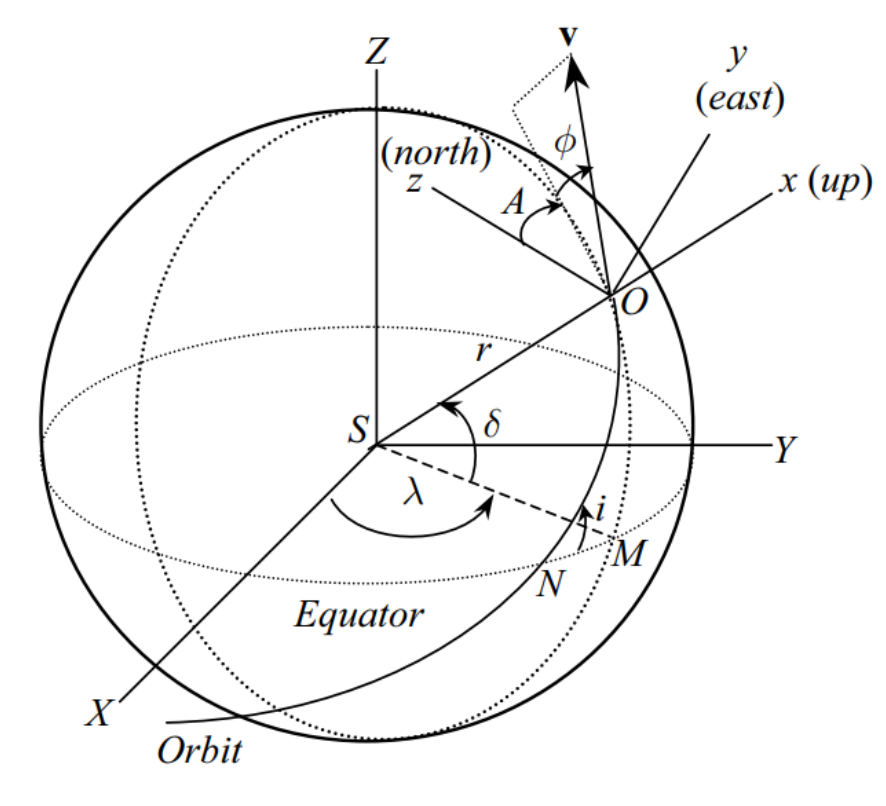
\includegraphics[width=3in]{figuras/ESFCEL.png}
        \caption{Coordenadas celestes esféricas e horizonte local}
        \footnotesize Fonte: \cite{livro:andre}
        \label{fig:ESFCEL}
\end{figure} 

\subsection{Equações de navegação: velocidade e posição}

A principal utilidade do referencial horizontal local é escrever o vetor velocidade, que é dado em termos de $v$ (magnitude), $\phi$ (ângulo de trajetória) e $A$ (azimute de velocidade), e pode ser escrito como mostrado na equação \ref{eq:VELOCIDADEHORIZONTE}. A velocidade inercial escrita no referencial celeste é dada pela equação \ref{eq:VELOCIDADEHORIZONTE2}. A relação entre velocidade inercial escrita nos referenciais horizontal local e celeste é dada pela equação \ref{eq:VELOCIDADEHORIZONTE3}.

\begin{equation}
Vhl =  
\left[\begin{array}{l}
v_{x} \\
v_{y}  \\
v_{z} 
\end{array}\right] = 
\left[\begin{array}{l}
v sin\phi\\
v cos\phi sin A \\
v cos\phi cos A
\end{array}\right]
\label{eq:VELOCIDADEHORIZONTE}
\end{equation}

\begin{equation}
Vc =
\left[\begin{array}{l}
v_{X} \\
v_{Y}  \\
v_{Z} 
\end{array}\right] = 
\left[\begin{array}{lll}
cos \delta cos\lambda & -sin\lambda & -cos\lambda sin\delta \\
cos \delta sin\lambda & cos\lambda & -sin\delta sin\lambda \\
sin \delta & 0 & cos\delta
\end{array}\right]
\left[\begin{array}{l}
v sin\phi\\
v cos\phi sin A \\
v cos\phi cos A
\end{array}\right]
\label{eq:VELOCIDADEHORIZONTE2}
\end{equation}

\begin{equation}
\left[\begin{array}{l}
v_{X} \\
v_{Y}  \\
v_{Z} 
\end{array}\right] = 
\left[\begin{array}{l}
v (sin\phi cos\delta cos\lambda - cos\phi sin A sin\lambda - cos\phi cos A sin \delta cos\lambda)\\
v (sin\phi cos\delta sin\lambda + cos\phi sin A cos\lambda - cos\phi cos A sin \delta sin\lambda)\\
v (sin\phi sin \delta + cos\phi cos A cos \delta)
\end{array}\right]
\label{eq:VELOCIDADEHORIZONTE3}
\end{equation}

Da mesma forma para o vetor posição, tem-se as equações \ref{eq:POSICAO1}, \ref{eq:POSICAO2} e \ref{eq:POSICAO3}.

\begin{equation}
Rhl =  
\left[\begin{array}{l}
r \\
0  \\
0 
\end{array}\right]
\label{eq:POSICAO1}
\end{equation}

\begin{equation}
Rc =
\left[\begin{array}{l}
X \\
Y  \\
Z 
\end{array}\right] = 
\left[\begin{array}{lll}
cos \delta cos\lambda & -sin\lambda & -cos\lambda sin\delta \\
cos \delta sin\lambda & cos\lambda & -sin\delta sin\lambda \\
sin \delta & 0 & cos\delta
\end{array}\right]
\left[\begin{array}{l}
r \\
0  \\
0 
\end{array}\right]
\label{eq:POSICAO2}
\end{equation}

\begin{equation}
\left[\begin{array}{l}
X \\
Y  \\
Z 
\end{array}\right] = 
\left[\begin{array}{l}
r cos\delta cos\lambda\\
r cos\delta sin\lambda\\
r sin\delta
\end{array}\right]
\label{eq:POSICAO3}
\end{equation}

\subsection{Referencial fixo ao planeta}

O referencial fixo ao planeta, mostrado na figura \ref{fig:PLANETAZUM}, é útil pois o referencial celeste possui seus eixos $X$ e $Y$ referenciados a estrelas, enquanto o referencial local horizontal move-se junto do corpo que realiza a órbita, sendo assim, é necessário um referencial que tem como referencia o planeta, o qual é girante. Assim, define-se o referencial centrado no planeta e fixo ao mesmo, sendo que no caso da Terra é chamado de earth centered, earth fixed (ECEF) e possui a origem sendo o centro de massa do planeta. O eixo $Z'$ é alinhado ao eixo polar celeste, sendo coincidente com o eixo $Z$ do referencial inercial celeste. Os eixos $X'$ e $Y'$ completam o sistema cartesiano ortogonal de mão direita, e estão contidos no plano equatorial do planeta e fixos ao mesmo. As coordenadas esféricas no referencial fixo ao planeta são a distância radial $r$ (mesma do referencial celeste), a latitude $\delta$ (pode ser a mesma do celeste quando medida em relação ao centro do planeta, que é o caso considerado), e a longitude $l$, que no caso de linhas de longitude constante, se chamam meridianos. 

\begin{figure}[h]
        \centering
        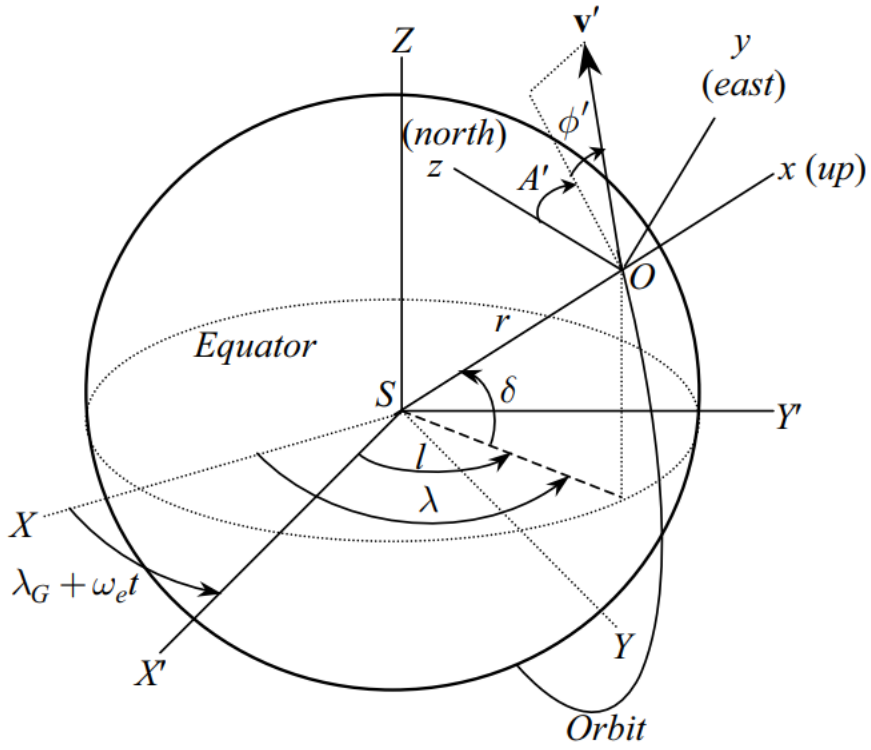
\includegraphics[width=3in]{figuras/PLANETAZUM.png}
        \caption{Referencial girante fixo ao planeta e horizonte local}
        \footnotesize Fonte: \cite{livro:andre}
        \label{fig:PLANETAZUM}
\end{figure} 

Se o planeta possuir velocidade de rotação constante $\omega_{e}$, no mesmo horário do dia cada meridiano irá se alinhar com a direção de uma certa estrela, identificada por uma longitude celeste $\lambda$. É possível realizar a conversão da longitude $l$ para a longitude celeste $\lambda$ conhecendo a longitude celeste do meridiano primário em um dado tempo de referência a partir da equação $\lambda = \lambda_{G} + \omega_{e}t+l$, sendo que a transformação de coordenadas do referencial celeste para o fixo ao planeta é dada por uma rotação elementar em torno do eixo $Z \equiv Z'$ por um ângulo $\lambda-l$. Além disso, é necessário também conhecer a velocidade inercial e relativa. A velocidade relativa depende da velocidade de rotação do planeta e também da posição dada pela distância radial e latitude. A velocidade na órbita relativa ao referencial girante $\textbf{v'}$ possui como coordenadas polares a magnitude da velocidade relativa $v'$, o azimute da velocidade relativa $A'$ e o ângulo de trajetória relativo $\phi '$. As equações necessárias para definir esses valores são dadas pelas equações \ref{eq:1111}, \ref{eq:1112} e \ref{eq:1113}, nesta ordem, sendo em função de $A, \phi, v, \omega_{e}, r$ e $\delta$.

\begin{equation}
    tanA' = tanA-\frac{r\omega_{e} cos\delta}{vcos\phi cosA}
    \label{eq:1111}
\end{equation}

\begin{equation}
    tan\phi '= tan\phi \frac{cosA'}{cosA}
    \label{eq:1112}
\end{equation}

\begin{equation}
    v' = v\frac{sin\phi}{sin\phi '}
    \label{eq:1113}
\end{equation}

\subsection{Elementos orbitais no plano orbital}

No caso de determinação de órbita para um problema de dois corpos a partir de uma única observação de posição e velocidade, a quantidade de elementos orbitais é 6, sendo 3 parâmetros representantes da progressão da órbita no plano orbital e 3 parâmetros representantes da orientação da órbita em respeito a um referencial celeste. Ou seja, a partir da posição inicial e velocidade inicial, medidos no referencial celeste, é necessário determinar $e, a, \tau,\Omega, i$ e $\omega$.

A excentricidade é dada pelo módulo do vetor excentricidade, como mostrado na equação \ref{eq:EXCENTRICIDADEEEEE}, e o semieixo maior é dado pela equação \ref{eq:AAAAA}, já mostrada anteriormente.

\begin{equation}
    e = \left|\left| \textbf{e} \right|\right|
    \label{eq:EXCENTRICIDADEEEEE}
\end{equation}

\begin{equation}
    a = \frac{p}{1-e^{2}}
    \label{eq:AAAAA}
\end{equation}
O tempo de periastro $\tau$ depende do tipo de trajetória, porém é preciso primeiro calcular a anomalia verdadeira $\theta_{0}$ no ponto da órbita observado, o que é realizado a partir das equações \ref{eq:82} (em ambas para evitar ambiguidade).

\begin{equation}
    sin \theta_{0} = \frac{\textbf{r0} \cdot \textbf{p}}{r_{0}p}, \ \ cos \theta_{0} = \frac{p-r_{0}}{er_{0}}
    \label{eq:82}
\end{equation}

Para analisar a equação \ref{eq:82}, é necessário definir $\textbf{p}$, que é dado pela equação \ref{eq:83}, assim, é possível definir a anomalia verdadeira e seguir para a determinação do tempo de periastro $\tau$.

\begin{equation}
\textbf{p} = p\frac{\textbf{h} \times e} {he}
    \label{eq:83}
\end{equation}

\subsection{Órbita elíptica}
Para a órbita elíptica, o tempo de periastro é dado pela equação \ref{eq:84}, onde $t_{0}$ é o tempo de observação medido em algum padrão de referência de tempo, $E_{0}$ é a anomalia excêntrica no ponto observado e $n$ é o movimento médio da órbita elíptica. A anomalia excêntrica é dada pela equação \ref{eq:71} e o movimento médio é dado pela equação \ref{eq:65}.

\begin{equation}
    \tau = t_{0}-\frac{E_{0} - esinE_{0}}{n}
    \label{eq:84}
\end{equation}

\subsection{Órbita parabólica}

Para a órbita parabólica, o tempo de periastro é dado pela equação \ref{eq:85}, obtida através da equação de Barker (\ref{eq:77}).

\begin{equation}
    \tau = t_{0} - \frac {\frac{1}{2} tan \frac{\theta}{2}+\frac{1}{6}tan^{3}\frac{\theta}{2}}  {\sqrt{\frac{\mu}{p^{3}}}}
    \label{eq:85}
\end{equation}

\subsection{Órbita hiperbólica}

O tempo de periastro para a órbita hiperbólica é dada pela equação de Kepler hiperbólica (\ref{eq:74}), a partir da qual se obtém a equação \ref{eq:86}.

\begin{equation}
    \tau = t_{0}-\frac{esinh H_{0}-H_{0} }{(e^{2} - 1)^{3/2} \sqrt{\frac{\mu}{p^{3}}}}
    \label{eq:86}
\end{equation}

\subsection{Parâmetros de orientação da órbita com respeito ao referencial Celeste}

Para determinar $\Omega$, é necessário definir o vetor \textbf{n}, que é dado pela equação \ref{eq:87}, onde \textbf{n} é escrito no referencial celeste. A rotação elementar em torno do eixo $Z$ segundo o ângulo $\Omega$ orienta $n$ com respeito aos vetores diretores \textbf{I} e \textbf{J} do referencial celeste, assim, é tido que o vetor $n$ aponta na direção do eixo $X'$ do sistema intermediário gerado pela rotação elementar. Realizando os cálculos de matrizes, é encontrada a equação \ref{eq:87}, que serve para determinar $\Omega$ sem ambiguidade de quadrante.

\begin{equation}
\left[\begin{array}{l}
n_{X} \\
n_{Y}  \\
n_{Z} 
\end{array}\right] = 
\left[\begin{array}{l}
cos\Omega \\
sin\Omega \\
\  \ \ 0
\end{array}\right] , \ tan \ \Omega = \frac{n_{Y}}{n_{X}}
\label{eq:87}
\end{equation}

Para determinar a inclinação $i$, é realizada a transformação do vetor \textbf{h} do segundo intermediário para o celeste utilizando a matriz de rotação do segundo intermediário para o celeste. Assim, realizando os cálculos, são definidas as equações \ref{eq:88}, porém, é necessário desenvolver duas relações, uma envolvendo seno e outra cosseno, para avaliar o argumento de periastro $\oemga$ sem ambiguidade.

\begin{equation}
 \left[\begin{array}{l}
h_{X} \\
h_{Y}  \\
h_{Z} 
\end{array}\right] = 
\left[\begin{array}{l}
hsin\Omega sin i \\
-hcos\Omega sin i \\
h cos i
\end{array}\right], \ tan \ i = \frac{h_{X}/sin\Omega}{h_{Z}}, \ tan \ i = \frac{-h_{Y}/cos\Omega}{h_{Z}}
\label{eq:88}
\end{equation}

Assim, encontrar o argumento do periastro $\omega$, são definidas as equações \ref{eq:89} (sendo \textbf{ie} um vetor diretor associado ao vetor \textbf{e}, $\textbf{ie} = \textbf{e}/e$, e de forma similar, $\textbf{ih} = \textbf{h}/h$), com as quais se obtém a equação \ref{eq:90}, que possibilita o cálculo sem ambiguidade.

\begin{equation}
    cos \ \omega = \textbf{ie}  \cdot \textbf{n}, \ sin \ \omega = \textbf{ih} \cdot (\textbf{n} \times \textbf{ie})
    \label{eq:89}
\end{equation}

\begin{equation}
    tan \ \omega = \frac{\textbf{ih} \cdot (\textbf{n} \times \textbf{ie})}{\textbf{ie} \cdot \textbf{n}}
    \label{eq:90}
\end{equation}

\section{Manobras Orbitais}
\subsection{Manobras Mono Impulsivas}

\section{Manobras Orbitais com Impulso Único}
Frequentemente, é necessário alterar a trajetória de uma espaçonave usando manobras propulsivas. Considerando que a duração do impulso do foguete aplicado em tal manobra é negligenciável em comparação com o período orbital, é razoável supor que a mudança de velocidade ocorra instantaneamente no ponto de aplicação do impulso. Assim, as manobras orbitais são geralmente consideradas impulsivas.

A manobra impulsiva mais simples ocorre quando as trajetórias inicial e final se intersectam, onde um único impulso de velocidade, $\Delta v$, é suficiente para produzir uma mudança de velocidade de $v_i$ para $v_f$ numa dada posição orbital, $r$. O vetor $v_f$ faz um ângulo $\alpha$ com $v_i$. A relação entre as magnitudes $v_i$, $v_f$ e $\Delta v$ é dada pela equação:
\begin{equation}
\Delta v=\sqrt{{v_i}^2+{v_f}^2-2v_iv_f\cos\alpha}
\label{eq:5.37}
\end{equation}

Uma manobra de impulso único geral pode alterar tanto a forma quanto o plano da órbita. Às vezes, é necessário alterar apenas a forma orbital sem afetar o plano orbital. Essas manobras são ditas coplanares. Numa manobra coplanar, pode haver uma mudança simultânea na velocidade ($v_f -v_i$) e no ângulo de trajetória de voo, $\alpha$, levando a uma nova trajetória coplanar.

Outras vezes é necessário mudar o plano da órbita sem mudar a sua forma. Essa manobra é chamada de manobra de mudança de plano e não envolve modificação da velocidade ou do ângulo da trajetória de voo no ponto do impulso. Para uma mudança de plano por um ângulo $\alpha$ a uma velocidade constante, $v_i$, o seguinte impulso, aplicado em um ângulo $\beta = \alpha/2 + 90^\circ$ para $v_i$, é requerido:
\begin{equation}
\Delta v=2v_i\sin\frac{\alpha}{2}
\label{eq:5.38}
\end{equation}

É evidente pela equação acima que a magnitude do impulso de velocidade para uma mudança de plano por um determinado ângulo é diretamente proporcional à velocidade na qual a mudança é realizada. Portanto, uma mudança de plano por um ângulo pequeno pode exigir um grande impulso de velocidade, o que resulta em um aumento considerável na massa de propelente necessária (causando uma redução na carga útil). Por essa razão, mudanças de plano devem ser realizadas na menor velocidade possível (por exemplo, no apogeu de uma órbita elíptica). Para uma mudança de plano de 60°, a magnitude do impulso é igual à velocidade de voo.

Quando os planos orbitais inicial e final são definidos de forma inequívoca pelos conjuntos dados de $\Omega$, $\omega$, $i$, não podemos escolher o ponto de mudança de plano de forma arbitrária. Para a mudança de plano geral, devemos esperar até que a espaçonave alcance a linha dos nodos formada pela intersecção dos dois planos orbitais, momento em que um impulso de velocidade é aplicado para mudar o plano orbital. Obviamente, se a manobra deve ser realizada por um único impulso de velocidade, as duas órbitas também devem se intersectar na linha dos nodos, o que é verdade apenas para órbitas circulares de raios iguais.

\begin{figure}[h]
        \centering
        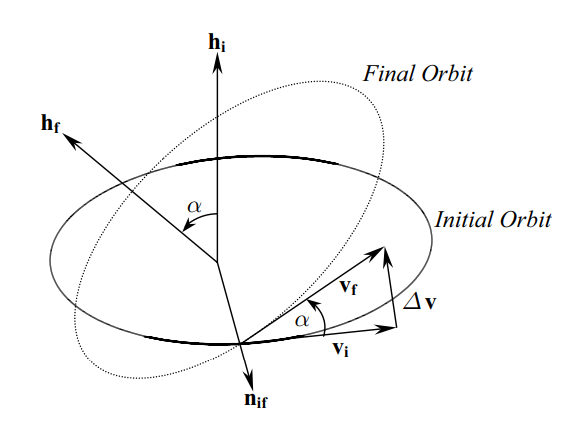
\includegraphics[width=3in]{figuras/monoimspul.png}
        \caption{Manobra Impulsiva generalizada}
        \footnotesize Fonte: \cite{livro:andre}
        \label{fig:monoluiz}
\end{figure} 


A Figura (\ref{fig:monoluiz}) descreve a geometria da mudança de plano geral em termos dos momentos angulares orbital inicial e final, $\mathbf{h_i}$ e $\mathbf{h_f}$, respectivamente. O vetor nodal entre os dois planos indicando o ponto de aplicação do impulso de velocidade é dado por:
\begin{equation}
\mathbf{n}_{\text{if}}=\frac{\mathbf{n}_{\text{i}}\times\mathbf{n}_{\text{f}}}{|\mathbf{h}_{\text{i}}\times\mathbf{h}_{\text{f}}|}
\label{eq:5.39}
\end{equation}

A manobra impulsiva é realizada em $\mathbf{r_i }= r_{i}{\mathbf{n_{if}}}$, a partir do qual a velocidade da mudança de plano, $v_i$, é calculada. O cosseno do ângulo, $\alpha$, entre os dois planos é obtido da seguinte maneira:
\begin{equation}
\cos\alpha=\frac{\textbf{h}_\textbf{i}\cdot\textbf{h}_\textbf{f}}{h_ih_f}
\label{eq:5.40}
\end{equation}

A direção do impulso de mudança de plano em relação ao vetor de velocidade inicial é dada por $\beta = \alpha/2 + 90^\degree$, o que resulta na seguinte expressão para o impulso de velocidade:
\begin{equation}
\Delta\mathbf{v}=\Delta v(\cos\beta\frac{\mathbf{v_i}}{v_i}+\sin\beta\frac{\mathbf{h_i}}{h_i})
\label{eq:5.41}
\end{equation}

levando a

\begin{equation}
\mathbf{v_f}=\mathbf{v_i}+\Delta\mathbf{v}=\mathbf{v_i}+\Delta v(\cos\beta\frac{\mathbf{v_i}}{v_i}+\sin\beta\frac{\mathbf{h_i}}{h_i})
\label{eq:5.42}
\end{equation}

Está claro pelas equações (\ref{eq:5.38}) e (\ref{eq:5.42}) que, para realizar uma mudança de plano sem afetar a velocidade (ou seja, $v_f = v_i$), o ângulo $\beta$ deve ser maior que 90$^\degree$.

\subsection{Manobras Multi Impulsivas}

\par Em manobras mono impulsivas, as órbitas inicial e final se interceptam no ponto de aplicação do impulso. No entanto, para obter órbitas que não se interceptam, pode-se aplicar manobras multi impulsivas ou transferências de baixo empuxo. Transferências de baixo empuxo são especialmente importantes para missões de pequenos satélites, onde um propulsor de baixa tração é acionado continuamente por um longo período de tempo.

\par Manobras multi impulsivas são abordadas neste curso. A Figura (\ref{fig:diagramavelo}) apresenta o diagrama de velocidades em uma manobra multi impulsiva. A maior magnitude da velocidade final $v_f$ é obtida para $\alpha = 0$, enquanto a menor magnitude ocorre para $\alpha = \pi$ rad. Quando o vetor impulso de velocidade $\Delta v$ é colinear com a velocidade inicial, a mudança na magnitude da velocidade é máxima ou mínima, resultando no máximo levantamento ou abaixamento da órbita para a mesma quantidade de propelente.

\begin{figure}[h]
        \centering
        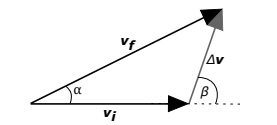
\includegraphics[width=2in]{figuras/diagramaveloci.png}
        \caption{Diagrama de velocidades em uma manobra impulsiva.}
        \footnotesize Fonte: \cite{livro:andre}
        \label{fig:diagramavelo}
\end{figure} 

\par Manobras impulsivas ótimas são realizadas aplicando múltiplos impulsos colineares à velocidade em diferentes pontos da órbita. Em órbitas elípticas, os pontos de aplicação geralmente são periastro ou apoastro. Manobras multi impulsivas referem-se a manobras com múltiplos impulsos colineares ao vetor velocidade e são usadas para alterar a geometria da órbita, mas não sua inclinação.

\par As órbitas inicial e final podem se interceptar ou não, dependendo da técnica adotada. Em manobras multi impulsivas, o conceito de elipse de transferência é importante, que é uma órbita intermediária seguida entre a aplicação de dois impulsos. A técnica de manobra com dois impulsos é chamada de bi-impulsiva.

\subsubsection{ Manobra bi Impulsiva e Elipse de Transferência}

\par Manobras ótimas de transferência entre órbitas elípticas coplanares (com órbitas circulares como casos particulares) são feitas aplicando impulsos tangenciais à trajetória, ou seja, colineares com a velocidade. Em órbitas circulares, qualquer ponto pode ser escolhido, enquanto em órbitas elípticas, os impulsos devem ser aplicados no periastro ou apoastro.

\par Como pode ser visto na Figura (\ref{fig:transbi}) O processo de manobra orbital bi-impulsiva envolve:

\begin{enumerate}
    \item Aplicar o primeiro impulso em qualquer ponto da órbita circular;
    \item O primeiro impulso altera a órbita, gerando uma órbita de transferência elíptica;
    \item O segundo impulso é aplicado no apogeu ou perigeu da órbita de transferência, que coincidirá com o apogeu ou perigeu da órbita final desejada.
\end{enumerate}

\par Há duas opções de órbita de transferência:

\begin{enumerate}
    \item Apogeu da órbita de transferência coincide com o apogeu da órbita final;
    \item Perigeu da órbita de transferência coincide com o perigeu da órbita final.
\end{enumerate}

\begin{figure}[H]
        \centering
        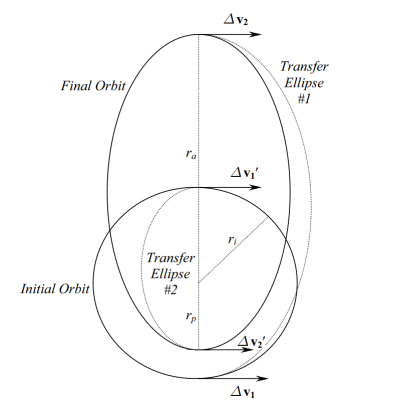
\includegraphics[width=2in]{figuras/transbi.png}
        \caption{Transferência bi impulsiva entre órbitas elípticas.}
        \footnotesize Fonte: \cite{livro:andre}
        \label{fig:transbi}
\end{figure} 

\subsection{Transferência de Hohmann}

\par Quando as órbitas inicial e final são circulares, a manobra ótima bi-impulsiva é chamada de transferência de Hohmann. A transferência de Hohmann consiste na aplicação de dois impulsos tangentes. No levantamento de órbita circular por transferência de Hohmann, ambos os impulsos são aplicados na direção progressiva da órbita.

\begin{figure}[H]
        \centering
        \includegraphics[width=2in]{figuras/homan.png}
        \caption{Transferência de Hohman.}
        Fonte: \ref{}
        \label{fig:homan}
\end{figure} 

\par As distâncias de periastro e apoastro da órbita de transferência são os raios das órbitas inicial e final, respectivamente:

\begin{equation}
r_{p_H}=r_i
\end{equation}

\begin{equation}
r_{a_H}=r_f
\end{equation}

\par O semi eixo maior da órbita de transferência é:

\begin{equation}
a_H=\frac{r_i+r_f}{2}
\end{equation}

\par A magnitude dos dois impulsos de velocidade é:

\begin{equation}
\begin{gathered}
\Delta v_1=v_{p_H}-v_i=\sqrt{\frac{2 \mu}{r_i}-\frac{\mu}{a_H}}-\frac{\mu}{r_i}=\sqrt{\frac{2 \mu}{r_i}-\frac{2 \mu}{r_i+r_f}}-\sqrt{\frac{\mu}{r_i}} \\
\Delta v_1=\sqrt{\frac{2 \mu\left(r_i+r_f\right)-2 \mu r_i}{r_i\left(r_i+r_f\right)}}-\sqrt{\frac{\mu}{r_i}}=\sqrt{\frac{2 \mu r_f}{r_i\left(r_i+r_f\right)}}-\sqrt{\frac{\mu}{r_i}} \\
\Delta v_1=\sqrt{\frac{\mu}{r_i}}\left(\sqrt{\frac{2 r_f}{r_i+r_f}}-1\right)
\label{eq:delta1}
\end{gathered}
\end{equation}


\begin{equation}
\begin{gathered}
\Delta v_2=v_f-v_{a_H}=\sqrt{\frac{\mu}{r_f}}-\sqrt{\frac{2 \mu}{r_f}-\frac{\mu}{a_H}}=\sqrt{\frac{\mu}{r_f}}-\sqrt{\frac{2 \mu}{r_f}-\frac{2 \mu}{r_i+r_f}} \\
\Delta v_2=\sqrt{\frac{\mu}{r_f}}-\sqrt{\frac{2 \mu\left(r_i+r_f\right)-2 \mu r_f}{r_f\left(r_i+r_f\right)}}=\sqrt{\frac{\mu}{r_f}}-\sqrt{\frac{2 \mu r_i}{r_f\left(r_i+r_f\right)}} \\
\Delta v_2=\sqrt{\frac{\mu}{r_f}}\left(1-\sqrt{\frac{2 r_i}{r_i+r_f}}\right)
\label{eq:delta2}
\end{gathered}
\end{equation}


Se o processo de transferência for de uma órbita de maior raio (mais alta) para uma de menor (mais baixa), a equação do impulso de velocidade é:

\begin{equation}
\Delta v_1=v_{a_H}-v_i=\sqrt{\frac{2 \mu}{r_i}-\frac{\mu}{a_H}}-\frac{\mu}{r_i}=\sqrt{\frac{\mu}{r_i}}\left(\sqrt{\frac{2 r_f}{r_i+r_f}}-1\right)
\label{eq:delta1fin}
\end{equation}

\begin{equation}
\Delta v_2=v_f-v_{p_H}=\sqrt{\frac{\mu}{r_f}}-\sqrt{\frac{2 \mu}{r_f}-\frac{\mu}{a_H}}=\sqrt{\frac{\mu}{r_f}}\left(1-\sqrt{\frac{2 r_i}{r_i+r_f}}\right)
\label{eq:delta2fin}
\end{equation}

\par No abaixamento de órbita circular por transferência de Hohmann, ambos os impulsos são aplicados na direção oposta à órbita, pois $r_i>r_f$. Nesse caso, ambos os impulsos de velocidade são negativos. 

\par A órbita de transferência dura meio período, que é o tempo da transferência de Hohmann. Este tempo pode ser calculado pela seguinte equação, tendo como base a equação \ref{eq:62} dependendo apenas do semi eixo maior da órbita de transferência:

\begin{equation}
T_h=\pi\sqrt{\frac{a_H^3}{\mu}},\text{ou} \, T_h=\pi\sqrt{\frac{(r_i+r_f)^3}{8\mu}}
\end{equation}


%%%%%%%%%%%%% AULA 11 %%%%%%%%%%%%%%%%%%%%%%%%%%%

\section{Órbitas Perturbadas}
\subsection{Aceleração Perturbativa}
\par A aceleração perturbativa ocorre quando o movimento no problema dos dois corpos ideal é afetado por forças além da atração gravitacional mútua. No problema dos dois corpos ideal, consideramos apenas órbitas Keplerianas (elipse, hipérbole e parábola) com coeficientes constantes no plano orbital. Entretanto, na realidade, há sempre perturbações extras.

\par Perturbações podem ser conservativas ou não conservativas. Exemplos de perturbações conservativas incluem:

\begin{itemize}
  \item Gravidade de terceiro corpo;
  \item Achatamento de um planeta, alterando sua geometria de uma esfera;
  \item Força magnética proveniente da interação de correntes elétricas internas do corpo com o campo magnético do planeta.
\end{itemize}

\par Exemplos de perturbações não conservativas são:

\begin{itemize}
  \item Arrasto atmosférico;
  \item Pressão solar;
  \item Disparo de propulsor.
\end{itemize}

\par Resolver um problema com várias forças perturbativas agindo simultaneamente é desafiador. No entanto, muitas situações práticas apresentam perturbações que não se manifestam com a mesma intensidade, na mesma região e ao mesmo tempo. Isso permite analisar o efeito da perturbação principal, ignorando as demais.

\par Por exemplo:

\begin{itemize}
  \item Em órbita baixa, a perturbação de maior intensidade costuma ser o arrasto atmosférico;
  \item Em uma órbita interplanetária, a perturbação mais relevante costuma ser a de terceiro corpo.
\end{itemize}

\par Em termos matemáticos, conforme visto na aula 3, o problema dos dois corpos é formulado para o movimento relativo de uma partícula de massa $m$ em relação a outra de massa $M$. A equação do movimento é dada por:

\begin{equation}
\frac{d^2\mathbf{r}}{dt^2}+\mu\frac{\mathbf{r}}{r^3}=0 \quad 
\label{eq:1L}
\end{equation}

\par Onde $\mathbf{r}$ é o vetor posição relativa da partícula $m$ com respeito a $M$, e $\mu = GM$ quando $m \ll M$. Alternativamente, podemos considerar que $M$ é um planeta esférico e $m$ um corpo de dimensões insignificantes em comparação a ele. Nesse caso, o vetor posição é medido entre $m$ e o centro de massa (CM) do planeta, sendo válido, por exemplo, para o movimento de satélites artificiais ao redor da Terra.

\par Nesse contexto, a maneira mais comum de avaliar uma perturbação é inserindo uma aceleração perturbativa $\mathbf{a}_d$ no lado direito da equação 1:

\begin{equation}
\frac{d^2\mathbf{r}}{dt^2}+\mu\frac{\mathbf{r}}{r^3}=\mathbf{a}_d \quad 
\label{eq:2L}
\end{equation}

\par A equação (\ref{eq:2L}) leva em consideração a aceleração perturbativa, permitindo uma análise mais precisa das órbitas em situações reais onde perturbações adicionais, além da atração gravitacional mútua, estão presentes.

\par Quando a força perturbativa é conservativa, a aceleração perturbativa pode ser escrita como o gradiente de uma função potencial $\Phi$:

\begin{equation}
\mathbf{a}_d = \nabla\Phi^T
\label{eq:3L}
\end{equation}

\par Neste caso, ao invés de um problema vetorial de 3 componentes, o problema é descrito por uma função escalar $\Phi$, que representa o potencial perturbativo.

\par A aceleração perturbativa (ou potencial perturbativo) é estudada em casos específicos. O primeiro deles é o efeito do achatamento dos polos do planeta. Este efeito leva em consideração que a forma do planeta não é perfeitamente esférica, mas sim, um pouco achatada nos polos. Essa deformação na forma do planeta resulta em perturbações no movimento orbital de satélites e outros corpos celestes próximos.

\subsection{Efeito do Achatamento dos Pólos}

\par Como discutido anteriormente, a equação de dinâmica do problema de dois corpos é válida quando o planeta possui massa esfericamente distribuída, de modo que seu modelo gravitacional é o mesmo de uma massa pontual:

\begin{equation}
g = GM \frac{\mathbf{r}}{r^3}
\label{eq:4L}
\end{equation}

\par Se um planeta possui achatamento nos polos, seu modelo gravitacional é determinado por uma expansão em série do potencial gravitacional. Quando o corpo possui massa distribuída de maneira axis simétrica, o potencial é determinado pelas constantes de Love (denominadas $J_n$). 

\par Neste contexto, a dinâmica de órbita perturbada da equação 2 é utilizada, com a aceleração perturbativa dada pela equação (\ref{eq:3L}):

\begin{equation}
\frac{d^2\mathbf{r}}{dt^2} + \mu \frac{\mathbf{r}}{r^3} = \nabla\Phi^T
\label{eq:5L}
\end{equation}

\par Na aula 2, foi determinado o potencial gravitacional de um corpo axis simétrico:

\begin{equation}
\Phi = \frac{\mu}{r} - \frac{\mu}{r} \sum_{n=2}^{\infty} \left(\frac{R_e}{r}\right)^n J_n P_n(\sin\delta)
\label{eq:6L}
\end{equation}

\par Onde: $R_e$ é o raio equatorial do planeta, $\delta$ é a latitude, $P_n$ é o polinômio de Legendre de grau n, $J_n$ é a n-ésima constante de Love. Na equação (\ref{eq:6L}), o primeiro termo da soma $(\mu/r)$ é o potencial gravitacional da massa pontual (igual ao de um planeta com massa esfericamente distribuída). Os demais estão relacionados com a não esfericidade do planeta. Sendo assim, o potencial perturbativo é:

\begin{equation}
\Phi = -\frac{\mu}{r} \sum_{n=2}^{\infty} \left(\frac{R_e}{r}\right)^n J_n P_n(\sin\delta)
\label{eq:7L}
\end{equation}

\par Assim, o efeito do achatamento dos polos é avaliado determinando-se a solução da equação diferencial abaixo:

\begin{equation}
\frac{d^2\mathbf{r}}{dt^2} + \mu \frac{\mathbf{r}}{r^3} = -\frac{\partial}{\partial\mathbf{r}} \frac{\mu}{r} \sum\limits_{n=2}^{\infty} \left(\frac{R_e}{r}\right)^n J_n P_n(\sin\delta)
\label{eq:8L}
\end{equation}

\subsubsection{Equações Planetárias de Lagrange}

\par As Equações Planetárias de Lagrange fornecem uma maneira de encontrar a solução perturbada devido a um potencial perturbativo. Supomos que a solução perturbada seja uma função dos 6 parâmetros das órbitas keplerianas e do tempo, agrupados em um vetor $\mathbf{c}$:

\begin{equation}
\mathbf{c}=[c_1,c_2,c_3,c_4,c_5,c_6]^T=[a,e,\tau,\Omega,i,\omega]^T
\label{eq:9L}
\end{equation}

\par As funções genéricas $f$ e $g$ são usadas para representar a solução:

\begin{equation}
r = f(\mathbf{c}, t), \quad v = g(\mathbf{c}, t)
\label{eq:10L}
\end{equation}

\par E temos:

\begin{equation}
\mathbf{v}=\frac{d\mathbf{r}}{dt}=\frac{\partial\mathbf{f}}{\partial t}
\label{eq:11L}
\end{equation}

\par Quando $f$ e $g$ são soluções para o problema não perturbado, os parâmetros orbitais são constantes. O método de solução consiste em substituir na equação da aceleração perturbativa a solução da equação não perturbada. E aplicando  regra da cadeira temos que:

\begin{equation}
\frac{\partial\mathbf{f}}{\partial\mathbf{c}}\frac{d\mathbf{c}}{dt}=0
\label{eq:12L}
\end{equation}

e

\begin{equation}
\frac{d^2\mathbf r}{dt^2}=\frac{\partial^2\mathbf f}{\partial t^2}+\frac{\partial\mathbf g}{\partial\mathbf c}\frac{d\mathbf c}{dt}  
\label{eq:13L}
\end{equation}

\par As equações indicam que a derivada dos parâmetros orbitais $\frac{d\mathbf{c}}{dt}$ é ortogonal à matriz jacobiana $\frac{\partial\mathbf{f}}{\partial\mathbf{c}}$. Essa relação é útil para analisar a dinâmica de órbitas perturbadas e entender como as perturbações afetam os parâmetros orbitais.E substituindo as equações (\ref{eq:10L}) e (\ref{eq:13L}) na equação (\ref{eq:5L}) e assumindo que $f$ e $g$ satisfazem a equação dinâmica do problema não perturbado, temos que a equação diferencial perturbativo como: 

\begin{equation}
{\frac{\partial\mathbf{g}}{\partial\mathbf{c}}}{\frac{d\mathbf{c}}{d t}}=\nabla\Phi^{T}
\label{eq:14L}
\end{equation}

\par As equações (\ref{eq:12L}) e (\ref{eq:14L})  formam um conjunto de 6 equações diferenciais para determinar a variação dos parâmetros orbitais em função da aceleração perturbativa:

\begin{equation}
 \frac{\partial\mathbf f}{\partial\mathbf c}\frac{d\mathbf c}{dt}=0
 \label{eq:15L}
\end{equation}
\begin{equation}
 \frac{\partial\mathbf{g}}{\partial\mathbf{c}}\frac{d\mathbf{c}}{dt}=\nabla\Phi^T   
 \label{eq:16L}
\end{equation}

\par Para continuar com a dedução, temos as seguintes definições de notação:
\begin{itemize}
    \item $\hat{\mathbf{r}} = \mathbf{f}$ e $\hat{\mathbf{v}} = \mathbf{g}$ são as soluções do problema não perturbado (kepleriano);
    \item $\tilde{\mathbf{r}}$ e $\tilde{\mathbf{v}}$ são as perturbações das soluções keplerianas, de modo que:
    \item Soluções perturbadas: $\mathbf{r} = \hat{\mathbf{r}} + \tilde{\mathbf{r}}$ e $\mathbf{v} = \hat{\mathbf{v}} + \tilde{\mathbf{v}}$.
\end{itemize}

\par Após reescrever as equações e usar álgebra matricial, obtemos:

\begin{equation}
\left[\begin{array}{c}\frac{\partial\hat{\textbf{r}}}{\partial\textbf{c}}\\ \frac{\partial\hat{\textbf{v}}}{\partial\textbf{c}}\end{array}\right]\frac{d\textbf{c}}{dt}=\left[\begin{array}{c}\textbf{0}_{3\times1}\\ \nabla\Phi^T\end{array}\right]
\label{eq:16L}
\end{equation}

\par Multiplicamos ambos os lados pela matriz:

\begin{equation}
\mathbf{M}=\left[-\left(\frac{\partial\hat{\mathbf{v}}}{\partial\mathbf{c}}\right)^T\left(\frac{\partial\hat{\mathbf{r}}}{\partial\mathbf{c}}\right)^T\right]
\label{eq:20L}
\end{equation}

\par Resultando em:

\begin{equation}
\left(\left(\frac{\partial\hat{\mathbf{r}}}{\partial\mathbf{c}}\right)^T\frac{\partial\hat{\mathbf{v}}}{\partial\mathbf{c}}-\left(\frac{\partial\hat{\mathbf{v}}}{\partial\mathbf{c}}\right)^T\frac{\partial\hat{\mathbf{r}}}{\partial\mathbf{c}}\right)\frac{d\mathbf{c}}{d t}=\left(\frac{\partial\hat{\mathbf{r}}}{\partial\mathbf{c}}\right)^T\nabla\Phi^T
\label{eq:21L}
\end{equation}

\par Por derivações e manipulações matemáticas é possível chegar na matriz de Lagrange, dada por:

\begin{equation}
\mathbf{L}=\left(\frac{\partial \hat{\mathbf{r}}}{\partial \mathbf{c}}\right)^T \frac{\partial \hat{\mathbf{v}}}{\partial \mathbf{c}}-\left(\frac{\partial \hat{\mathbf{v}}}{\partial \mathbf{c}}\right)^T \frac{\partial \hat{\mathbf{r}}}{\partial \mathbf{c}}
\label{eq:25L}
\end{equation}

\begin{equation}
\mathbf{L} \frac{d \mathbf{c}}{d t}=\frac{\partial \Phi^T}{\partial \mathbf{c}}
\label{eq:26L}
\end{equation}

\par Que por sua vez é antissimétrica e não depende explicitamente do tempo. A equação (\ref{eq:26L}) define 6 equações diferenciais de primeira ordem, uma para cada parâmetro orbital. Elas são equações diferenciais de primeira ordem que determinam a taxa de variação dos parâmetros orbitais em função do potencial perturbativo. Estas equações diferenciais são chamadas de equações planetárias de Lagrange.

\subsection{Variações dos Elementos Orbitais com Achatamento dos Pólos}

\par A seguir, são apresentadas as equações planetárias de Lagrange para o caso estudado:

\begin{itemize}
    \item Os parâmetros orbitais são os clássicos: $\mathbf{c} = [a, e, \tau, \Omega, i, \omega]^T$;
    \item O potencial perturbativo está associado ao planeta com achatamento nos pólos;
    \item Ou seja, o potencial perturbativo é dado pela equação 7, sendo função das constantes de Jefiery.
\end{itemize}

\par As equações diferenciais que apresentam a taxa de variação dos elementos orbitais serão apresentadas sem demonstração.
As taxas de variação de $\Omega$ e $\omega$, levando em conta a primeira constante de Jefiery ($J_2$), são:

\begin{equation}
\dot\Omega = \frac{h}{\mu}\frac{\sin(\omega+\theta)}{\sin i(1+e\cos\theta)}\left(-\frac{3\mu}{2r^2}J_2\left(\frac{R_e}{r}\right)^2\sin2i\sin(\omega+\theta)\right)
\label{eq:27L}
\end{equation}

\begin{equation}
-\frac{r\sin(\omega+\theta)}{h\tan i}\left(-\frac{3\mu}{2r^2}J_2\left(\frac{R_e}{r}\right)^2\sin2i\sin(\omega+\theta)\right)
\label{eq:28L}
\end{equation}

\par Entretanto, os efeitos instantâneos não são significativos, eles geram pouco impacto sobre uma única órbita. O maior efeito é cumulativo, ou seja: mudanças perceptíveis ocorrem somente depois de
um número significativo de voltas. Neste sentido, algumas referências costumam escrever as equações diferenciais dos parâmetros orbitais em termos da média relativa a uma órbita completa. Portanto, temos que as derivadas médias dos parâmetros $a,e,\omega$ e $\Omega$ levando em conta somente a primeira constante: 

\begin{equation}
\frac{d\bar{a}}{dt}=0
\end{equation}
\begin{equation}
\frac{d\bar{e}}{dt}=0
\end{equation}
\begin{equation}
\frac{d\bar{\omega}}{dt}=\frac{3}{4}nJ_2\left(\frac{R_e}{p}\right)^2(5\cos^2i-1)
\end{equation}
\begin{equation}
\frac{d\bar{\Omega}}{dt}=\frac{3}{4}nJ_2\left(\frac{R_e}{p}\right)^2\cos i
\end{equation}

\par Dessa forma, o efeito da perturbação devido ao achatamento dos polos, quando apenas a primeira constante de Jefiery (a mais significativa) é levada em consideração, mantém o formato da órbita inalterado. Isso ocorre porque, ao longo de órbitas completas, as variações médias do semieixo maior e da excentricidade são nulas.

\par Por outro lado essa perturbação provoca mudança na direção da órbita: 
\begin{itemize}
    \item A variação da longitude celeste do nodo ascendente está relacionada à mudança de direção linha dos nodos;
    \item A variação do argumento de periastro está associada à mudança de direção da linha dos apsides.
\end{itemize}

\subsection{Órbita Hélio Síncrona}
\par Um efeito benéfico da regressão nodal é a órbita heliossíncrona ilustrada na figura (\ref{fig:sol}), utilizada para mapeamento fotográfico e satélites de observação. Uma órbita heliossíncrona permite uma elevação solar constante em um dado ponto, o que é desejável para fotografias de superfície.

\begin{figure}[h]
        \centering
        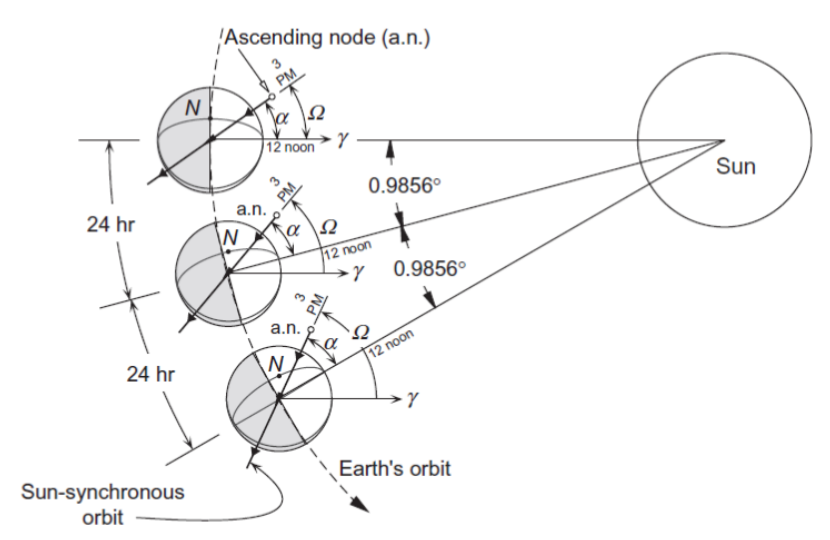
\includegraphics[width=2in]{figuras/sol.png}
        \caption{Órbita hélio síncrona.}
        \footnotesize Fonte: \cite{livro:andre}
        \label{fig:sol}
\end{figure} 

\par Em uma órbita heliossíncrona, o plano orbital forma um ângulo constante com a radial do Sol até a Terra. Para isso, o plano orbital deve girar no espaço inercial com uma velocidade angular igual à da Terra ao redor do Sol, que é 360° a cada 365,26 dias, ou 0,9856° por dia. Este tipo de órbita síncrona cruza uma dada latitude em um tempo solar fixo. Na ilustração da figura (\ref{fig:sol}), isso ocorre às 15h. Durante cada órbita, o satélite vê a mesma área da superfície terrestre no mesmo horário. 

\subsection{Órbita Moliya}
\par Outra aplicação especial desenvolvida com base nos resultados desta aula são as órbitas Molniya, utilizadas pela Rússia para satélites de comunicação em altas latitudes, onde se situa a maior parte do país. Uma órbita Molniya é ilustrada na figura (\ref{fig:mol}).

\begin{figure}[h]
        \centering
        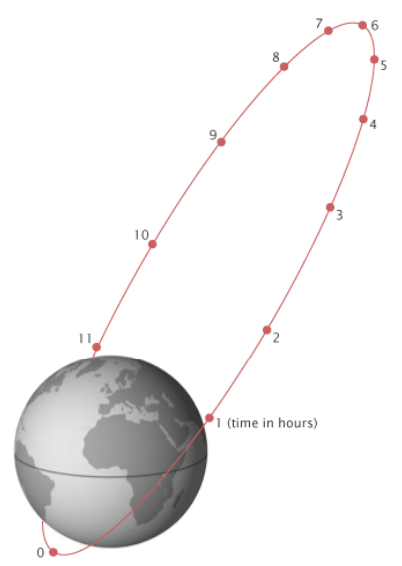
\includegraphics[width=2in]{figuras/mol.png}
        \caption{Órbita Moliya.}
        \footnotesize Fonte: \cite{livro:andre}
        \label{fig:mol}
\end{figure} 

\par Para que as comunicações sejam efetivas, os satélites devem permanecer em altas latitudes por longos períodos. Isso resulta em órbitas altamente elípticas, adotando o valor de excentricidade $e = 0.73$. O período dessas órbitas é aproximadamente 12 horas, com apogeu na direção do polo norte.

\par Para uma órbita Molniya, é crucial que a latitude do periastro não mude devido à rotação dos apsides, provocada pelo achatamento da Terra. Então, uma órbita Molniya sempre tem a inclinação crítica $i_c = 63.44^\circ$, para a qual $\dot{\omega} = 0$.

\par A alta inclinação de uma órbita Molniya é obtida a partir de lançamentos do centro de Plesetsk, localizado em uma latitude de $62.8^\circ$. Lançar de uma latitude próxima da inclinação da órbita otimiza o lançamento, reduzindo o consumo de propelente, o que é especialmente desejável para inclinações altas.

%%%%%%%%%%%%%%%%%%% AULA 12 %%%%%%%%%%%%%%%%%%%%%%%%%%%%%%%%%
\section{Órbitas Perturbadas}
\subsection{Perturbação de 3º corpo}

\par A perturbação gravitacional de um terceiro corpo em uma órbita de dois corpos é modelada de maneira similar à perturbação gravitacional de um corpo primário não esférico. Considere a órbita gerada pela atração gravitacional mútua de dois corpos $m_1$ e $m_2$, perturbados pela presença de um terceiro corpo $m_3$, como visto na figura (\ref{fig:3corpo}). As equações do movimento para os corpos de massa $m_1$ e $m_2$ são:

\begin{equation}
\frac{d^2\mathbf r_1}{dt^2}=-\frac{Gm_2}{r_{21}^3}\left(\mathbf r_1-\mathbf r_2\right)-\frac{Gm_3}{r_{31}^3}\left(\mathbf r_1-\mathbf r_3\right)   
\label{eq:1a12}
\end{equation}
\begin{equation}
\frac{d^2\mathbf r_2}{dt^2}=-\frac{Gm_1}{r_{21}^3}\left(\mathbf r_2-\mathbf r_1\right)-\frac{Gm_3}{r_{32}^3}\left(\mathbf r_2-\mathbf r_3\right)
\label{eq:2a12}
\end{equation}

\begin{figure}[h]
        \centering
        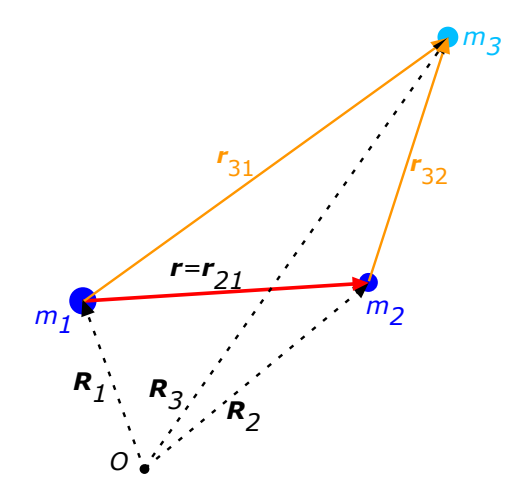
\includegraphics[width=2in]{figuras/3corpo.png}
        \caption{Diagrama da atração gravitacional entre 3 corpos.}
        \footnotesize Fonte: \cite{livro:andre}
        \label{fig:3corpo}
\end{figure} 

\par Subtraindo a equação (\ref{eq:1a12}) da equação (\ref{eq:2a12}), obtemos a equação do movimento relativo:

\begin{equation}
\frac{d^2\mathbf{r}}{dt^2}+\mu\frac{\mathbf{r}}{r^3}=Gm_3\left(\frac{\mathbf{r}_{32}}{r_{32}^3}-\frac{\mathbf{r}_{31}}{r_{31}^3}\right)
\label{eq:3a12}
\end{equation}

onde $\mu = G(m_1 + m_2)$. O lado esquerdo da equação (\ref{eq:3a12}) é o mesmo do problema de dois corpos, enquanto o lado direito é a aceleração perturbativa sobre o sistema de dois corpos. Essa aceleração depende da distância do terceiro corpo até cada um dos primários e da constante gravitacional de $m_3$, $\mu_3 = Gm_3$. Além do mais, o potencial perturbativo do terceiro corpo é dado por:

\begin{equation}
\Phi=Gm_3\left(\frac{1}{r_{32}}-\frac{\mathbf{r}\cdot\mathbf{r}_{31}}{r_{31}^3}\right)
\label{eq:7a12}
\end{equation}

\par A perturbação de terceiro corpo pode ser estudada sem perda de generalidade para a ação de uma quantidade maior de corpos perturbativos. Entretanto, o efeito de terceiro corpo é satisfatório para a maioria das missões espaciais. O potencial perturbativo de terceiro corpo pode ser expandido segundo uma série infinita de polinômios de Legendre:

\begin{equation}
\Phi=\frac{G m_3}{r_{31}}\left[1+\sum_{n=2}^\infty\left(\frac{r}{r_{31}}\right)^n P_n(\cos\gamma)\right]
\label{eq:8a12}
\end{equation}

onde $\gamma$ é o ângulo entre os vetores $\mathbf{r}$ e $\mathbf{r}_{31}$. A equação do movimento perturbado se torna:

\begin{equation}
\frac{d^{2}\mathbf{r}}{d t^{2}}+\frac{\mu\mathbf{r}}{r^{3}}=\frac{G m_{3}}{r_{31}^{2}}\sum_{n=1}^{\infty}\left(\frac{r}{r_{31}}\right)^{n}\left(P_{n+1}^{\prime}(\cos\gamma)\frac{\mathbf{r}_{31}}{r_{31}}-P_{n}^{\prime}(\cos\gamma)\frac{\mathbf{r}}{r}\right)
\label{eq:9a12}
\end{equation}

onde $P_n'$ é a derivada de um polinômio de Legendre com respeito ao seu argumento, determinada pela regra de recorrência:

\begin{equation}
P_n'(\nu)=\nu P_{n-1}'(\nu)+n P_{n-1}(\nu)
\label{eq:10a12}
\end{equation}

\subsection{Esfera de Influência e Aproximação por Seções Cônicas}

\par Diferentemente do problema de dois corpos ideal ou do caso perturbado pela gravidade de um planeta não esférico, o movimento perturbado por terceiro corpo não possui solução analítica. Uma aproximação comumente usada em mecânica orbital está associada ao conceito de esfera de influência. Dentro dessa esfera, a gravidade de um planeta domina, enquanto fora dela a atração gravitacional do Sol é predominante.

\par Assumindo que o corpo m2 esteja sob a influência gravitacional de dois primários, as equações do movimento podem ser expressas como:

\begin{equation}
\frac{d^2\mathbf{r}}{dt^2}+G(m_1+m_2)\frac{\mathbf{r}}{r^3}=Gm_3\left(\frac{\mathbf{r}_{32}}{r_{32}^3}-\frac{\mathbf{r}_{31}}{r_{31}^3}\right)
\label{eq:11a12}
\end{equation}

\begin{equation}
\frac{d^2\mathbf{r}_{23}}{dt^2}+G(m_3+m_2)\frac{\mathbf{r}_{23}}{r_{23}^3}=Gm_1\left(\frac{\mathbf{r}_{31}}{r_{31}^3}-\frac{\mathbf{r}}{r^3}\right)
\label{eq:12a12}
\end{equation}

\par A equação (\ref{eq:11a12}) trata do movimento relativo do corpo m2 com respeito a m1, onde m3 gera a perturbação. Este modelo subentende uma órbita aproximadamente kepleriana de m2 com respeito ao primário m1, sendo m3 o terceiro corpo impondo uma perturbação. Isso pode ser visualizado na figura (\ref{fig:esfera}).

\begin{figure}[h]
        \centering
        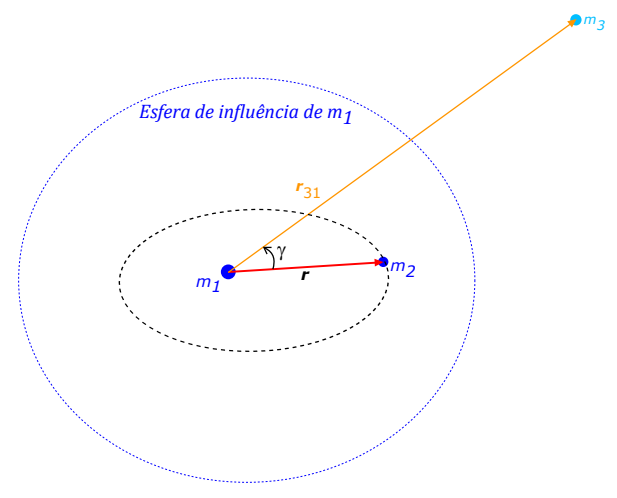
\includegraphics[width=2in]{figuras/esfera.png}
        \caption{ Ilustração da esfera de influência do primário m1.}
        \footnotesize Fonte: \cite{livro:andre}
        \label{fig:esfera}
\end{figure} 

\par Da mesma forma a equação (\ref{eq:12a12}) trata do movimento relativo do corpo m2 em relação a m3. Ela é obtida por analogia à equação (\ref{eq:11a12}), trocando m1 por m3 e vice-versa, $r_{21} = r$ por $r_{23}$, $r_{32}$ por $r_{12} = -r$ e $r_{31}$ por $r_{13} = -r_{31}$. 

\par Na equação (\ref{eq:12a12}), o corpo m3 é o primário e m1 gera a perturbação. Ou seja, este modelo supõe uma órbita aproximadamente kepleriana de m2 em relação a m3, sendo m1 o terceiro corpo gerador da perturbação. A melhor aproximação é dada pela equação que apresenta a menor razão entre a aceleração perturbativa e a aceleração do primário.

Para aprofundar essa questão, serão avaliadas as acelerações perturbativas em comparação com as do primário. 

Na equação (\ref{eq:11a12}), a aceleração do primário é o efeito de m1 sobre m2, enquanto a perturbação é o efeito de m3 sobre m2:

\begin{equation}
\mathbf{a}_{21}=-G(m_1+m_2)\frac{\mathbf{r}}{r^3}
\label{eq:13a12}
\end{equation}

\begin{equation}
\mathbf{a}_{d_{23}}=Gm_3\left(\frac{\mathbf{r}_{32}}{r_{32}^3}-\frac{\mathbf{r}_{31}}{r_{31}^3}\right)
\label{eq:14a12}
\end{equation}

Na equação (\ref{eq:12a12}), a aceleração do primário é o efeito de $m_3$ sobre $m_2$, enquanto a perturbação é o efeito de $m_1$ sobre $m_2$:

\begin{equation}
\mathbf{a}_{23}=-G(m_3+m_2)\frac{\mathbf{r}_{23}}{r_{23}^3}
\label{eq:15a12}
\end{equation}

\begin{equation}
\mathbf{a}_{d_{21}}=G m_1\left(\frac{\mathbf{r}_{31}}{r_{31}^3}-\frac{\mathbf{r}}{r^3}\right)
\label{eq:16a12}
\end{equation}

A precisão da aproximação da órbita kepleriana de $m_2$ com respeito a $m_1$ é medida calculandose a razão entre: a magnitude da perturbação de m3 sobre $m_2$ e a magnitude da aceleração de $m_2$ provocada por $m_1$. Para $\frac{a_{d_{23}}}{a_{21}}$, temos:

\begin{equation}
\frac{a_{d_{23}}}{a_{21}} = \frac{||\mathbf{a}_{d_{23}}||}{||\mathbf{a}_{21}||} 
\label{eq:17a12}
\end{equation}

Para $\frac{a_{d_{23}}}{a_{21}} << 1$ a perturbação provocada pelo corpo $m_3$ é pouco significativa quando comparada à aceleração imposta por $m_1$.


Por outro lado, a aproximação de órbita kepleriana de $m_2$ com respeito a m3 é avaliada pela razão entre: a magnitude da perturbação de $m_1$ sobre $m_2$ e a magnitude da aceleração de m2 provocada por $m_3$. Para $\frac{a_{d_{21}}}{a_{23}}$, temos:

\begin{equation}
\frac{a_{d_{21}}}{a_{23}} = \frac{||\textbf{a}_{d_{21}}||}{||\textbf{a}_{23}||}
\label{eq:18a12}
\end{equation}

Para $\frac{a_{d_{21}}}{a_{23}} << 1$ a perturbação provocada pelo corpo m1 é pouco significativa quando comparada à aceleração imposta por m3.

\par Com esses desenvolvimentos chegamos em dois pontos, a Primeira razão de perturbação, vista na equação (\ref{eq:19a12}), e a Segunda razão de perturbação, vista na equação (\ref{eq:20a12}).

\begin{equation}
\begin{aligned}
\frac{a_{d_{23}}}{a_{21}} & =\frac{m_3}{m_1+m_2}\left(\left(\frac{r}{r_{31}}\right)^4+\left(\left(\frac{r}{r_{31}}\right)^{-2}-2 \cos \gamma\left(\frac{r}{r_{31}}\right)^{-1}+1\right)^{-\frac{3}{2}}\left(\left(\frac{r}{r_{31}}\right)^3-\frac{r}{r_{31}}\right)+\right. \\
& \left.\left(\left(\frac{r}{r_{31}}\right)^{-2}-2 \cos \gamma\left(\frac{r}{r_{31}}\right)^{-1}+1\right)^{-2}-\left(\left(\frac{r}{r_{31}}\right)^{-2}-2 \cos \gamma\left(\frac{r}{r_{31}}\right)^{-1}+1\right)^{-\frac{1}{2}}\left(\frac{r}{r_{31}}\right)^3\right)^{\frac{1}{2}}
\label{eq:19a12}
\end{aligned}
\end{equation}

\begin{equation}
\begin{aligned}
\frac{a_{d_{21}}}{a_{23}} & =\frac{m_1}{m_3+m_2}\left(\left(\left(\frac{r}{r_{31}}\right)^2-2 \cos \gamma \frac{r}{r_{31}}+1\right)^2+\left(\left(\frac{r_{31}}{r}\right)^2-2 \cos \gamma \frac{r_{31}}{r}+1\right)^2+\right. \\
& \left.-2 \cos \gamma\left(\left(\frac{r}{r_{31}}\right)^2-2 \cos \gamma \frac{r}{r_{31}}+1\right)\left(\left(\frac{r_{31}}{r}\right)^2-2 \cos \gamma \frac{r_{31}}{r}+1\right)\right)^{\frac{1}{2}}
\label{eq:20a12}
\end{aligned}
\end{equation}


\subsubsection{Esfera de Influência} 
\par As expressões $\frac{a_{d_{23}}}{a_{21}}$ e $\frac{a_{d_{21}}}{a_{23}}$ são usadas para determinar a
região onde a ação gravitacional de $m1$ predomina sobre a de $m3$, que nada mais é do que a esfera de influência de $m_1$ com respeito a $m_3$. Essa é região dentro da qual a perturbação relativa de $m_3$ é menor que a perturbação de $m_1$:

\begin{equation}
\frac{a_{d_{23}}}{a_{21}}<\frac{a_{d_{21}}}{a_{23}}
\label{eq:23a12}
\end{equation}

\par Pelas equações (\ref{eq:19a12}) e (\ref{eq:20a12}), verifica-se que a esfera de influência depende das massas $m_1, m_2$ e $m_3$, da distância $r_{13}$ entre o primeiro e o terceiro corpo, bem como do ângulo $\gamma$. Rigorosamente falando, devido à dependência com $\gamma$, a distância $r$ sobre a borda da esfera de influência depende da posição orbital de $m_2$ com respeito ao corpo $m_1$.

\subsection{Efeito do arrasto atmosférico}
\par As espaçonaves em órbita baixa experimentam um arrasto atmosférico significativo, cuja magnitude é proporcional ao produto da densidade atmosférica, $\rho$, e o quadrado da velocidade relativa, $\dot{r}^2$. Como o arrasto se opõe ao movimento orbital, podemos expressar a equação de movimento perturbada por: 

\begin{equation}
\frac{\mathrm{d}^2 \mathbf{r}}{\mathrm{d} t^2}+\frac{\mu}{r^3} \mathbf{r}=-q \dot{r} \mathbf{r}
\label{eq:1aula12}
\end{equation}

onde 

\begin{equation}
q \doteq \frac{1}{2} \rho \frac{C_D A}{m_2}
\label{eq:2aula12}
\end{equation}

E $C_D$ é o coeficiente de arrasto com base numa área de referência, $A$. Geralmente, a suposição de fluxo livre-molecular é válida nas altitudes orbitais, que de acordo com os métodos estudados produz um valor de coeficiente de arrasto, $C_D \approx 2$, para a maioria das formas, com base na área máxima de seção transversal voltada para o fluxo. A dependência do arrasto na velocidade, ao invés da posição, torna-o uma força não conservativa, que resulta em um declínio da energia orbital, $\epsilon = - \mu / 2a$, e portanto, do semi-eixo maior, $a$. Tomando o produto escalar da desaceleração devido ao arrasto com a velocidade relativa, temos a taxa de mudança da energia orbital:

\begin{equation}
\dot{\epsilon}=\frac{\mu}{2 a^2} \dot{a}=-q \dot{r} \dot{\mathbf{r}} \cdot \dot{\mathbf{r}}=-q v^3
\label{eq:3aula12}
\end{equation}

ou 

\begin{equation}
\dot{a}=-\frac{2 a^2}{\mu} q v^3
\label{eq:4aula12}
\end{equation}

Onde $v\stackrel{\cdot}{=}\dot{r}$. Claramente, a taxa de declínio da órbita aumenta proporcionalmente com $q$ e diminui à medida que o tamanho da órbita aumenta. A densidade atmosférica em altitudes orbitais pode ser aproximada como uma função exponencialmente decrescente da altitude, $z\doteq r-R_e$, onde $\rho = \rho_0e^{-z/H}$, e podemos escrever: 

\begin{equation}
\dot{a}=-\frac{a^2 C_D A}{m_2 \mu} \rho_0 v^3 e^{-\frac{z}{H}}
\label{eq:5aula12}
\end{equation}

Tomando o produto vetorial da desaceleração devido ao arrasto com a velocidade relativa, temos a taxa de variação do momento angular,

\begin{equation}
\dot{\textbf{h}}=-\textbf{r}\times q\dot{r}\dot{\textbf{r}}=-q\dot{r}\textbf{h}
\label{eq:6aula12}
\end{equation}

Agora, deve-se notar que a derivada em relação ao tempo da equação $h^2 = h \cdot h$ resulta em:

\begin{equation}
h \dot{h}=\mathbf{h} \cdot \dot{\mathbf{h}}
\label{eq:7aula12}
\end{equation}

Substituindo (\ref{eq:6aula12}) na \ref{eq:7aula12}):

\begin{equation}
h\dot{h}=-q\dot{r}\mathbf{h}\cdot\mathbf{h}=-q\dot{r}h^2
\label{eq:8aula12}
\end{equation}

Agora, como $h = h\textbf{i}_h$, temos:

\begin{equation}
\dot{\textbf{h}}=\dot{h}\textbf{i}_{\textbf{h}}+h\frac{\text{d}\textbf{i}_{\textbf{h}}}{\text{d}t}
\label{eq:9aula12}
\end{equation}

E substituindo \ref{eq:6aula12}) e \ref{eq:8aula12}) em \ref{eq:9aula12}), temos:

\begin{equation}
h \frac{\mathrm{d} \mathbf{i}_{\mathbf{h}}}{\mathrm{d} t}=q \dot{r} h \mathbf{i}_{\mathbf{h}}-q \dot{r} \mathbf{h}=\mathbf{0}
\label{eq:10aula12}
\end{equation}

\begin{equation}
\frac{\mathrm{d} \mathbf{i}_{\mathbf{h}}}{\mathrm{d} t}=\mathbf{0}
\label{eq:11aula12}
\end{equation}

\par A equação (\ref{eq:11aula12}) mostra que a direção do plano orbital no espaço inercial não é alterada pelo arrasto, Assim, o arrasto mantém a orientação da órbita inalterada. Essas características são usadas para realizar uma manobra orbital assistida pela aerodinâmica. Ao invés de se realizar um disparo de retro propulsor para realizar o abaixamento de uma órbita altamente elíptica, isso é feito por múltiplas passagens da atmosfera de um planeta.

\section{Problema de 3 corpos}

\subsection{Equações do Movimento}


\par O problema dos três corpos refere-se ao sistema dinâmico composto pelo movimento de três massas sob atração gravitacional mútua. Este problema geralmente surge quando estamos interessados nas perturbações orbitais de dois corpos causadas por um terceiro corpo distante, ou no movimento de um corpo menor no campo gravitacional formado por dois corpos maiores. 
\par O problema dos três corpos tem atraído a atenção de matemáticos e físicos ao longo dos últimos 300 anos, principalmente devido à sua promessa de modelar o comportamento errático da lua. As equações de movimento para o problema dos três corpos podem ser escritas usando as equações N-corpos derivadas estudadas com $N = 3$ da seguinte forma:

\begin{equation}
\frac{\mathrm{d}^2 \mathbf{R}_{\mathbf{i}}}{\mathrm{d} t^2}=G \sum_{j \neq i}^3 \frac{m_j}{R_{i j}^3}\left(\mathbf{R}_{\mathbf{j}}-\mathbf{R}_{\mathbf{i}}\right) \quad i=1,2,3
\label{eq:7.1T}
\end{equation}

Onde $G$ é a constante gravitacional universal, $R_i$ denota a posição do centro de massa do corpo $i$, e $R_{ij} = |R_j − R_i| $ denota a separação relativa dos centros de massa dos corpos $i$,$j$. A energia potencial do sistema de três corpos é dada por:


\begin{equation}
\begin{aligned}
V & \doteq \frac{1}{2} G \sum_{i=1}^3 m_i \sum_{j \neq i}^3 \frac{m_j}{R_{i j}} \\
& =-G\left(\frac{m_1 m_2}{r_{12}}+\frac{m_2 m_3}{r_{23}}+\frac{m_1 m_3}{r_{13}}\right)
\label{eq:7.2T}
\end{aligned}
\end{equation}


Enquanto sua energia cinética é a seguinte:

\begin{equation}
T \doteq \frac{1}{2} \sum_{i=1}^3 \sum_{j \neq i}^3 m_i\left(\frac{\mathrm{d} R_{i j}}{\mathrm{~d} t}\right)^2
\label{eq:7.3T}
\end{equation}

O problema dos três corpos, portanto, resistiu a tentativas de solução geral de forma fechada. No entanto, Lagrange mostrou que existem certas soluções particulares do problema quando o movimento dos três corpos está confinado a um único plano. Tal movimento coplanar dos corpos é a ocorrência mais comum no universo, como o sistema solar. Antes de tentar as soluções particulares de Lagrange, vamos reescrever as equações de movimento na seguinte forma:

\begin{equation}
\mathbf{f}_{\mathbf{i}}=G m_i \sum_{j \neq i}^3 \frac{m_j}{R_{i j}^3}\left(\mathbf{R}_{\mathbf{j}}-\mathbf{R}_{\mathbf{i}}\right) \quad i=1,2,3
\label{eq:7.4T}
\end{equation}

onde $\mathbf{f_{i}}$ é a força resultante experimentada pela massa $m_i$ devido às outras duas massas.

\subsection{Solução de Lagrange}

Como a força líquida experimentada por $m_i$ é direcionada para o centro comum, temos

\begin{equation}
\textbf{f}_\mathbf{i}(t)=-m_i b^2\textbf{R}_\mathbf{i}(t)
\label{eq:7.15T}
\end{equation}

onde $b$ é uma constante. Em um movimento planar com aceleração radial, temos

\begin{equation}
R_i^2\dot\theta = \text{constante}
\label{eq:7.16T}
\end{equation}

portanto:

\begin{equation}
\frac{\text{d}^2a}{\text{d}t^2}-a\dot{\theta}^2=-\frac{b^2}{a^2}
\label{eq:7.18T}
\end{equation}

As duas últimas equações representam uma seção cônica em coordenadas polares, que é a equação do movimento relativo de dois corpos. Portanto, cada massa no problema dos três corpos coplanares traça uma seção cônica sobre o centro comum de massa. Esta solução simples e elegante possui vários casos interessantes e oferece uma visão valiosa sobre um problema de outra forma intratável.

Obviamente, para uma solução estacionária em relação ao referencial rotativo, requeremos um valor constante de $a = 1$, o que leva a uma velocidade angular constante, $\omega=\dot\theta$, pela conservação do momento angular. As equações de movimento nesse caso são escritas da seguinte maneira:

\begin{equation}
\begin{aligned}
\left(\frac{\omega^2}{G}-\frac{m_2}{R_{12}^3}-\frac{m_3}{R_{13}^3}\right) \mathbf{R}_{\mathbf{1}}+\frac{m_2}{R_{12}^3} \mathbf{R}_{\mathbf{2}}+\frac{m_3}{R_{13}^3} \mathbf{R}_{\mathbf{3}} & =\mathbf{0} \\
\frac{m_1}{R_{12}^3} \mathbf{R}_{\mathbf{1}}+\left(\frac{\omega^2}{G}-\frac{m_1}{R_{12}^3}-\frac{m_3}{R_{23}^3}\right) \mathbf{R}_{\mathbf{2}}+\frac{m_3}{R_{23}^3} \mathbf{R}_{\mathbf{3}} & =\mathbf{0} \\
m_1 \mathbf{R}_{\mathbf{1}}+m_2 \mathbf{R}_{\mathbf{2}}+m_3 \mathbf{R}_{\mathbf{3}} & =\mathbf{0}
\label{eq:7.19T}
\end{aligned}
\end{equation}

\subsection{Problema Restrito de 3 Corpos}
Quando a massa de um dos três corpos, digamos $m_3$, é negligenciável em comparação com a das outras duas massas (chamadas de primárias), ocorre uma simplificação no problema dos três corpos, em que negligenciamos a atração gravitacional de $m_3$ sobre $m_1$ e $m_2$. Nesse caso, o movimento de $m_3$ em relação às primárias, que executam órbitas circulares em torno do centro de massa comum, é chamado de problema restrito dos três corpos. As equações de movimento do problema restrito são geralmente adimensionalizadas dividindo as massas pela massa total das primárias, $m_1 + m_2$, e as distâncias pela separação constante entre as primárias, $R_{12}$.

\begin{equation}
\begin{aligned}
& \mu \dot{=} \frac{m_2}{m_1 + m_2} \\
& r_1 = \frac{R_{13}}{R_{12}} \\
& r_2 = \frac{R_{23}}{R_{12}}
\end{aligned}
\end{equation}

Acabamos de ver que certas soluções de equilíbrio são possíveis para o problema geral dos três corpos. Os pontos de equilíbrio para o problema restrito são chamados de pontos de Lagrange e podem ser obtidos igualando as derivadas temporais nas equações acima a zero, resultando nas seguintes equações algébricas:

\begin{equation}
\begin{aligned}
& x = \frac{(1 - \mu)(x - \mu)}{r_1^3} + \frac{\mu(1 - \mu + x)}{r_2^3} \\
& y = \frac{(1 - \mu)y}{r_1^3} + \frac{\mu y}{r_2^3} \\
& 0 = \frac{(1 - \mu)z}{r_1^3} + \frac{\mu z}{r_2^3}
\end{aligned}
\end{equation}
\chapter{Implementação}

\section{Força Propulsiva}

\par A propulsão por foguete é fundamentada na ejeção de um propelente com massa em alta velocidade, gerando força de acordo com a Terceira Lei de Newton.

\par A peça crucial em um motor foguete é o bocal, já que tem influência direta na produção da força propulsiva. A magnitude da força de tração é proporcional à vazão mássica oferecida pelo bocal, que, por sua vez, depende diretamente da área deste. A pressão estática do gás de exaustão ($p_e$) e a pressão atmosférica na saída do bocal ($p_a$) também afetam a força de tração produzida. Quando $p_e > p_a$, o bocal é categorizado como subexpandido, condição que ocorre em altas altitudes. Por outro lado, um bocal é superexpandido quando $p_e < p_a$. 

\par Um bocal de expansão completa é aquele em que $p_e = p_a$ (sem perdas de tração). Tais considerações podem ser verificadas pela equação de força propulsiva, que determina a força de tração resultante da ejeção do propelente através do bocal, seguindo a Segunda Lei de Newton aplicada a um corpo de massa variável:

\begin{equation}
\mathbf{f}_T=-\Delta m \frac{d\left(\mathbf{v}+\mathbf{v}_e\right)}{d t}-\mathbf{v}_e \frac{d \Delta m}{d t}-A\left(p_e-p_a\right) \frac{\mathbf{v}_e}{v_e}
\label{eq:prop}
\end{equation}

\par Na equação \ref{eq:prop}, $v$ é a velocidade do centro de massa do veículo, $v_e$ é a velocidade do gás de exaustão em relação ao centro de massa do veículo, $\Delta m$ é a massa instantânea do gás de exaustão, $A$ é a área de saída do bocal (normal a $v_e$), $p_e$ é a pressão estática do gás de exaustão e $p_a$ é a pressão atmosférica.

\section{Equação do Foguete}
\label{sectionfoguete}

\par Com os ideais passados no curso, foi obtida uma equação simplificada a qual foi denominada equação de foguete, vista em:

\begin{equation}
v-v_0=v_e \ln \frac{m_0}{m}
\label{eq:foguete}
\end{equation}

\par De acordo com a equação do foguete, a variação de velocidade é diretamente proporcional à velocidade de exaustão relativa, considerando uma redução específica na massa do veículo. Como a operação de um foguete geralmente ocorre em curtos intervalos de tempo, comparados ao período orbital, é plausível supor que a velocidade muda quase instantaneamente. Assim, consideramos que o motor do foguete fornece um impulso de velocidade $\Delta v = v - v_0$. Manipulando a equação do foguete, obtemos a seguinte relação:

\begin{equation}
v_e = -\frac{mdv}{dm}
\end{equation}

\par Esta equação indica que a velocidade de exaustão é igual à alteração na quantidade de movimento linear do foguete por unidade de massa de propelente consumida. O impulso específico é definido como a variação da quantidade de movimento linear por unidade de peso do propelente consumido e pode ser expresso como:

\begin{equation}
I_{sp} = \frac{v_e}{g}
\end{equation}

Com estas definições, a equação do foguete pode ser reescrita da seguinte forma:

\begin{equation}
\Delta v = I_{sp} g \ln \frac{m_0}{m}
\label{eq:foguetefinal}
\end{equation}

\subsection{Foguetes de um estágio}

\par A teoria do foguete de um estágio descreve como o foguete se comporta considerando suas principais componentes de massa: 

\begin{itemize}
    \item Massa de propelente ($m_p$);
    \item Massa de carga útil ($m_L$);
    \item Massa estrutural ($m_s$). 
\end{itemize}

\par Diante disso, a massa inicial e final do foguete são dadas, respectivamente, por:

\begin{equation}
m_0 = m_L + m_s + m_p   
\end{equation}

\begin{equation}
m_f = m_L + m_s  
\end{equation}

\par Duas razões-chave são importantes na teoria do foguete de um estágio: a razão estrutural $\sigma$ e a razão de carga útil $\lambda$.

\par A razão estrutural $\sigma$ é definida como a massa estrutural dividida pela soma da massa estrutural e da massa de propelente:

\begin{equation}
\sigma = \frac{m_s}{m_s + m_p}
\end{equation}

Enquanto isso, a razão de carga útil $\lambda$ é definida como a massa de carga útil dividida pela massa inicial do foguete:

\begin{equation}
\lambda = \frac{m_L}{m_0}
\end{equation}

Com estas definições, o impulso total de velocidade $\Delta v = v_f - v_0$, para um foguete de um estágio no espaço, onde a ação da gravidade pode ser desprezada ao longo da direção da velocidade, é dado por:

\begin{equation}
\Delta v = -v_e \ln (\sigma + (1 - \sigma)\lambda) 
\end{equation}

\subsection{Foguetes de múltiplos estágios}

\par Foguetes de múltiplos estágios são utilizados para superar as limitações de desempenho dos foguetes de um estágio. O foguete é composto pela junção de N segmentos, cada um possuindo seu próprio propelente e estrutura. A estrutura inclui motores, tanques, revestimentos, elementos estruturais, sistemas embarcados, etc.

\parAs massas estruturais e de propelente de cada segmento são denotadas por $m_{s_k}$ e $m_{p_k}$, respectivamente, onde k = 1, 2, . . . N. A massa de carga útil $m_L$ está acoplada ao último segmento.

\par A massa total do foguete é a soma das massas de todos os segmentos e da carga útil:

\begin{equation}
m_0 = m_L + \sum_{k=1}^{N} m_{s_k} + m_{p_k}
\end{equation}

\par Razões de carga útil intermediárias são definidas para cada estágio. Cada estágio terá uma razão de carga útil associada, definida de modo que a massa $m_{0_{k+1}}$ seja a carga útil do estágio anterior k. Em outras palavras, o foguete do segmento k tem a função de deslocar toda a carga acima do mesmo, que consiste na própria carga útil mais a estrutura e o propelente dos estágios superiores. Assim, a razão de carga útil do estágio k é:

\begin{equation}
\lambda_k = \frac{m_{0_{k+1}}}{m_{0_k}}
\end{equation}

E a carga útil intermediária total é:

\begin{equation}
\lambda_T = \prod_{k=1}^{N} \lambda_k
\end{equation}

A razão estrutural do estágio k é definida como:

\begin{equation}
\sigma_k = \frac{m_{s_k}}{m_{s_k} + m_{p_k}}
\end{equation}

\par Além disso, cada estágio tem uma velocidade de exaustão associada, $v_{e_k}$. Deste modo, a equação do foguete para N estágios em série é dada por:

\begin{equation}
\Delta v = -\sum_{k=1}^{N} v_{e_k} \ln \left(\sigma_k + (1 - \sigma_k) \lambda_k\right)
\end{equation}

\par Essa equação representa a soma das contribuições de cada estágio para a velocidade total do foguete. A velocidade de exaustão $v_{e_k}$ e as razões de carga útil $\lambda_k$ e estrutural $\sigma_k$ de cada estágio k são fatores críticos para o desempenho do foguete de múltiplos estágios.

\subsubsection{Estágios em paralelo}

\par Quando os propulsores paralelos (\textit{boosters}) e o primeiro estágio do núcleo do veículo queimam simultaneamente, eles são agrupados e chamados de "estágio zero". Após a separação dos propulsores, o propelente restante no primeiro estágio do núcleo do veículo define o primeiro estágio do foguete. A força de propulsão do estágio zero é expressa pela seguinte equação:

\begin{equation}
f_{T0} = -v_{eb}\frac{dm_b}{dt} - v_{e1}\frac{dm_1}{dt} = -v_{e0}\frac{dm_0}{dt}
\end{equation}

\par Onde os subscritos $b$ e $1$ referem-se às quantidades relativas aos propulsores paralelos e ao primeiro estágio do núcleo do veículo, respectivamente. $v_{e0}$ e $m_0$ representam a velocidade média de exaustão e a massa total, respectivamente, do estágio zero do foguete.

\par Os propulsores queimam uma massa total de propelente, $m_{pb}$, possuindo uma massa estrutural $m_{sb}$. Portanto, as razões estruturais e de carga útil equivalentes a um foguete de estágio são:

\begin{equation}
\sigma_0 = \frac{m_{sb} + m_{s1}}{m_{sb} + m_{s1} + m_{pb} + m_{p1_0}}
\end{equation}

\begin{equation}
\lambda_0 = \frac{m_{0_1} - m_{p_{1_0}}}{m_{0_0}}
\end{equation}

Onde $m_{0_0} = m_{0_1} + m_{sb} + m_{pb}$ é a massa inicial antes da queima do estágio zero.

\par As razões equivalentes para o primeiro estágio são:

\begin{equation}
\sigma_1 = \frac{m_{s1}}{m_{s1} + m_{p1} - m_{p_{10}}}
\end{equation}

\begin{equation}
\lambda_1 = \frac{m_{0_2}}{m_{0_1} - m_{p_{10}}}
\end{equation}

Por fim, para o caso de múltiplos estágios em paralelo, a equação do foguete pode ser expressa como:

\begin{equation}
\Delta v = -\sum_{k=0}^{N} v_{e_k} \ln\left(\sigma_k + (1 - \sigma_k)\lambda_k\right)
\end{equation}






%%%%%%%%%%%%% AULA 21 INICIO
\section{Forças atuantes sobre o veículo espacial}

\subsection{Segunda Lei de Newton para corpos de massa variável}
A segunda Lei de Newton para corpos de massa variável é dada por:

\begin{equation}
    \sum_{f} + f_{T} = (m - \DELTA m)\frac{dv_{0}'}{dt}
\end{equation}

Na qual $(m - \DELTA m)$ representa a massa variável, enquanto $v_{0}'$ é a velocidade do CM do corpo de massa variável após a ejeção da massa, sendo que o somatório de forças externas também leva em conta a força sofrida pela massa ejetada. 

\subsection{Sistema de referência do Vento}

O sistema referencial do vento é definido com respeito à velocidade aerodinâmica, mas para esse curso, a atmosfera é estacionária e sem vento, então o vetor velocidade relativa é igual ao vetor velocidade aerodinâmica, então este é usado como base para as definições. Uma das forças atuantes é a força aerodinâmica, que é escrita nesse referencial. O sistema referencial do vento com respeito ao LVLH é mostrado na figura \ref{fig:refvento}, na qual a origem $o$ é o CM do veículo, o eixo $x_{v}$ aponta na direção do vetor velocidade relativa \textbf{v}, o eixo $z_{v}$ é definido de modo que o plano $x_{v}z_{v}$ seja normal ao plano horizontal e o eixo $y_{v}$ é definido de modo a completar o sistema cartesiano ortogonal da mão direita, sendo paralelo ao plano horizontal local. 

\begin{figure}[h]
    \begin{center}
        \caption{SRV com respeito ao LVLH}
        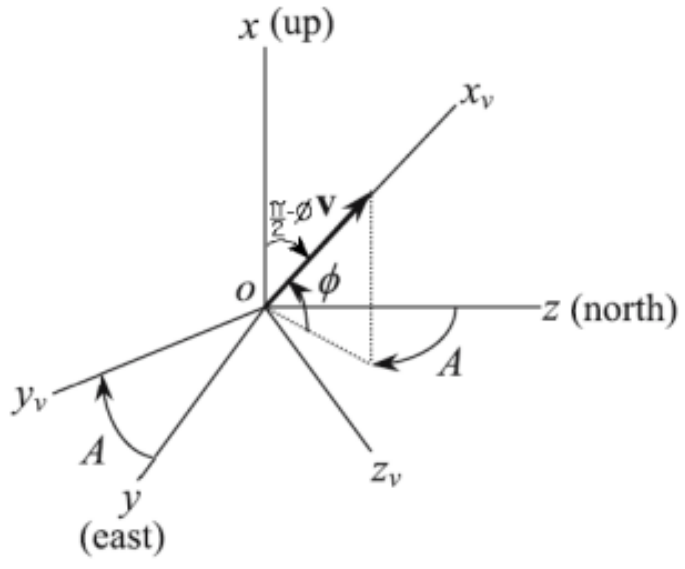
\includegraphics[width=1.5in]{figuras/vento.png}
        \label{fig:refvento}
        \fonte{\cite{livro:andre}}
     \end{center}
\end{figure}

A matriz de transformação do sistema LVLH para o SRV é definida pelo produto de matriz de rotação elementares:

\begin{equation}
C_{srv}^{lvlh} = 
 \left[\begin{array}{lll}
sin \phi & cos\phi sin A & cos\phi cos A \\
0 & cos A & -sinA \\
-cos \phi & sin \phi sin A & sin \phi cosA  
\end{array}\right]
\end{equation}

\subsection{Sistema referencial propulsivo}

O sistema de referência propulsivo é usado para definir o apontamento da força propulsiva com respeito ao SRV. A transformação do SRV para o SRP é encontrada a partir de uma sequência de rotações elementares:

\begin{equation}
C_{srp}^{srv} = 
 \left[\begin{array}{lll}
cos \mu cos \epsilon & sin \mu & -cos \mu sin \epsilon \\
-sin \mu cos \epsilon & cos \mi & sin \mu sin \epsilon \\
sin \epsilon & 0 & cos \epsilon  
\end{array}\right]
\end{equation}

\begin{figure}[h]
    \begin{center}
        \caption{SRP com respeito ao LVLH}
        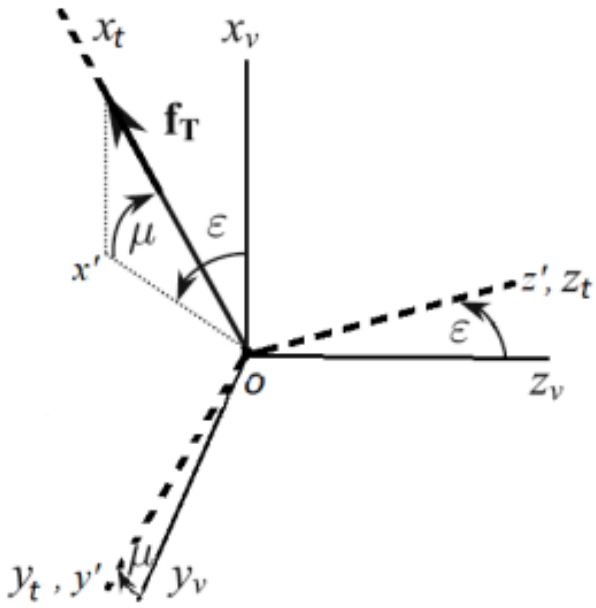
\includegraphics[width=1.5in]{figuras/srp.png}
        \label{fig:SRP}
        \fonte{\cite{livro:andre}}
     \end{center}
\end{figure}

 O SRP é mostrado na figura \ref{fig:SRP}, na qual a origem é o CM do veículo, o eixo $x_{t}$ aponta na direção da força propulsiva, o eixo $z_{t}$ está contido no plano $x_{v}z_{v}$ do SRV, e o eixo $y_{t}$ completa o sistema cartesiano ortogonal da mão direita. 

 \subsection{Força aerodinâmica}

 As forças aerodinâmicas escritas no SRV são dadas por:

 \begin{equation}
     f_{a_{srv}} = \left[\begin{array}{l}
-D \\
f_{y} \\
-L
\end{array}\right]
 \end{equation}

 A força de arrasto D têm sentido oposto à velocidade relativa, enquanto a força de sustentação L é perpendicular à força de arrasto, por fim, a força lateral é perpendicular ao vetor velocidade relativa. 

 \subsection{Força propulsiva}
 A força propulsiva que aponta ao longo do eixo $x_{t}$ com magnitude $f_{T}$ é escrita no SRP como:
\begin{equation}
     f_{T_{srp}} = \left[\begin{array}{l}
f_{T} \\
0 \\
0
\end{array}\right]
 \end{equation}

 No SRV, a força propulsiva é dada por:
\begin{equation}
     f_{T_{srv}} = \left[\begin{array}{l}
f_{T} cos \epsilon cos\mu\\
f_{T} sin\mu\\
-f_{T} cos \mu sin\epsilon
\end{array}\right]
 \end{equation}

Na qual os ângulos  $\mu$ e  $\epsilon$ são a angulação da tubeira em relação à velocidade relativa do veículo, que na prática são os ângulos do guimbal de 2 GDL responsáveis pela fatoração da tração. 

\subsection{Força gravitacional}

A força gravitacional é representada no referencial LVLH como:

\begin{equation}
     f_{g_{lvlh}} = m \left[\begin{array}{l}
-g_{c}\\
0\\
g_{\delta}
\end{array}\right]
 \end{equation}

Assim, a força gravitacional escrita no SRV é dada por:
\begin{equation}
     f_{g_{srv}} = m \left[\begin{array}{l}
-mg_{c}sin\phi + mg_{\delta}cos\phi cos A   \\
-mg\Delta sin A\\
mg_{c}cos\phi + mg_{\delta}sin\phi cos A  
\end{array}\right]
 \end{equation}

 \section{Dinâmica de translação}

 O modelo de mecânica de voo de translação do veículo possui seis equações diferenciais não lineares e três graus de liberdade, para os quais as variáveis de estado são as coordenadas esféricas da posição no referencial PCPF (distância radial $r$, longitude planetária $l$ e latitude $\delta$) e as coordenadas da velocidade relativa escritas no referencial LVLH (magnitude $v$, azimute da velocidade $A$ e elevação $\phi$). As equações são dadas por:


    
\begin{align}
\begin{split}
\dot{v} &= \frac{1}{m} (-D+f_{T}\cos \epsilon \cos\mu + mg_{c} \sin \phi + mg_{\delta} \cos A \cos \phi)\\
&\quad -r\omega_{e}^{2} \cos \delta (\cos A \sin \delta \cos \phi - \cos\delta \sin \phi)
\end{split}\\[1cm]
\begin{split}
\dot{A} &=  \frac{1}{mvcos\phi} (f_{y}+f_{T}\sin \mu - mg_{\delta} \sinA) - \frac{1}{vcos\phi} 2v\omega_{e} (\cosA\cos\delta \sin\phi - \sin\delta \cos\phi)\\
&\quad + \frac{1}{cosv\phi} (r\omega_{e}^{2} \sin A \sin \delta \cos \delta + \frac{v^{2}}{r} \sin A \tan\delta \cos^{2}\phi)
\end{split}\\[1cm]
\begin{split}
\dot{\phi} &= \frac{1}{mv}(L+f_{T} \cos \mu \sin\epsilon - mg_{c} \cos\phi - mg_{\delta}\cos A \sin \phi )\\
&\quad + \frac{1}{v}(2v\omega_{e} \sin A \cos\delta + \frac{v^{2}}{r} \cos \phi + r\omega_{e}^{2} \cos \delta (\cosA\sin\delta \sin\phi + \cos\delta \cos \phi))
\end{split}
\end{align}

%%%%%%%%%%%%% AULA 21 FIM 












































































%% Modelo Atmosferico aula 22

\section{Modelo Atmosférico}

Nesse contexto, vamos explorar os princípios de equilíbrio hidrostático e gás ideal para elaborar perfis verticais correspondentes à pressão, densidade e temperatura sob um estado estacionário de atmosfera padrão. Além disso, iremos estruturar uma variedade de parâmetros adimensionais essenciais para calcular as cargas aerodinâmicas e térmicas.

Ao descrever a atmosfera padrão, estabelecemos uma série de camadas sequenciais, que são caracterizadas pela variação do perfil de temperatura. Na Terra, as camadas são tradicionalmente designadas, em ordem crescente de altitude, como troposfera, estratosfera, mesosfera, termosfera e exosfera.

Algumas constantes termodinâmicas básicas são necessárias para configurar as camadas em equilíbrio termodinâmico. A equação que define a alteração linear da temperatura com a altitude em uma camada específica é:

\begin{equation}
T=T_{i}+a\left(h-h_{i}\right)
\end{equation}

Nessa equação, $i$ representa a camada em questão, $h$ é a altura geométrica e $a$ corresponde à taxa de lapso termal.

A taxa de lapso termal tem uma relação direta com o expoente politrópico $n$, que é crucial para avaliar a estabilidade do equilíbrio hidrostático em uma camada atmosférica. Conforme a seguinte equação, uma camada atmosférica é considerada termicamente estável se $a<0$ e instável se $a>0$.

\begin{equation}
a=-g \frac{1}{R} \frac{n-1}{n}
\end{equation}

Para valores de $a \neq 0$, a pressão como função da altitude geométrica nas camadas com variação linear de temperatura é definida como:

\begin{equation}
p=p_{i}\left(1+\frac{a\left(h-h_{i}\right)}{T_{i}}\right)^{-\frac{g_{0}}{R a}\left(1+\beta\left(\frac{T_{i}}{a}-h_{i}\right)\right)} \exp \left(\frac{g_{0} \beta}{R a}\left(h-h_{i}\right)\right)
\end{equation}

Nessa equação, $g_{0}$ denota a gravidade ao nível do mar, $R$ é a constante específica do gás e $\beta$ é definido por $\beta=2 / r_{0}$, onde $r_{0}$ é o raio médio da Terra.

No caso de camadas isotérmicas $(a=0)$, a pressão como função da altitude geométrica é expressa por:

\begin{equation}
p=p_{i} \exp \left(-\frac{g_{0}}{R T_{i}}\left(h-h_{i}\right)\left(1-\frac{\beta}{2}\left(h+h_{i}\right)\right)\right)
\end{equation}

Depois de calcular a temperatura e a pressão, podemos determinar a densidade utilizando a equação do gás ideal:

\begin{equation}
\rho=\frac{p}{R T}
\end{equation}

As expressões apresentadas são utilizadas para calcular a temperatura, a pressão e a densidade em qualquer altitude até $86 \mathrm{~km}$, faixa na qual a suposição de equilíbrio hidrostático ainda é válida.

Existem múltiplos padrões atmosféricos reconhecidos, com a taxa de variação da temperatura sendo um dos principais parâmetros usados como referência. No curso abordado, optou-se por um modelo misto, conforme proposto por Tewari (2007), que combina dois modelos distintos:

\begin{itemize}
\item No intervalo de $0 \leq h \leq 86 \mathrm{~km}$, aplica-se o padrão da atmosfera dos Estados Unidos de 1976. Este padrão contém duas camadas acima de $86 \mathrm{~km}$, que apresentam variação de temperatura não linear com a altitude e um certo grau de incerteza;

\item Para altitudes superiores a $86 \mathrm{~km}$, é usado o padrão atmosférico americano de 1962. Este padrão representa camadas até a altitude de $h=2000 \mathrm{~km}$, todas com temperatura variável linearmente. A combinação dos padrões atmosféricos dos Estados Unidos de 1976 e 1962 resulta em um modelo de 21 camadas (contando com as subcamadas). Esta combinação é ilustrada na figura abaixo.
\end{itemize}

\begin{figure}[h]
    \begin{center}
        \caption{Combinação de atmosfera padrão norte americana de 1976 e 1962}
        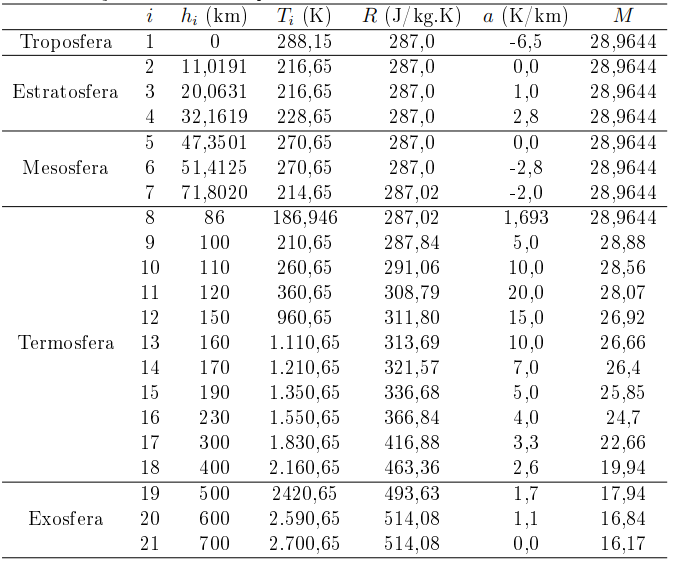
\includegraphics[width=3.5in]{figuras/atmos.png}
        \label{fig:atmos}
        \fonte{(TEWARI,2007), adaptado.}
     \end{center}
\end{figure}

Além das variáveis termodinâmicas básicas, alguns parâmetros adicionais podem ser calculados a partir do modelo atmosférico. Tais parâmetros são úteis para determinar cargas aerotérmicas:

\begin{enumerate}[(a)] 
\item Velocidade do som: 
\begin{equation}
a_{\infty}=\sqrt{\gamma R T}
\end{equation}
\end{enumerate}


\begin{enumerate}[(b)] 
\item Número de Mach:
\begin{equation}
M=\frac{v}{a_{\infty}}
\end{equation}
Onde $v$ representa a velocidade do veículo em relação à atmosfera.
\end{enumerate}

\begin{enumerate}[(c)] 
\item Coeficiente de viscosidade dinâmica:
\begin{equation}
\mu=1,458 \times 10^{-6} \frac{T^{\frac{3}{2}}}{T+110,4}
\end{equation}
\end{enumerate}

\begin{enumerate}[(d)] 
\item Número de Prandtl:
\begin{equation}
\operatorname{Pr}=\frac{\mu c_{p}}{k_{T}}
\end{equation}
Onde $k_{T}$ é o coeficiente de condutividade térmica do gás ideal, enquanto $c_{p}$ é seu calor específico a pressão constante, que pode ser calculado por:
\begin{equation}
c_{p}=\frac{R \gamma}{\gamma-1}
\end{equation}
\end{enumerate}

\begin{enumerate}[(e)] 
\item Número de Knudsen:
\begin{equation}
K n=\frac{\lambda}{l_{c}}
\end{equation}
Onde $\lambda$ é o caminho livre médio do fluxo não perturbado de moléculas e $l_{c}$ é um comprimento característico. O caminho livre médio é baseado no diâmetro de colisão $\sigma$, que pode ser calculado por:
\begin{equation}
\lambda=\frac{m}{\sqrt{2} \pi \sigma^{2} \rho N_{a}}
\end{equation}
Onde $m$ é a massa molecular em $\mathrm{kg} / \mathrm{Mol}$, e $N_{a}=6,0220978 \times 10^{23}$ é o número de Avogadro.
\end{enumerate}

\begin{enumerate}[(f)] 
  \item O parâmetro de regime de escoamento $d$, baseado no número de Knudsen:

  - Se $d=1$, o escoamento é livre molecular. Para $K n \geq 10$;

  - Se $d=2$, o escoamento é contínuo. Para $K n \leq 0,01$;

  - Quando $d=3$, o escoamento é de transição entre os dois regimes. Para $0,01<$ $K n<10$.
\end{enumerate}

\begin{enumerate}[(g)] 
\item Número de Reynolds:
\begin{equation}
R_e =\frac{\rho v l_{c}}{\mu}
\end{equation}
\end{enumerate}


\section{Modelo Gravitacional}

O modelo gravitacional utilizado é o mesmo utilizado no Trabalho 1, as principais hipóteses e pontos que devem ser reforçados são que um campo gravitacional conservativo, aplicado à segunda Lei de Newton para um corpo contínuo, permite a definição do potencial gravitacional:

\begin{equation}
g_i = \frac{\partial \phi_i}{\partial \mathbf{r}_{\mathbf{mi}}} = -Gm_i \frac{\mathbf{r}_{\mathbf{mi}}}{\left\|\mathbf{r}_{\mathbf{mi}}\right\|^3}
\end{equation}


Um modelo gravitacional para um corpo de simetria axial foi utilizado, levando em consideração o potencial gravitacional já descrito no Trabalho 1:

\begin{equation}
\Phi(r, \phi) = \frac{GM}{r}\left(1 - \sum_{n=2}^{\infty}\left(\frac{R_e}{r}\right)^n J_n P_n(\cos \phi)\right)
\end{equation}

Os polinômios de Legendre necessários para o cálculo do potencial são:

\begin{align}
P_2(v) &= \frac{1}{2}\left(3v^2 - 1\right) \\
P_3(v) &= \frac{1}{2}\left(5v^3 - 3v\right) \\
P_4(v) &= \frac{1}{8}\left(35v^4 - 30v^2 + 3\right)
\end{align}

Aplicando o gradiente à função potencial, é possível obter a aceleração da gravidade para coordenadas esféricas:

\begin{equation}
\frac{\partial \Phi}{\partial \mathbf{r}} = \frac{\partial \Phi}{\partial r} \mathbf{i}_r + \frac{\partial \Phi}{\partial \phi} \mathbf{i}_\phi + \frac{1}{r\sin \phi}\frac{\partial \Phi}{\partial \theta} \mathbf{i}_\theta
\end{equation}

\section{Modelo Aerodinâmico}

O modelo aerodinâmico desenvolvido abrange uma ampla faixa de regimes de escoamento, desde subsônico até hipersônico, levando em consideração a densidade do ar desde o meio contínuo até o livre molecular. Além disso, o modelo também incorpora diversos regimes de turbulência, bem como a dependência com a temperatura e reações químicas na termosfera e exosfera.

Em relação aos coeficientes de momento e força, geralmente são calculados três coeficientes de momento: rolagem ($C_{l}$), arfagem ($C_{m}$) e guinada ($C_{n}$); e três coeficientes de força: arrasto ($C_{D}$), sustentação ($C_{L}$) e lateral ($C_{Y}$). No entanto, neste contexto específico, apenas o movimento de translação do foguete é considerado, portanto, os coeficientes de momento não serão modelados. Os coeficientes de força serão avaliados de acordo com as seguintes hipóteses:

\begin{itemize}
    \item Foguetes são otimizados para baixa razão estrutural, o que implica que eles suportam baixos fatores de carga normais ou laterais. Portanto, voam com baixo ângulo de ataque e derrapagem, resultando em forças de sustentação e lateral muito pequenas, as quais podem ser consideradas nulas no modelo.
\end{itemize}

Dentro dessas limitações, apenas o coeficiente de arrasto será tratado. No voo de foguetes, o arrasto é importante para avaliar a perda de velocidade $\Delta v$ que o veículo sofre devido à resistência atmosférica.

Devido à complexidade em estimar modelos de arrasto, será adotado o modelo apresentado na referência (TEWARI, 2007), que é aplicável a uma cápsula de reentrada. No entanto, outros modelos também serão revisados a fim de fazer adaptações no modelo de referência.

Assumiremos que o veículo possui estabilidade estática, o que implica que os ângulos de ataque e derrapagem permaneçam nulos. Nesse caso, o coeficiente de arrasto da cápsula, para uma área de referência da base da cápsula de $S=4 \mathrm{~m}^{2}$, é dado por:

\begin{equation}
\left\{
\begin{array}{lr}
C_{D}=C_{D_{c}} & \text{se } K n<0,0146 \\
C_{D}=C_{D_{f m}} & \text{se } K n>14,5 \\
C_{D}=C_{D_{c}}+\left(C_{D_{f m}}-C_{D_{c}}\right)\left(\frac{1}{3} \log _{10} \frac{K n}{\sin 30^{\circ}}+0,5113\right) & \text{se } 0,0146 \leq K n \leq 14,5
\end{array}
\right.
\end{equation}

onde $K n$ é o número de Knudsen, calculado para o comprimento de referência $l_{c}=0,5 \mathrm{~m}$; $C_{D_{c}}$ é o coeficiente de arrasto no meio contínuo; e $C_{D_{f m}}$ é o coeficiente de arrasto no regime de escoamento livre molecular. O coeficiente $C_{D_{c}}$ é plotado como uma função do número de Mach, conforme ilustrado na Figura \ref{fig:aerodin}.

\begin{figure}[H]
    \begin{center}
        \caption{Coeficiente de arrasto contínuo em função do número de Mach}
        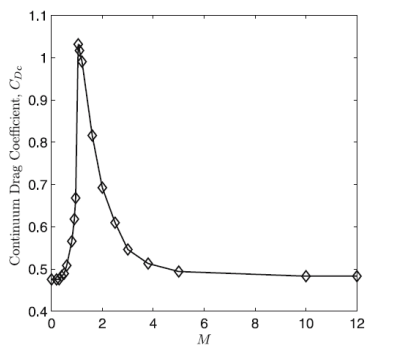
\includegraphics[width=3.5in]{figuras/mach.png}
        \label{fig:aerodin}
        \fonte{(TEWARI,2007).}
     \end{center}
\end{figure}

Podemos ver a partir da Figura \ref{fig:aerodin}, que o princípio de independência do número de Mach hipersônico é válido, tendo em vista que $C_{D_c}$ torna-se invariante com o número de Mach para $M > 8$.




\section{Voo ascendente de foguete}

A partir dos modelos desenvolvidos anteriormente, é possível simular o voo ascendente de um foguete, que possui duas aplicações de interesse: voo de sondagem e voo de inserção orbital.

No voo de sondagem, a trajetória é vertical ou quase vertical, com o objetivo principal de varrer uma faixa de altitude. Geralmente, a missão tem como objetivo adquirir dados em função da altitude ou realizar experimentos em microgravidade. Nesse tipo de trajetória, é necessário que o foguete mantenha uma trajetória vertical de forma estável, geralmente de maneira balística, sem a execução de manobras. Quando o veículo atinge a altitude máxima que atende aos objetivos da missão, a velocidade relativa se aproxima de zero ou se torna muito pequena.

Quanto ao voo de inserção orbital, também é lançado verticalmente ou próximo disso. No entanto, durante a ascensão, a trajetória deve curvar-se gradualmente, de modo que, no momento em que o motor do último estágio é desligado, o ângulo da trajetória seja próximo ou igual a zero. Ao atingir a altitude orbital e desligar o motor do último estágio, a velocidade relativa não será nula. Nesse momento, a velocidade do veículo deve ser igual à velocidade orbital desejada. Portanto, não basta apenas atingir a altitude desejada, mas também é necessário fornecer um impulso de velocidade compatível com a órbita naquela altitude.

A trajetória de inserção orbital pode envolver manobras ou ocorrer de forma puramente balística, dependendo do nível de precisão desejado, das características dos motores, da estabilidade e do controle. Independentemente da presença ou ausência de manobras, a trajetória deve garantir que o ângulo de trajetória seja próximo ou igual a zero no momento da inserção orbital, quando os motores são desligados.

Além das equações de movimento, do modelo aerodinâmico genérico, do modelo atmosférico e do modelo gravitacional mencionados anteriormente, é necessário especificar algumas características básicas do veículo:

\begin{itemize}
    \item Número de estágios;
    \item Massa de propelente de cada estágio;
    \item Massa estrutural de cada estágio;
    \item Massa da carga útil;
    \item Modelo propulsivo de cada estágio: tração e consumo de propelente;
    \item Parâmetros aerodinâmicos de cada estágio.
\end{itemize}

Se o foguete é de múltiplos estágios (N estágios), é necessário inserir na modelagem uma lógica de sequenciamento, a qual deve conter:

\begin{itemize}
    \item Tempo de ignição $t_{i_{k}}$ do estágio $k$, para $k = 1, \ldots, N$. Isso representa o momento em que o k-ésimo estágio é ligado.
   \item Tempo de queima $t_{q_{k}}$ do estágio $k$, para $k = 1, \ldots, N$. Isso representa o momento em que o k-ésimo estágio é desligado.
   \item Tempo de separação $t_{s_{k}}$ do estágio $k$, para $k = 1, \ldots, N$. Isso representa o momento em que o k-ésimo estágio é separado.
\end{itemize}

O sequenciamento de tempos da missão pode ser escrito de maneira relativa:

\begin{itemize}
    \item $t_{i_{k}} = t_{s_{k-1}} + T_{i_{k}}$, para $k = 2, \ldots, N$, onde $T_{i_{k}}$ é o tempo de espera para a ignição do estágio $k$ após a separação do estágio $k-1$.
    \item $t_{q_{k}} = t_{i_{k}} + T_{q_{k}}$, para $k = 1, \ldots, N$, onde $T_{q_{k}}$ é o tempo de duração da queima de propelente do motor do estágio $k$.
    \item $t_{s_{k}} = t_{q_{k}} + T_{s_{k}}$, para $k = 1, \ldots, N$, onde $T_{s_{k}}$ é o tempo de espera para a separação do estágio $k$ após a queima de seu propelente.

\end{itemize}


\subsection{Modelo Propulsivo}

Para o modelo propulsivo é necessário desenvolver os modelos de tração e variação de massa. Para um foguete com $N$ estágios, a variação de massa depende do desacoplamento dos estágios e do consumo de propelente pelos motores. Para os cálculos assumimos uma curva conhecida para a tração em função do tempo. Para determinar a massa em função do tempo, a partir da curva de tração fornecida, podemos utilizar a definição de impulso específico e a fórmula da tração reativa:

\begin{equation}
v_{e_{k}} = g I_{sp_{k}}, \quad f_{T_{k}}(t) = \dot{m}_{p_{k}} v_{e_{k}}
\end{equation}

Assumimos que a variação da tração devido à pressão no bocal de exaustão esteja modelada no impulso específico $I_{sp_{k}}$ ou na velocidade de exaustão $v_{e_{k}}$. Portanto, podemos determinar a relação entre $f_{T_{k}}(t)$ e $\dot{m}_{p_{k}}$ da seguinte forma:

\begin{equation}
\dot{m}_{p_{k}} = \frac{f_{T_{k}}(t)}{g I_{sp_{k}}}
\end{equation}

A vazão mássica de propelente $\dot{m}_{p_{k}}$ e a variação de massa do veículo $\dot{m}$ possuem sinais opostos, pois a vazão de propelente implica na diminuição da massa do veículo. Portanto, para calcular a taxa de variação da massa do veículo, trocamos o sinal de $\dot{m}_{p_{k}}$:

\begin{equation}
\dot{m} = -\frac{f_{T_{k}}(t)}{g I_{sp_{k}}}
\label{eq:252}
\end{equation}

Conhecendo a curva de tração em cada estágio durante a queima de propelente e a lógica de sequenciamento de estágios, o modelo da força propulsiva em função do tempo é dado por:

\begin{equation}
f_{T}(t) = 
\begin{cases}
f_{T_{k}}(t) & , \quad t_{i_{k}} \leq t \leq t_{q_{k}} \\
0 & , \quad t_{q_{k}} < t < t_{i_{k+1}}
\end{cases}
\end{equation}

Como o estágio $k+1$ não inicia sua queima instantaneamente após o estágio $k$, há um intervalo de tempo $\left(t_{q_{k}}, t_{i_{k+1}}\right)$ no qual nenhuma tração é aplicada. Esse intervalo tem duração $T_{s_{k}}+T_{i_{k+1}}$ e é chamado de fase de voo balístico. Em veículos lançadores de propulsão sólida e sem vetorização de tração, as únicas variáveis de controle são os tempos de duração das fases de voo balístico, ou seja, os intervalos de tempo $\left(t_{q_{k}}, t_{i_{k+1}}\right)$.

A lógica para determinação da massa, estágio após estágio, pode ser vista na equação condicional abaixo:

\begin{equation}
m(t) = 
\begin{cases}
m_{0_{1}} = m_{0} & , \quad t_{0} \leq t < t_{i_{1}} \\
m_{0_{k}} - \Delta m_{p_{k}}(t) & , \quad t_{i_{k}} \leq t \leq t_{q_{k}} \\
m_{0_{k}} - m_{p_{k}} & , \quad t_{q_{k}} < t < t_{s_{k}} \\
m_{0_{k+1}} = m_{0_{k}} - m_{p_{k}} - m_{s_{k}} & , \quad t_{s_{k}} \leq t < t_{i_{k+1}}
\label{eq:516}
\end{cases}
\end{equation}



A variável $\Delta m_{p_{k}}(t)$ na Equação \ref{eq:516} é definida como:

\begin{equation}
\Delta m_{p_{k}}(t) = \int_{t_{i_{k}}}^{t} \frac{f_{T_{k}}(\tau)}{g I_{sp_{k}}} d \tau
\end{equation}

No qual assumimos que:

\par - Toda a massa de propelente é consumida durante a queima de cada estágio;
\par - O desacoplamento de cada estágio é instantâneo.

\section{Algoritmos}

Todos os algoritmos desenvolvidos foram feitos de acordo com o fornecido pelo professor e adaptados de acordo com a necessidade do grupo. Os passos gerais do programa são:

\begin{itemize}
    
    \item Dados do veículo lançador e carga paga;

    \item Parâmetros de queima dos estágios;

    \item Parâmetros gerais do lançamento;

    \item Função que cálculo a dinâmica do movimento do veículo lançador;

    \item Funções auxiliares para os cálculos da dinâmica;

    \item Determinação dos parâmetros gerais da órbita;

    \item Plotagem dos gráficos.
    
\end{itemize}

Os programas elaborados para as aulas 19, 26 e 27 foram estruturados com uma função principal em um arquivo, complementada por diversas funções auxiliares dispostas em arquivos separados. No entanto, durante a criação dos códigos para a aula 29, que originalmente seguiam a mesma estrutura, enfrentamos inúmeros problemas relacionados à importação e declaração de variáveis globais, bem como aos inputs de funções.

Isso nos levou a adotar a estratégia de compilar todo o código em um único arquivo. Embora essa alteração tenha aumentado a demanda de processamento para a execução do código, ela permitiu solucionar os erros encontrados e efetivar a transposição do código do Matlab para Python.

É importante enfatizar que essa decisão foi tomada considerando o volume de erros encontrados e o prazo limitado que tínhamos à disposição. Apesar da demanda computacional adicional, consideramos essa medida necessária para cumprir o cronograma estabelecido.
\chapter{Interpretação dos resultados}

Neste capítulo, será abordado a interpretação dos resultados obtidos durante durante a implementação dos códigos e solução dos problemas. Serão analisados os resultados obtidos, relacionando-os com a metodologia e verificando a coerência dos resultados com os fenômenos físicos esperados. 

\section{Cálculo da gravidade de planeta axis simétrico}


O primeiro problema, trata-se da comparação entre os modelos de gravidade para planeta axis simétrico e esférico. As componentes gravitacionais são $g_r$ que está na direção do centro do planeta, porém seu sentido é para fora dele, e $g_{\phi}$ que aponta para o norte no planeta. Os gráficos são representados da forma que $h = 200 km$ quando $\delta = 100 \degree$ e $h = 0 km$ quando $\delta = -100\degree$.

\begin{figure}[H]
\centering
\caption{Comparação entre as componentes da gravidade para um planeta esférico e um axis simétrico.}
\label{fig: Exemplo 3.1}
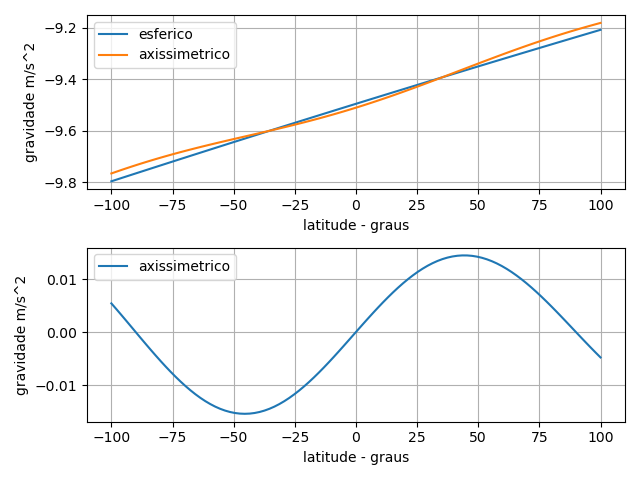
\includegraphics[width=0.8\textwidth]{figuras/Resultados/exemplo31.png}
\fonte{Autores, 2023}
\end{figure}

Observa-se que a componente $g_r$ é igual para ambos os modelos quando a latitude é igual a $\pm 45\degree$ e a componente $g_{\phi}$ é igual no equador e nos polos. A maior diferença entre os modelos pode ser observado para $g_r$ nos polos e para $g_{\phi}$ quando $\delta = \pm 45 \degree$. Ainda, nota-se que a magnitude dessas variações não é tão grande, porém pode gerar um erro gigantesco em simulações de voos de longa duração, praticamente a totalidade das operações aeroespaciais.

\section{Propagação de órbita}

A propagação de órbita permite prever com precisão a posição futura de um objeto em órbita, o que é fundamental para o planejamento de missões espaciais, manobras orbitais, posicionamento de satélites e controle de espaçonaves. Além disso, a propagação de órbita também é utilizada para monitorar o estado de saúde de satélites em órbita, detectar possíveis colisões e realizar ajustes necessários para manter a órbita desejada. Serão apresentadas 3 tipos de órbitas: elíptica; hiperbólica e parabólica, sendo apresentadas as variações da anomalia verdadeira, $\theta$, componente da velocidade na direção x, $v_x$,componente da velocidade na direção y, $v_y$ no tempo, e as coordenadas no plano $XY$.

\subsection{Órbita elíptica}

Uma órbita elíptica é caracterizada por ter a forma de uma elipse. Nesse tipo de órbita, o objeto em movimento descreve uma trajetória oval ao redor do corpo celeste central, como a Terra. A elipse possui dois focos, sendo que o corpo celeste central (como a Terra) está localizado em um dos focos. A figura \ref{fig: Resultado - Propagação de órbita elíptica}, mostra as variações dos parâmetros para esse tipo de órbita. Ainda é considerado o a variação da anomalia excêntrica.

\begin{figure}[H]
\centering
\caption{Propagação de órbita elíptica.}
\label{fig: Resultado - Propagação de órbita elíptica}
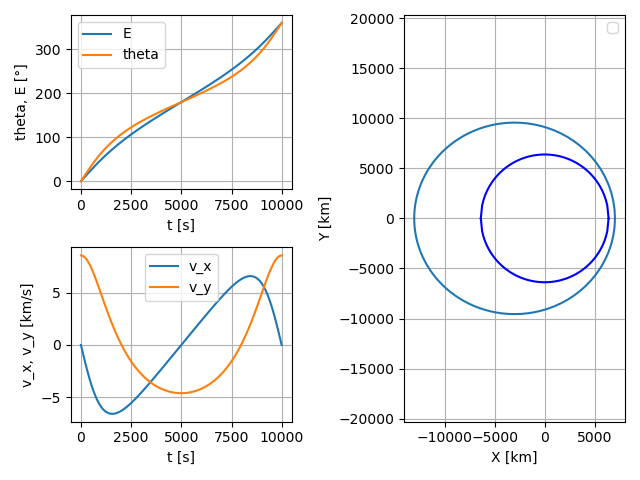
\includegraphics[width=0.8\textwidth]{figuras/Resultados/aula6_eliptica.png}
\fonte{Autores, 2023}
\end{figure}

Como esperado, para a órbita elíptica, a anomalia verdadeira deverá ser igual a anomalia excêntrica nos pontos em que $\theta = n\pi$, para $n$ inteiro, isso ocorre devido ao fato que no periastro e no apoastro as anomalias excêntrica e verdadeira coincidem. Também observa-se que as componentes da velocidade estão coerentes pois $v_x = 0$ quando $v_y = max$, porém o contrário não é válido justamente pelas características da órbita, seria válido apenas para uma órbita circular. Por último o gráfico mais a direita mostra o formato elíptico da órbita.

\subsection{Órbita hiperbólica}

Uma órbita hiperbólica é caracterizada por ter a forma de uma hipérbole. Nesse tipo de órbita, o objeto em movimento descreve uma trajetória aberta, em forma de "U". A velocidade do objeto em relação ao corpo celeste central é suficientemente alta para que ele escape da influência gravitacional e não retorne. Essas órbitas são utilizadas para missões espaciais interplanetárias ou quando se deseja realizar uma trajetória de passagem próxima a um corpo celeste sem entrar em órbita. Para essa órbita também é observado a variação da anomalia hiperbólica.

\begin{figure}[H]
\centering
\caption{Propagação de órbita hiperbólica.}
\label{fig: Resultado - Propagação de órbita hiperbólica}
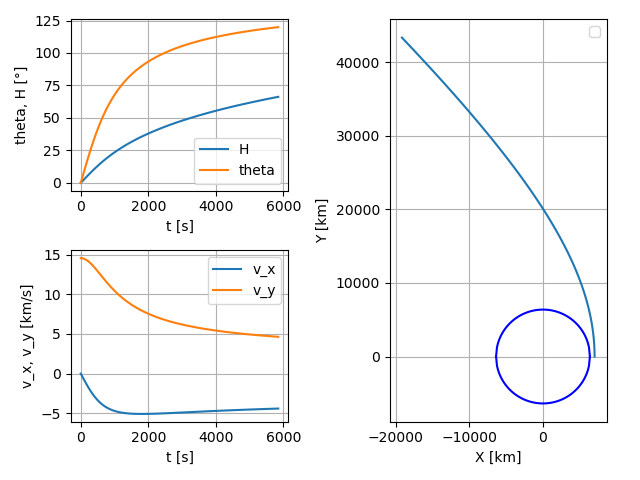
\includegraphics[width=0.8\textwidth]{figuras/Resultados/aula6_hiperbolica.png}
\fonte{Autores, 2023}
\end{figure}

Por se tratar de uma órbita de escape, não existe uma repetição de valores das velocidades como para a órbita elíptica, eles tendem a convergir para algum valor conforme pode ser observado pela figura \ref{fig: Resultado - Propagação de órbita hiperbólica}. Para a anomalia verdadeira, observa-se uma mudança rápida em seu valor e depois um amortecimento fazendo ela tender a um valor, o que também faz sentido por se tratar de uma órbita de escape. Ainda, a anomalia hiperbólica tem sua magnitude menor que a anomalia verdadeira, o que também está coerente já que ela está relacionada a uma função hiperbólica. Por ultimo o gráfico da trajetória representa a forma hiperbólica da trajetória e mostrando a sua posição tendendo para longe da órbita circular.

\subsection{Órbita parabólica}

Uma órbita parabólica é uma órbita especial que está no limite entre as órbitas elípticas e hiperbólicas. Nesse tipo de órbita, o objeto em movimento descreve uma trajetória parabólica. A velocidade do objeto é exatamente suficiente para que ele escape da influência gravitacional do corpo celeste central, mas sem energia cinética adicional para se afastar indefinidamente. Essas órbitas são raras e geralmente ocorrem em situações especiais, como trajetórias de passagem próxima a um corpo celeste ou quando a velocidade de lançamento é cuidadosamente ajustada.

\begin{figure}[H]
\centering
\caption{Propagação de órbita parabólica.}
\label{fig: Resultado - Propagação de órbita parabólica}
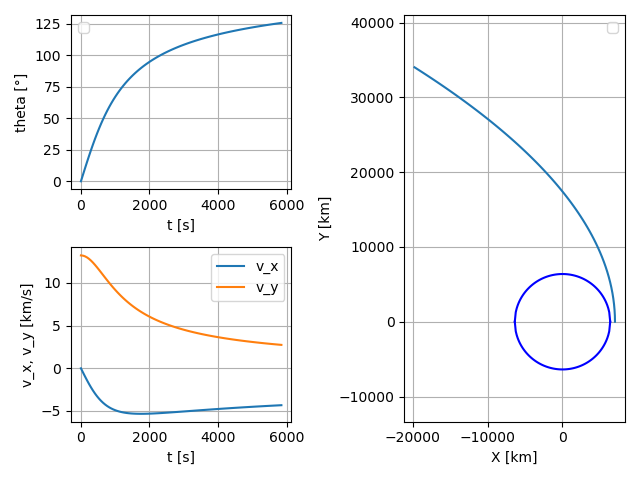
\includegraphics[width=0.8\textwidth]{figuras/Resultados/aula6_parabolica.png}
\fonte{Autores, 2023}
\end{figure}

Da mesma forma que para a órbita hiperbólica, a órbita parabólica é de escape e pode ser observado na figura \ref{fig: Resultado - Propagação de órbita parabólica}. Tanto as componentes da velocidade quanto a anomalia verdadeira são bem parecidas com a órbita hiperbólica o que é bem coerente.

\section{Determinação de órbita}
\par Nessa seção será resolvido um exemplo onde serão obtidos os parâmetros de uma órbita em um problema de dois corpos a partir de uma única observação de posição e velocidade. Os elementos orbitais consistem em 6 parâmetros, que descrevem a progressão e a orientação da órbita. Um conjunto comum de elementos orbitais inclui a excentricidade, semi eixo maior, tempo de periastro, longitude celeste do nodo ascendente, inclinação e argumento de periastro. 
\par Do enunciado tem-se que uma espaçonave observada no referencial centrado na Terra possui a seguinte posição e velocidade celeste: \textbf{r}=-500\textbf{I}+12500\textbf{K} [km] e \textbf{v}=5\textbf{I}-8\textbf{J}[km/s]. Foi solicitado que fosse determinado os parâmetros orbitais. Utilizando o programa desenvolvido em aula, foram obtidos os valores mostrados na tabela \ref{ex52}

\begin{table}[H]
\centering
\caption{Resultados Exemplo 5.2 -Determinação de Órbita}
\begin{tabular}{|c|c|c|}
\hline
Elementos Orbitais & Valor               & Unidade \\ \hline
Semi-Eixo Maior          & -13382.403826218939 & Km      \\ \hline
Excentricidade          & 1.9765961447821856  & - \\ \hline
$\tau$        & 416.7937786907604   & s       \\ \hline
$\Omega$      & 122.0053832080835   & graus   \\ \hline
i          & 71.26309861909091   & graus   \\ \hline
$\omega$      & 95.71519588364482   & graus   \\ \hline
\end{tabular}
\label{ex52}
\end{table}

\par Analisando os elementos pode-se afirmar que a espaçonave se aproxima da Terra, uma vez que $\tau$ é positivo. Isso também pode ser visto devido a anomalia verdadeira no quarto quadrante.

\nocite{book:226549}

\section{Manobras orbitais}

\par As manobras orbitais desempenham um papel crucial na exploração espacial e na operação de satélites, permitindo que espaçonaves e satélites alterem sua posição, velocidade e direção no espaço. Essas manobras são essenciais para alcançar órbitas desejadas, manter a estabilidade orbital, evitar colisões e realizar missões específicas. \par Para uma maior compreensão do assunto e aplicação dos conceitos vistos anteriormente serão discutidos os resultados dos exemplos mostrados a seguir.

\subsection{Exemplo 5.6}

\par É dado que um veículo espacial está em uma órbita terrestre de altitude 500 km, com inclinação de 10\degree , deve ser enviado para uma órbita elíptica com altitudes de perigeu de 200km e apogeu de 700km, bem como inclinação de 5\degree. 
\par Serão aplicados dois impulsos; um para a obtenção da órbita elíptica e o segundo para mudar a inclinação da orbita intermediária, sendo que esse é aplicado no apogeu para minimizar a quantidade de propelente. 
\par O primeiro impulso deve ser aplicado com um ângulo $\beta_1$, uma vez que a altitude de perigeu solicitada é diferente da inicial. Este está relacionado com a velocidade inicial e final.

\par O segundo impulso de velocidade é baseado na variação de inclinação necessária. Da mesma forma, esse deve ser aplicado de formar a minimizar o uso de propelente, isso se dá com a aplicação no apogeu. 

\par Com essas considerações e utilizando o programa desenvolvido em aula, obtém-se os seguintes resultados:

\begin{table}[H]
\centering
\caption{Resultados Exemplo 5.6}
\label{ex56}
\begin{tabular}{|c|c|c|}
\hline
                         & Valor             & Unidade \\ \hline
$\Delta_{v1}$ & 274.066           & m/s     \\ \hline
$\beta_1$                   & 83.12524398118913 & grau    \\ \hline
$\Delta_{v2}$ & 642.5679592057598 & m/s    \\ \hline
$\beta_2$                   & 92.05589473193183 & grau    \\ \hline
\end{tabular}%
\end{table}

\par Comparando as magnitudes dos impulsos, percebe-se que a mudança de inclinação é a manobra que requer um maior incremento de velocidade, utilizando assim a maior quantidade de propelente. Para a otimização de uma dada missão o interessante é lançar a espaçonave o mais próximo possível da inclinação desejada.


\subsection{Exemplo 5.7}

Um veículo espacial em uma órbita terrestre elíptica, com a = 6.900 km, e = 0, 6, $\Omega$ = 120\degree, $\omega$ = 25\degree \ e $i$ = 10\degree. Quando o veículo está no apogeu, um impulso de velocidade é aplicado com um ângulo $\beta$ = 100\degree , relativo ao vetor velocidade, medido no sentido anti-horário em um plano normal à órbita inicial. A magnitude deste impulso é tal que não há alteração da magnitude da velocidade orbital. Determine a nova órbita do veículo espacial.

\par O formato das órbitas será o mesmo, dado que o impulsivo foi aplicado em um plano normal a órbita inicial, não houve alteração da magnitude da velocidade e a distância radial no ponto de manobra não foi alterada, dado as características da manobra. 

\begin{table}[h]
\centering
\caption{Elementos Orbitais da Orbita Resultante - Exemplo 5.7}
\label{tab ex57}
\begin{tabular}{|c|c|c|}
\hline
Elementos Orbitais Finais & Valor               & Unidade \\ \hline
Semi-Eixo Maior                         & 6899999.999         & m       \\ \hline
Excentricidade                        & 0.6000000000000002  & -       \\ \hline
$\Omega$                  & -14.509563087754747 & grau    \\ \hline
$\omega$                     & 158.77278698980075  & grau    \\ \hline
inclinação                       & 11.694220111804377  & grau    \\ \hline
$\alpha$                     & 20.000              & grau    \\ \hline
\end{tabular}%

\end{table}

\par A diferença entre a inclinação inicial e final é de $\delta_i=1.694$. Já o ângulo $\alpha=20\degree$. Como a medida do ângulo $\alpha$ é feita da linha dos nodos na intersecção dos planos orbitais e a medida da inclinação é feita a partir da linha dos nodos da órbita com o plano equatorial, tem-se essa diferença dos ângulos. Com isso conclui-se que uma aplicação de impulso de velocidade não implica em uma alteração da inclinação da nova órbita.
\subsection{Exemplo 5.8}

Foi solicitado o menor impulso total requerido, em uma manobra de transferência orbital bi impulsiva, de uma órbita circular terrestre de 500 km de altitude, para a órbita elíptica vista no exemplo 5.7 que intercepta a circular.
\par Utilizando o script feito em aula, obtém-se os seguintes valores mínimos:

\begin{table}[h]
\centering
\caption{Resultados Exemplo 5.8}
\label{ex58}

\begin{tabular}{|c|c|c|}
\hline
                              & Valor      & Unidade \\ \hline
$v_{at}$                         & 5264.8753  & m/s     \\ \hline
$v_pt$                         & 8450.5766  & m/s     \\ \hline
$v_i$                          & 7612.6039  & m/s     \\ \hline
$v_f$                          & 3800.2669  & m/s     \\ \hline
$\delta_v1 $    & 837.9726   & m/s     \\ \hline
$\delta_v2 $    & -1464.6083 & m/s     \\ \hline
$\delta_{vt}$ & 2302.5810  & m/s     \\ \hline
\end{tabular}

\end{table}

\par Como pode ser visto na tabela acima o menor impulso total requerido é de 2303.581 m/s. 
\subsection{Exemplo 5.9}

Enunciado: Calcule os impulsos de velocidade e o tempo requerido para uma transferência de Hohmann a partir de uma órbita circular terrestre de altitude $250 km$ (órbita de estacionamento - parking orbit), para uma órbita geosíncrona.

\begin{table}[h]
\centering
\caption{}
\label{tab: ex5.9}
\begin{tabular}{|c|c|c|}
\hline
                       & Valor      & Unidade \\ \hline
$\delta_{v1}$                 & $2440.0824$  & $m/s $    \\ \hline
$\delta_{v2}$                 & $1472.0333$  & $m/s$     \\ \hline
Tempo da Transferência & $18961.0618$ & $s$       \\ \hline
\end{tabular}
\end{table}


A transferência de Hohmann é uma manobra orbital amplamente utilizada na engenharia espacial para mover uma espaçonave entre duas órbitas circulares ao redor de um corpo celeste, como a Terra. A manobra é feita com dois impulsos conforme listado abaixo:

\begin{enumerate}

    \item Inserção em órbita de transferência: A espaçonave é colocada em uma órbita elíptica ao redor do corpo celeste de partida. Essa órbita tem um periastro (ponto mais próximo do corpo celeste) na órbita original e um apoastro (ponto mais afastado do corpo celeste) na órbita de destino desejada.

    \item Inserção na órbita de destino: Quando a espaçonave atinge o apoastro da órbita de transferência, uma segunda queima de propulsão é realizada para alterar sua velocidade e direção, de forma a circularizar a órbita na qual deseja-se chegar.

\end{enumerate}

O valor do incremento da velocidade em cada impulso e o tempo para que ocorra a transferência estão dados na tabela \ref{tab: ex5.9}.

\section{Órbitas perturbadas}

\subsection{Exemplo 6.1}

Enunciado: Calcular a inclinação orbital de uma terra sincronizada com o sol
satélite de $a = 6700 km$ e $e = 0.01$.

Ao introduzir uma inclinação em uma órbita sol síncrona, o satélite não permanece fixo em relação ao plano equatorial da Terra. Em vez disso, ele oscila para o norte e para o sul do equador em uma faixa determinada pelo ângulo de inclinação. Isso pode permitir que o satélite tenha uma cobertura mais ampla em termos de latitude, possibilitando a comunicação e observação de áreas que não seriam cobertas por uma órbita geoestacionária padrão. Para as condições dadas calcula-se o valor dos parâmetros $p = 6699.33km$ e $n = 0.0011512156 rad/s$, usando-se $\mu = 3.986004418e^{14}$, $a = 6700e^{3}$, $R_e = 6378.14km$ e $J_2 = 0.00108263$. Assim obtêm-se uma inclinação $i =  96.74779106514552 \degree$. Observa-se uma discrepância de aproximadamente $6.9 \%$ para o valor do livro, o que pode ser justificado pelo valor de $\mu$ escolhido que não é especificado pelo livro e os demais valores estão coerentes.

\subsection{Exemplo 6.2}

Enunciado: Uma espaçonave está em uma viagem interplanetária partindo da Terra. A posição heliocêntrica atual e a velocidade inercial da espaçonave em relação à eclíptica são dadas por

\begin{equation}
R(0) = 
\left[\begin{array}{l}
-27 \\
147.5  \\
0.1
\end{array}\right] \times 10^{6} km, \ 
V(0) = 
\left[\begin{array}{l}
-33 \\
-10  \\
1
\end{array}\right]; km/s
\end{equation}

Os elementos orbitais da Terra calculados a partir de gráficos de efemérides para o tempo presente são os seguintes: $a = 149597870 km$, $e = 0.01667$, $\tau = -100$ \textit{mean solar days}. Determine a posição geocêntrica e a velocidade da espaçonave com $100$  \textit{mean solar days} a partir de agora. 

\begin{figure}[H]
\centering
\caption{Comparação Órbita com Perturbação e Órbita Kepleriana}
\label{fig: 1231}
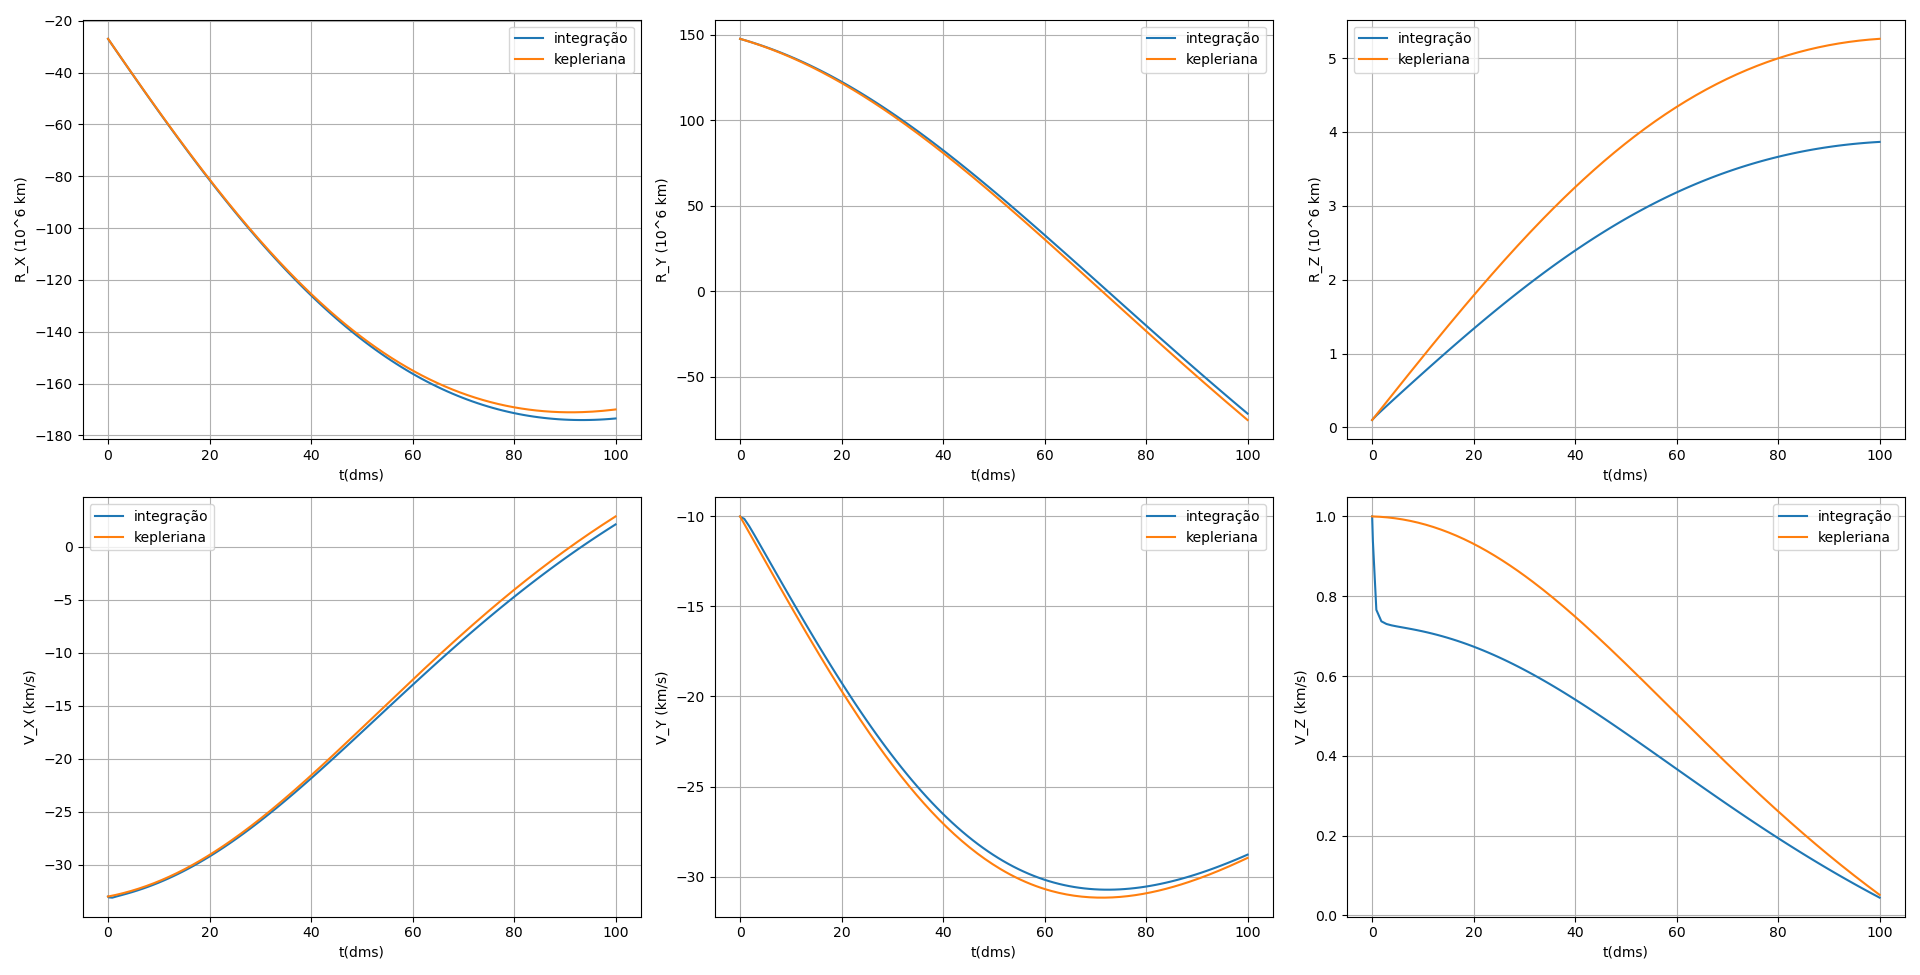
\includegraphics[width=1\textwidth]{figuras/Resultados/ex6.2.png}
\fonte{Autores, 2023}
\end{figure}

A posição inicial da espaçonave está claramente dentro do espaço de influência da terra. No entanto, devido a alta velocidade, a esfera de influência será cruzada nos próximos dias resultando em uma diminuição dessa influência. Conforme a figura \ref{fig: 1231} nota-se que para um espaço de tempo curto a perturbação que é a principal direção de ação da perturbação. conforme maior o tempo considerado maior a diferença entre os modelos evidenciando a impacto das perturbações.

\section{Problema de 3 corpos restrito}
\par Aqui é apresentada a simulação da trajetória de uma espaçonave que passa pelo ponto (0.1,0) no sistema Terra-Lua. Foram simulados os seguintes casos mostrados na tabela abaixo:

\begin{table}[h]
\centering
\caption{Componentes de Velocidade Relativa}
\label{tab:my-table}
\begin{tabular}{|l|l|l|}
\hline
Caso & $\dot{x}$ & $\dot{y}$ \\ \hline
a)    & 0         & 0.5       \\ \hline
b)    & -4        & 1         \\ \hline
c)    & -3.35     & 3         \\ \hline
d)    & -3.37     & 3         \\ \hline
e)    & -3.4      & 3         \\ \hline
f)    & -3.5      & 3         \\ \hline
g)    & -3.6      & 3         \\ \hline
\end{tabular}
\end{table}


Os resultados obtidos podem ser vistos nas figuras a seguir. Destaca-se que os resultados encontrados ficaram ligeiramente diferentes dos obtidos por \cite{book:226549}. Os autores acreditam que a divergência se dá devido ao solver utilizado. No caso deste trabalho foi utilizado o solver \textit{$solve_{ivp}$} com o método "RK45". Já \cite{book:226549} utiliza o solver ODE45 do \textit{Matlab}.


A trajetória para o caso (a) é simulada com um tempo máximo de t = 1  e é ilustrada na figura \ref{fig: cuzao } abaixo. As órbitas em torno da Terra, com rotação apsidal e nodal do plano orbital causada pela gravidade da lua ficam claras na imagem.

\begin{figure}[H]
\centering
\caption{Caso a}
\label{fig: cuzao}
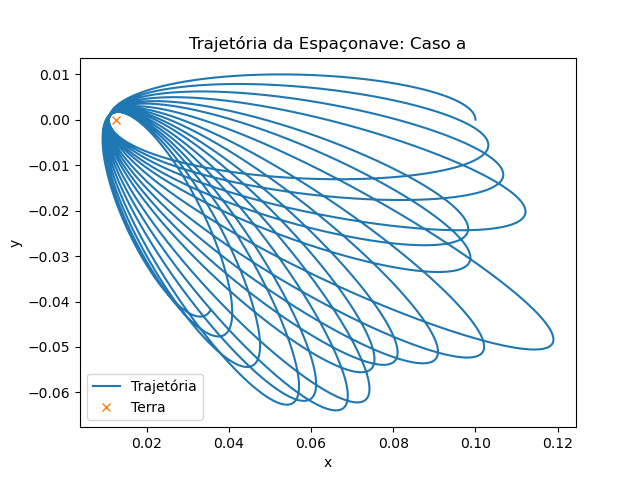
\includegraphics[width=1\textwidth]{figuras/Resultados/7.3/73casoa.png}
\fonte{Autores, 2023}
\end{figure}

\par Com o aumento da velocidade inicial para o caso (b), as órbitas em torno da Terra transformam-se em trajetórias mais energéticas e altamente excêntricas, mesmo assim o veículo  não consegue atravessar o contorno de velocidade zero de C para uma missão lunar. A figura \ref{fig: casobbb} ilustra
o decaimento da órbita com o tempo devido à gravitação da Lua.

\begin{figure}[H]
\centering
\caption{Caso b}
\label{fig: casobbb}
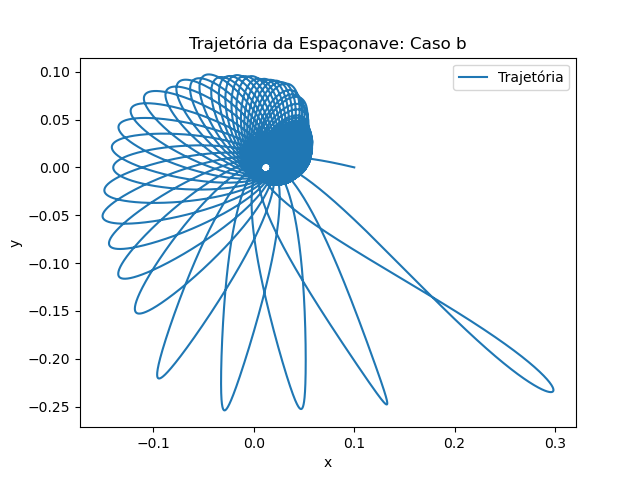
\includegraphics[width=1\textwidth]{figuras/Resultados/7.3/73casob.png}
\fonte{Autores, 2023}
\end{figure}

\par A velocidade inicial do caso (c) é suficientemente grande para uma trajetória de "regresso livre" da Lua para a terra. Neste caso, a nave espacial passa ligeiramente abaixo da órbita da Lua em torno da Terra.

\begin{figure}[H]
\centering
\caption{}
\label{fig: caso c }
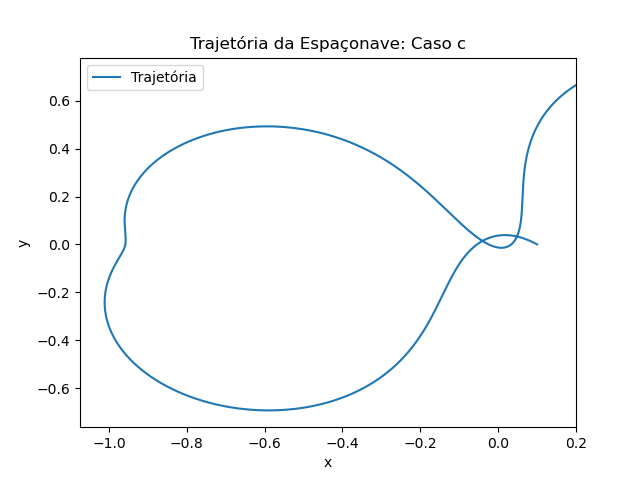
\includegraphics[width=1\textwidth]{figuras/Resultados/7.3/73casoc.png}
\fonte{Autores, 2023}
\end{figure}

\par O tempo total de voo é reduzido significativamente no caso (d) para cerca de t = 2,8, quando a nave espacial passa no entorno da Lua, entre L1 e L2. No processo, a trajetória de regresso tem uma energia cinética ligeiramente maior devido ao impulso dado pelo "estilingue" lunar . As trajetórias lunares de passagem têm sido utilizadas para para impulsionar várias naves espaciais para os pontos lagrangianos sol-terra.

\begin{figure}[H]
\centering
\caption{Caso c}
\label{fig: }
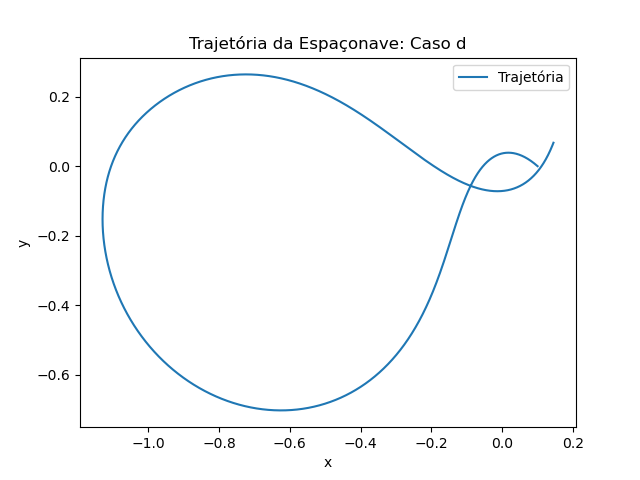
\includegraphics[width=1\textwidth]{figuras/Resultados/7.3/73casod.png}
\fonte{Autores, 2023}
\end{figure}

 No caso (e) , o tempo de voo cresce para cerca de
 t = 3.45 para uma volta completa, uma vez que a espaçonave passa mais longe da lua, passando depois do ponto L1.


\begin{figure}[H]
\centering
\caption{Caso d}
\label{fig: }
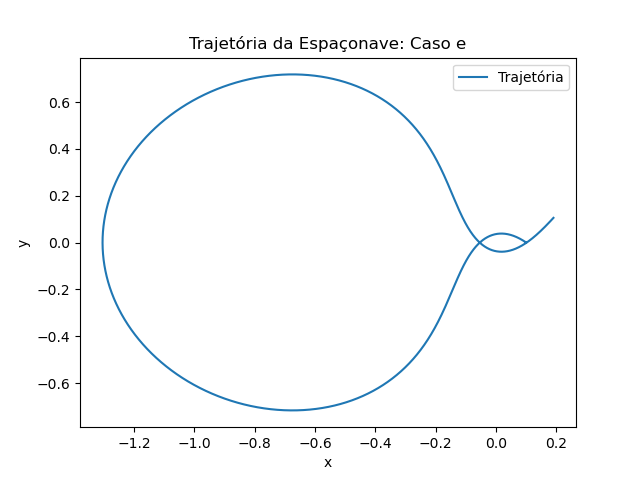
\includegraphics[width=1\textwidth]{figuras/Resultados/7.3/73casoe.png}
\fonte{Autores, 2023}
\end{figure}

Para os casos $f$ e $g$, figuras \ref{fig: f} e \ref{fig: g} respectivamente, há diferenças qualitativas nas trajetórias. é observado que para um longo tempo o caso $f$ demonstra que a espaçonave faz uma passagem pela lua a uma grande distância de $L_1$, porém é incapaz de escapar da gravidade terrestre, fazendo se aproximar mais da lua na próxima passagem, conforme mais passagens ocorrem a espaçonave é trazida para a órbita da terra com um decrescimento do raio. O caso $f$ ilustra um método mais barato para trazer um satélite para uma órbita geossíncrona, através de múltiplas passagens através da lua. Um método similar é encontrado para múltiplas passagens em planetas para diminuir o custo de missões interplanetárias.

Conforme ocorre o aumento da energia inicial para o caso $g$, a espaçonave não retorna para terra e sim embarca em uma trajetória de escape do sistema terra-lua. Nessa trajetória, a vantagem encontra-se na ajuda recebida pela gravidade lunar reduzindo o consumo de combustível e consequentemente o custo de missões interplanetárias.

\begin{figure}[H]
\centering
\caption{Caso f}
\label{fig: f}
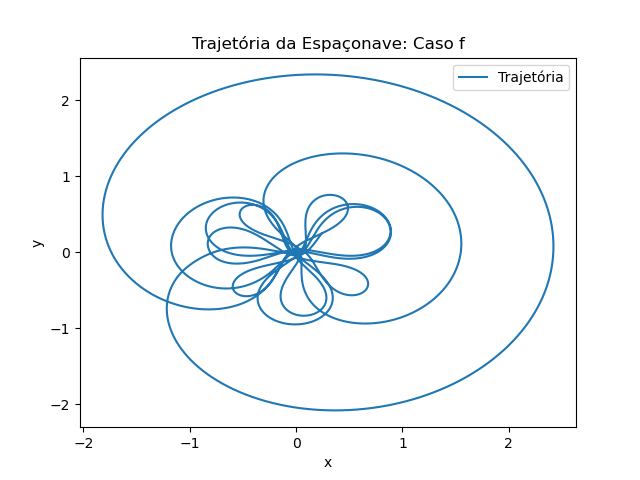
\includegraphics[width=1\textwidth]{figuras/Resultados/7.3/73casof.png}
\fonte{Autores, 2023}
\end{figure}

\begin{figure}[H]
\centering
\caption{Caso g}
\label{fig: g}
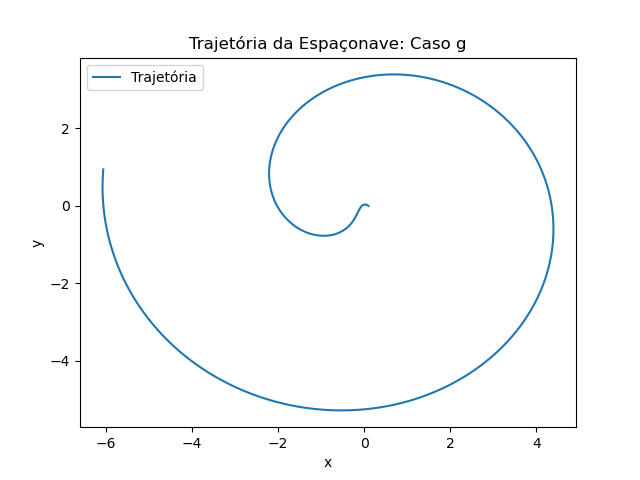
\includegraphics[width=1\textwidth]{figuras/Resultados/7.3/73casog.png}
\fonte{Autores, 2023}
\end{figure}
\input{Texto/Conclusão}
	
	
% % % % % % % % % % % % % % % % % % % % % % % % % % % % % % % % % % % % % % 
% % % % % % % % % % % % FIM DAS PAGINAS TEXTUAIS % % % % % % % % % % % % % % 
% % % % % % % % % % % % % % % % % % % % % % % % % % % % % % % % % % % % % % 



% % % % % % % % % % % % % % % % % % % % % % % % % % % % % % % % % % % % % % 	
% % % % % % % % % % % % % BIBLIOGRAFIA  % % % % % % % % % % % % % % % % % % 
% % % % % % % % % % % % % % % % % % % % % % % % % % % % % % % % % % % % % % 	

\startbibliography % comando para formatar na MDT UFSM
\bibliography{referencias}

	
% % % % % % % % % % % % % % % % % % % % % % % % % % % % % % % % % % % % % 	
% % % % % % % % % % % % % APENDICES % % % % % % % % % % % % % % % % % % %
% % % % % % % % % % % % % % % % % % % % % % % % % % % % % % % % % % % % % 	
\apendice %%%% TEXTOS A PARIR DESTE PONTO SERAO CONSIDERADOS APENDICES

\end{document}
